%%%%%%%%%%%%%%%%%%%%%%%%%%%%%%%%%%%%%%%%%
% Masters/Doctoral Thesis 
% LaTeX Template
% Version 1.43 (17/5/14)
%
% This template has been downloaded from:
% http://www.LaTeXTemplates.com
%
% Original authors:
% Steven Gunn 
% http://users.ecs.soton.ac.uk/srg/softwaretools/document/templates/
% and
% Sunil Patel
% http://www.sunilpatel.co.uk/thesis-template/
%
% License:
% CC BY-NC-SA 3.0 (http://creativecommons.org/licenses/by-nc-sa/3.0/)
%
% Note:
% Make sure to edit document variables in the Thesis.cls file
%
%%%%%%%%%%%%%%%%%%%%%%%%%%%%%%%%%%%%%%%%%


\newcommand{\bibnamefont}{}
\newcommand{\citenamefont}{}
\newcommand{\bibfnamefont}{}
\newcommand{\urlprefix}{}
\newcommand{\url}{}

%----------------------------------------------------------------------------------------
%	PACKAGES AND OTHER DOCUMENT CONFIGURATIONS
%----------------------------------------------------------------------------------------

\documentclass[11pt, oneside]{Thesis} % The default font size and one-sided printing (no margin offsets)

\graphicspath{{Pictures/}} % Specifies the directory where pictures are stored

\usepackage[square, numbers, comma, sort&compress]{natbib} % Use the natbib reference package - read up on this to edit the reference style; if you want text (e.g. Smith et al., 2012) for the in-text references (instead of numbers), remove 'numbers' 
\hypersetup{urlcolor=blue, colorlinks=true} % Colors hyperlinks in blue - change to black if annoying
\title{\ttitle} % Defines the thesis title - don't touch this

\usepackage{simplewick}
\usepackage{placeins}
\usepackage[para,online,flushleft]{threeparttable}

\begin{document}
%\maketitle2
\frontmatter % Use roman page numbering style (i, ii, iii, iv...) for the pre-content pages

\setstretch{1.3} % Line spacing of 1.3

% Define the page headers using the FancyHdr package and set up for one-sided printing
\fancyhead{} % Clears all page headers and footers
\rhead{\thepage} % Sets the right side header to show the page number
\lhead{} % Clears the left side page header

\pagestyle{fancy} % Finally, use the "fancy" page style to implement the FancyHdr headers

\newcommand{\HRule}{\rule{\linewidth}{0.5mm}} % New command to make the lines in the title page

% PDF meta-data
\hypersetup{pdftitle={\ttitle}}
\hypersetup{pdfsubject=\subjectname}
\hypersetup{pdfauthor=\authornames}
\hypersetup{pdfkeywords=\keywordnames}

%----------------------------------------------------------------------------------------
%	TITLE PAGE
%----------------------------------------------------------------------------------------

\begin{titlepage}
\begin{center}

\textsc{\LARGE University of Oslo}\\[1.5cm] % University name
\textsc{\Large Master Thesis}\\[0.5cm] % Thesis type
  \vspace{10mm}          % Vertikalt mellomrom
%\HRule \\[0.4cm] % Horizontal line
{\huge \bfseries \ttitle}\\[0.4cm] % Thesis title
%\HRule \\[1.5cm] % Horizontal line
 
%\begin{minipage}{0.4\textwidth}
%\begin{flushleft} \large
%\emph{Author:}\\
%\href{http://www.johnsmith.com}{\authornames} % Author name - remove the \href bracket to remove the link
%\end{flushleft}
%\end{minipage}
%\begin{minipage}{0.4\textwidth}
%\begin{flushright} \large
%\emph{Supervisor:} \\
%\href{http://www.jamessmith.com}{\supname} % Supervisor name - remove the \href bracket to remove the link  
%\end{flushright}
%\end{minipage}\\[3cm]
 \vspace{15mm}
 \centerline{
\includegraphics[width=5cm,height=5cm]{figures/apollonseglet/Apollonseglet/UiO_Segl_cmyk.pdf}}
%
\includegraphics{figures/apollonseglet/Apollonseglet/UiO_Segl_cmyk.pdf}
\vspace{15mm}
\large \textit{A thesis submitted in fulfilment of the requirements\\ for the degree of \degreename}\\[0.3cm] 
% University requirement text
\textit{in the}\\[0.4cm]
\groupname\\\deptname\\[2cm] % Research group name and department name
 
{\large \today}\\[4cm] % Date
%\includegraphics{Logo} % University/department logo - uncomment to place it

 
\vfill
\end{center}

\end{titlepage}

%----------------------------------------------------------------------------------------
%	DECLARATION PAGE
%	Your institution may give you a different text to place here
%----------------------------------------------------------------------------------------

%\Declaration{

%\addtocontents{toc}{\vspace{1em}} % Add a gap in the Contents, for aesthetics

%I, \authornames, declare that this thesis titled, '\ttitle' and the work presented in it are my own. I confirm that:

%\begin{itemize} 
%\item[\tiny{$\blacksquare$}] This work was done wholly or mainly while in candidature for a research degree at this University.
%\item[\tiny{$\blacksquare$}] Where any part of this thesis has previously been submitted for a degree or any other qualification at this University or any other institution, this has been clearly stated.
%\item[\tiny{$\blacksquare$}] Where I have consulted the published work of others, this is always clearly attributed.
%\item[\tiny{$\blacksquare$}] Where I have quoted from the work of others, the source is always given. With the exception of such quotations, this thesis is entirely my own work.
%\item[\tiny{$\blacksquare$}] I have acknowledged all main sources of help.
%\item[\tiny{$\blacksquare$}] Where the thesis is based on work done by myself jointly with others, I have made clear exactly what was done by others and what I have contributed myself.\\
%\end{itemize}
 
%Signed:\\
%\rule[1em]{25em}{0.5pt} % This prints a line for the signature
 
%Date:\\
%\rule[1em]{25em}{0.5pt} % This prints a line to write the date
%}

\clearpage % Start a new page

%----------------------------------------------------------------------------------------
%	QUOTATION PAGE
%----------------------------------------------------------------------------------------

\pagestyle{empty} % No headers or footers for the following pages

\null\vfill % Add some space to move the quote down the page a bit

\textit{``What I cannot create, I do not understand."}

\begin{flushright}
Richard Feynman
\end{flushright}

\vfill\vfill\vfill\vfill\vfill\vfill\null % Add some space at the bottom to position the quote just right

\clearpage % Start a new page

%----------------------------------------------------------------------------------------
%	ABSTRACT PAGE
%----------------------------------------------------------------------------------------

\addtotoc{Abstract} % Add the "Abstract" page entry to the Contents

\abstract{\addtocontents{toc}{\vspace{1em}} % Add a gap in the Contents, for aesthetics

We investigate how the coupled cluster triples amplitudes contributes to the ground state energy for the homogeneous electron gas. Beginning with first principles, we incrementally derive the formalism and equations needed, and describe in detail how two independent and conceptually differing computational schemes may be implemented efficiently for the system. We finally perform numerous calculations for the system, investigate how the gradual inclusion of more diagrams leading up to the full coupled cluster doubles triples (CCDT) method affects the energy, and we estimate the energy in the thermodynamical limit by extrapolating results from large scale computations on the Abel cluster.
}

\clearpage % Start a new page

%----------------------------------------------------------------------------------------
%	ACKNOWLEDGEMENTS
%----------------------------------------------------------------------------------------

\setstretch{1.3} % Reset the line-spacing to 1.3 for body text (if it has changed)

\acknowledgements{\addtocontents{toc}{\vspace{1em}} % Add a gap in the Contents, for aesthetics

%The acknowledgements and the people to thank go here, don't forget to include your project advisor\ldots

The content of this thesis relies heavily on the work of others. While the many physicist who paved way for this work is far too many to each be mentioned by name, I would like to extend my appreciation of them all. Without their valuable contributions, we may still have been standing paralyzed when faced with the discrete nature of the universe. After years as a student of physics, I'm more impressed and perplexed than ever by the fact that someone could come up with the concepts of wave functions to describe these phenomenas.

Of the more direct contributions to this thesis, I wish to acknowledge the many made by my advisor, prof. Morten Hjorth-Jensen. His valuable and deep insight into many-body theory as well as the broader context of physics has been extremely helpful. His liberal approach to guidance has allowed me to also explore some of my own ideas and paths - even some detours - which I suspect may have resulted in some more confidence from my part when dealing with such matters as science. The time spent under his supervision at Michigan State University was very rewarding and productive.

Another direct contributor to this thesis is Gustav Baardsen, ph.d. In large parts, this thesis is founded on his doctoral thesis \emph{Coupled-cluster theory for infinite matter} \cite{Baardsen2014}. He has also been very helpful in supplying me with his code, as well as very extensive datasets for comparison with my own.

It has also been of great help to be part of the Computational Physics group at the University of Oslo. Everything from minor discussions on which libraries to utilize or how to install drivers for the printer, to more central issues as how to compile armadillo on the Abel cluster (Thank you Jørgen Høgberget and Svenn-Arne Dragly) have been extremely valuable in my work. I am proud to be a member of this highly competent group.

Finally I wish to thank my family: my dear Kine for her care, understanding and dedication, as well as our two sons Erik and Alfred for allowing me to sleep after late nights working on this project.

As mentioned, some of the calculations in this thesis was performed on the Abel Cluster, owned by the University of Oslo and the Norwegian metacenter for High Performance Computing (NOTUR), and operated by the Department for Research Computing at USIT, the University of Oslo IT-department. \cite{abel} I am grateful for being trusted with access to these overwhelming resources.
}
\clearpage % Start a new page

%----------------------------------------------------------------------------------------
%	LIST OF CONTENTS/FIGURES/TABLES PAGES
%----------------------------------------------------------------------------------------

\pagestyle{fancy} % The page style headers have been "empty" all this time, now use the "fancy" headers as defined before to bring them back

\lhead{\emph{Contents}} % Set the left side page header to "Contents"
\tableofcontents % Write out the Table of Contents

\lhead{\emph{List of Figures}} % Set the left side page header to "List of Figures"
\listoffigures % Write out the List of Figures

\lhead{\emph{List of Tables}} % Set the left side page header to "List of Tables"
\listoftables % Write out the List of Tables

%----------------------------------------------------------------------------------------
%	ABBREVIATIONS
%----------------------------------------------------------------------------------------

%\clearpage % Start a new page

%\setstretch{1.5} % Set the line spacing to 1.5, this makes the following tables easier to read

%\lhead{\emph{Abbreviations}} % Set the left side page header to "Abbreviations"
%\listofsymbols{ll} % Include a list of Abbreviations (a table of two columns)
%{
%\textbf{LAH} & \textbf{L}ist \textbf{A}bbreviations \textbf{H}ere \\
%\textbf{SD} & \textbf{S}slater \textbf{D}eterminant \\
%\textbf{CCM} & \textbf{C}coupled \textbf{C}luster \textbf{M}ethod \\
%\textbf{SP} & \textbf{S}ingle \textbf{P}article \\
%\textbf{Acronym} & \textbf{W}hat (it) \textbf{S}tands \textbf{F}or \\
%\textbf{Acronym} & \textbf{W}hat (it) \textbf{S}tands \textbf{F}or \\
%\textbf{Acronym} & \textbf{W}hat (it) \textbf{S}tands \textbf{F}or \\

%\textbf{Acronym} & \textbf{W}hat (it) \textbf{S}tands \textbf{F}or \\
%}

%----------------------------------------------------------------------------------------
%	PHYSICAL CONSTANTS/OTHER DEFINITIONS
%----------------------------------------------------------------------------------------

%\clearpage % Start a new page

%\lhead{\emph{Physical Constants}} % Set the left side page header to "Physical Constants"

%\listofconstants{lrcl} % Include a list of Physical Constants (a four column table)
%{
%Speed of Light & $c$ & $=$ & $2.997\ 924\ 58\times10^{8}\ \mbox{ms}^{-\mbox{s}}$ (exact)\\
% Constant Name & Symbol & = & Constant Value (with units) \\
%}

%----------------------------------------------------------------------------------------
%	SYMBOLS
%----------------------------------------------------------------------------------------

%\clearpage % Start a new page

%\lhead{\emph{Symbols}} % Set the left side page header to "Symbols"

%\listofnomenclature{lll} % Include a list of Symbols (a three column table)
%{
%$a$ & distance & m \\
%$P$ & power & W (Js$^{-1}$) \\
% Symbol & Name & Unit \\

%& & \\ % Gap to separate the Roman symbols from the Greek

%$\omega$ & angular frequency & rads$^{-1}$ \\
%% Symbol & Name & Unit \\
%}

%----------------------------------------------------------------------------------------
%	DEDICATION
%----------------------------------------------------------------------------------------

%\setstretch{1.3} % Return the line spacing back to 1.3

%\pagestyle{empty} % Page style needs to be empty for this page

%\dedicatory{For/Dedicated to/To my\ldots} % Dedication text

%\addtocontents{toc}{\vspace{2em}} % Add a gap in the Contents, for aesthetics

%--------
%  Defining some "macros" (don't know what they are called
%------

\newcommand{\Cr}[1]{\hat{a}_{#1}^\dagger}
\newcommand{\An}[1]{\hat{a}_{#1}}

\newcommand{\Up}[1]{{#1}_\uparrow}
\newcommand{\Dn}[1]{{#1}_\downarrow}




%----------------------------------------------------------------------------------------
%	THESIS CONTENT - CHAPTERS
%----------------------------------------------------------------------------------------

\mainmatter % Begin numeric (1,2,3...) page numbering

\pagestyle{fancy} % Return the page headers back to the "fancy" style

% Include the chapters of the thesis as separate files from the Chapters folder
% Uncomment the lines as you write the chapters
% Chapter Template

\stepcounter{section}

\chapter{Introduction} % Main chapter title

\label{Preface} % Change X to a consecutive number; for referencing this chapter elsewhere, use \ref{ChapterX}

\lhead{\emph{Introduction}} % Change X to a consecutive number; this is for the header on each page - perhaps a shortened title

%----------------------------------------------------------------------------------------
%	Theory
%----------------------------------------------------------------------------------------

In this thesis we will use the coupled cluster method, also called coupled cluster \emph{theory}, to investigate the homogeneous electron gas. More specifically, we will investigate how inclusion of triple excitations in the coupled cluster equations will affect calculations of the ground state energy.  Numerous (see for example Refs.~\cite{Baardsen2014, Shepherd2012, Roggero2013}) calculations of the system in question has been made using the coupled cluster doubles (CCD) method, doubles with perturbative triples (CCD(T)), and various other many-body methods, but to the author's best knowledge this thesis presents for the first time results containing triple excitations for the electron gas.

We shall systematically investigate how each diagram present in the equation contributes to the ground state energy for smaller basis sets, incrementally leading up the the full inclusion of triple excitations (CCDT), and we will estimate the energy in the thermodynamical limit using a CCDT-1 \cite{ShavittBartlett2009} approach and compare these results with existing results from full configuration interaction quantum monte carlo (FCIQMC) present in the literature.

In the second chapter of this thesis \ref{Chapter1}, we review the context from which the many-body problem arise, and we motivate the need for the formalism developed in Chapters \ref{Chapter2} and \ref{Chapter3}. In Chapter \ref{Chapter4}, we give a broad overview of the methodology involved, and we give some special attention to the methods that closely relates to the coupled cluster method, such as Hartree-Fock theory, configuration interaction theory and many-body perturbation theory.

In Chapter \ref{Chapter5}, we derive the coupled cluster method, and we introduce both diagrammatic techniques and computational implementations of these that we use to derive the actual equations for various truncations of the coupled cluster method.

The homogeneous electron gas (HEG) is reviewed in Chapter \ref{Chapter6}, where we derive and present expressions needed to evaluate the coupled cluster equations, such as the the plane wave basis, Fock matrix elements \cite{Thijssen}, the two-body interaction \cite{ShavittBartlett2009} and the general structure of the model. We also place this thesis into context with newly published material on the system.

In Chapter \ref{Chapter7} we present implementational details, and we describe two conceptually different schemes for solving the coupled cluster equations for our system. We also discuss topics such as performance and memory usage.

In the final Chapter \ref{Chapter8}, we validate the implementations by comparing with results published in other studies and by comparing results from the two independent solvers. We then perform a series of calculations for smaller basis sets, ending up with the full inclusion of triple amplitudes. Estimates in the thermodynamical limit is performed by extrapolation from a data set obtained by running our CCDT-1 code on the Abel cluster (see Ref.~\cite{abel}).

We discuss these findings in light of calculations performed by others, and we finally give some concluding remarks, recommendations and future prospects.













% Chapter Template

\stepcounter{section}

\chapter{Many Body Quantum Theory} % Main chapter title

\label{Chapter1} % Change X to a consecutive number; for referencing this chapter elsewhere, use \ref{ChapterX}

\lhead{Chapter 2. \emph{Many Body Quantum Theory}} % Change X to a consecutive number; this is for the header on each page - perhaps a shortened title

%----------------------------------------------------------------------------------------
%	Theory
%----------------------------------------------------------------------------------------

\paragraph{A brief review} The aim of this chapter is to introduce some of the  fundamental concepts relevant to this thesis, with an emphasis on many-body theory and the formalism of second quantization.


\section{Many-body Theory}

Many-body theory is the framework which to date best describes and
predicts phenomena relating to interacting quantum systems. The main
body of the theory was developed by physicists such as Fermi, Pauli
and Dirac in the late 1920s. As the Davisson-Germer electron
diffraction experiment confirmed the particle wave duality of matter
in 1927 \cite{Giuliani2005} and the discovery of half integer spin was
made by Goudsmit and Uhlenbeck in 1925 \cite{Giuliani2005}, these
results found their rationale in the theoretical work of Pauli, Fermi
and Dirac \cite{Giuliani2005}. Dirac introduced the 
\emph{Second Quantization Formalism} in 1927 \cite{ShavittBartlett2009}.

Important contributions have been made continuously over the
years. Feynman introduced the diagrammatic formalism in
1949 \cite{ShavittBartlett2009}, prior to the advent of many-body
perturbation theory, introduced by Brueckner and Levinson in
1955 \cite{ShavittBartlett2009}.  The subsequent decades have seen an
explosion in the development of various so-called first principle
methods\footnote{With first principle or {\em ab initio} methods, we
mean methods that allow, with a given Hamiltonian, for either exact
solutions of the many-body problem or approximative solutions which
can be improved upon systematically}, including several Monte Carlo
methods, Green's function methods, full configuration interaction
theory and many other many-body approaches. In this thesis, we will in particular pay
attention to coupled cluster theory. This method was originally
introduced in order to solve the nuclear many-body problem by Coester
and Kümmel \cite{Kummel}.  Coupled cluster theory, with its various
approximations, has during the last five decades provided highly
accurate predictions for a wide range of interacting quantum systems
and has become one of the standard many-body methods in quantum
chemistry and nuclear physics, providing precise benchmarks for
systems up to hundreds of interacting electrons or nucleons.

Coupled cluster theory offers a range of methods for approximating energies and
properties of systems. When choosing which method to utilize, one has
to consider the trade off between performance and accuracy. While some
approximations  may in principle provide us with very precise results, they may
have computational requirements beyond what is currently
achievable. With these considerations, the so-called 
CCSD(T) (Coupled Cluster Singles and Doubles with Perturbative
Triples) is considered to be the "gold standard" of coupled cluster theory, as it is
both efficient and highly accurate.\footnote{The author was not able
to pinpoint exactly where this concept of "gold-standard" originated,
but a search on Google Scholar with the keywords "coupled cluster gold
standard" clearly shows that this terminology is commonly used within
the quantum chemistry community.}

In the following sections we will briefly review some of the essential elements of quantum many-body theory and
introduce notations used in the rest of this thesis. Since a great  number of in-depth and
excellent modern textbooks are written on these topics, the aim here 
is merely to introduce concepts and theory that will be utilized in
later parts of this thesis. For an extensive introduction to the basic elements of many-body theory, 
the reader is referred to some of the many books on the
subject. \cite{ShavittBartlett2009, Szabo, Harris, GrossRungeHeinonen,Thijssen}.


%-----------------------------------
%	The Fundamental postulates of Quantum Mechanics
%-----------------------------------
\section{The Postulates of Quantum Mechanics}

The mathematical framework of quantum mechanics is rooted in several
fundamental postulates. We will here briefly state these.

\paragraph{(1) The Wave Function}
The state of a quantum mechanical system is fully specified in time and space by a wave function $\vert \Psi(x,t) \rangle$. Born's Statistical Interpretation \cite{Griffiths2005} suggests that the probability of finding the system in the volume element $dx$ at time $t$ is defined by $\Psi(x,t)^* \Psi(x,t) dx$. Another important property is that the wave function should be normalized to one in the full occupied space $\Omega$ \cite{Griffiths2005}, that is

$$ \int_\Omega \Psi(\mathbf{x},t)^* \Psi(\mathbf{x},t) d\Omega = 1. $$

Here the variable $\mathbf{x}$ can represent one or more-dimensional systems and include for example spin degrees of freedom. 
\paragraph{(2) Observables} For any measurable quantity, such as energy, momentum, or spin, there exists a corresponding linear, Hermitean operator. Such operators are commonly denoted with a hat; $\hat{A}$

\paragraph{(3) Measurement} A measurement of any observables linked with the operator $\hat{A}$ acting on a given system, will result in a value $a$, corresponding to the eigenvalues of the equation

$$ \hat{A} \vert \Psi \rangle = a \vert \Psi \rangle. $$

\paragraph{(4) Average measurement} For a system in the state $\vert \Psi \rangle$, we define the average measurement of $\hat{A}$ by

 $$ \int_{\Omega} \Psi(\mathbf{x},t)^* \hat{A} \Psi(\mathbf{x},t) d\Omega \equiv \langle  \Psi \vert  \hat{A} \vert \Psi \rangle  =  \langle{ A} \rangle.$$
Here we have assumed that the wave function is normalized.
The average measurement is \emph{not the most likely result}, merely the average of a multitude of measurements on identical systems. 

\paragraph{(5) Time evolution} The system will evolve in time in accordance with the time independent Schrödinger equation

\begin{equation}
\hat{H} \vert \Psi(x,t) \rangle = i\hbar \frac{\partial}{\partial t} \vert \Psi(x,t) \rangle .
\label{eqn:tisl}
\end{equation}

While the more general requirement of a wave function is that it fulfills the time dependent Schrödinger equation, we may also seek stationary solutions to the \emph{time independent} Schrödinger equation

\begin{equation}
\hat{H} \vert \Psi(x) \rangle = \epsilon \vert \Psi(x) \rangle,
\label{eqn:tusl}
\end{equation}

where $\Psi $ no longer has any dependence on $t$, and $\epsilon$ is considered the eigevalues of $\hat{H}$. Such a state may describe for example the ground state, in which case $\epsilon$ represents the ground state energy.

\paragraph{(6) The Pauli Exclusion Principle} For systems composed of half-integer particles (fermions), the total wave function has to be antisymmetric. As a consequence of the this principle, when using a single-particle basis to build a many-body state, no two indistinguishable \emph{fermions} can occupy the same quantum state. 

While not all textbooks list the Pauli principle as a separate postulate, many experiments have been conducted in order to test the validity of the postulate, with at present no deviations, within experimental uncertainties, from the postulate\footnote{In "Foundations of Physics" (1957) by Lindsay and Margenau \cite{lindsay} it is even claimed that \emph{"There is no way of deducing Pauli’s principle; its validity has to be inferred from its results [...]"}}. Most of this thesis does rely on the Pauli Principle being true, so for all intents and purposes we may as well take it to be a fundamental postulate.



%-----------------------------------
%	The many body wave function
%-----------------------------------

\section{The Many Body Wave Function}
A single particle may in isolation be completely described by a wave function in Hilbert space. We will refer to this single particle state by

$$ \phi_i(\bold{x}), $$

where $\bold{x}$ now contains all the relevant spacial quantum numbers as well as spin degrees of freedom. Additional quantum numbers needed to specify a given state are included in the subscript $i$.

In the presence of other particles it will make sense to define a wave
function that describes the system as a whole $\Phi$, and it is
reasonable to assume that this function relies on each constituent single particle
state. For a system of $N$ particles, we then have an $N$-body wave
function of the form
\begin{equation}
\Phi \equiv \Phi(\psi_0(\bold{x}_0), \phi_1(\bold{x}_1), \phi_2(\bold{x}_2) ... \phi_N(\bold{x}_N)). 
\label{eqn:tisldef}
\end{equation}

Since every single particle state has an associated Hilbert space, the system's state space will be a tensor product of each single particle state space
\begin{equation}
\mathcal{H}_0 \otimes \mathcal{H}_1 \otimes \mathcal{H}_2 \otimes ...  \otimes \mathcal{H}_N.
\label{eqn:systemspace}
\end{equation}

It is however possible for a subspace of the above to be sufficient. We may also refer to the totality of these spaces as the \emph{Fock space} \cite{ShavittBartlett2009}.

This may lead us to guess that the system's wave function is a product of single particle states
\begin{equation}
\Phi_h  = \phi_0 \otimes \phi_1 \otimes ...  \otimes \phi_N = \phi_0(\bold{x}_0) \phi_1(\bold{x}_1) ... \phi_N(\bold{x}_N).
\label{eqn:hartreeprod}
\end{equation}

The subscript $h$ denotes that the above product is the so called \emph{Hartree product} or \emph{Hartree function}. It may also be written as
\begin{equation}
\prod _{i} \phi _j(\mathbf{x_i}.)
\label{eqn:hartree3}
\end{equation}

\section{Antisymmetry}

The Hartree product lacks one important feature that is needed to
properly describe fermionic systems, namely the antisymmetrization
described in postulate six in the previous subsection. The Hartree
product is \emph{completely uncorrelated}, meaning that the
probability of finding fermions simultaneously at locations
$x_0,x_1,...$ is given by
$$|\phi_i(x_0)\phi_j(x_1)...|^2 dx_0 dx_1 ... = |\phi_i(x_0)|^2 dx_0 |\phi_j(x_1)|^2 dx_2 ...$$.

This is just the product of each constituent particle wave function squared. The motion of these particles is in effect independent of each other.

In this thesis we will focus on electronic many-body systems, with an emphasis on the infinite electron gas in three dimensions.
Electrons are thus our constituent particles. Electrons are identical and indistinguishable spin $1/2$ fermions \cite{Griffiths2005}. 

Although it does not immediately solve the antisymmetrization issue,
we may assume that each way of permuting the Hartree
function is an equally valid representation of the system, implying that
also a linear combination of such permuted Hartree products is a valid
representation of the system, that is
\begin{equation}
 \Phi_p = \frac{1}{\sqrt{N!}} \sum_{\pi}^{N!} \hat{P}_{\pi} \Psi_h.
\label{eqn:hartreeperm}
\end{equation}

The subscript $p$ refers to a given set of permutations and $N!$ serves as a normalizing constant. The operator $\hat{P}_{\pi}$ is the permutation operator, performing all $N!$ possible permutations of the Hartree product. 

The Pauli Exclusion Principle is an interpretation of experimental facts, such as the pairing tendency of electrons, and the relation between stability and particle count in a variety of systems. It is commonly stated as \emph{no two indistinguishable fermions may occupy the same quantum state}. When applied on the permuted Hartree function, we see that this principle does not apply in its current form.

To mend this shortcoming of the permuted Hartree function we require
that interchanging two particles should also change the sign of the
resulting function. Thus, an odd number of permutations should result
in a sign change, while an even number of permutations should not. We
may express this by
\begin{equation}
 \Phi_{SD} = \frac{1}{\sqrt{N!}} \sum_{\pi}^{N!} \hat{P}_{\pi} (-)^{n(\pi)}\Psi_h \equiv \sqrt{N!} \mathcal{A} \Psi_h.
\label{eqn:slaterdet}
\end{equation}

The subscript $SD$ now denotes the so-called Slater determinant. The
antisymmetrizer $\mathcal{A}$ is introduced to ease upcoming
manipulations. One important property of the antisymmetrizer is that
it commutes with the Hamiltonian \cite{hh4480}
\begin{equation}
 \big[ \mathcal{A}, \hat{H} \big] = \mathcal{A}\hat{H} - \hat{H}\mathcal{A} = 0.
\label{eqn:antisymm_commute}
\end{equation}

Another one is that its square is simply itself \cite{hh4480}, that is
\begin{equation}
 \mathcal{A}^2 =  \mathcal{A}. 
\label{eqn:antisymm_square}
\end{equation}
Furthermore, conjugation results in
\begin{equation}
 \mathcal{A}^\dagger =  \mathcal{A}. 
\label{eqn:antisymm_conjugate}
\end{equation}
Another common representation of the Slater determinant is \cite{ShavittBartlett2009}
\begin{equation}
\Phi_{SD} (\mathbf{x_1},\mathbf{x_2},...,\mathbf{x_N}) =  \
\frac{1}{\sqrt{N!}}
 \begin{vmatrix}
  \psi_1(\mathbf{x_1}) & \psi_2(\mathbf{x_1}) & \cdots & \psi_N(\mathbf{x_1}) \\
  \psi_1(\mathbf{x_2}) & \psi_2(\mathbf{x_2}) & \cdots & \psi_N(\mathbf{x_2}) \\
  \vdots               & \vdots               & \ddots & \vdots               \\
  \psi_1(\mathbf{x_N}) & \psi_2(\mathbf{x_N}) & \cdots & \psi_N(\mathbf{x_N}) \\
 \end{vmatrix}.
\label{eqn:slaterlinalg}
\end{equation}


\section{The Hamiltonian}

In classical mechanics, the total energy of a particle is called the \emph{Hamiltonian}, and is written as \cite{Griffiths2005}
\begin{equation}
H(x,p) = \frac{p^2}{2m} + V(x),
\label{eqn:classical_hamiltonian}
\end{equation}
where $p$ is the momentum, $x$ is the position, $m$ is the mass and
$V(x)$ is the potential acting on a given particle.  By substituting
$p \rightarrow \frac{\hbar}{i} \frac{\partial}{\partial x}$, we find
the corresponding single-particle quantum mechanical Hamiltonian to
be \cite{Griffiths2005}
\begin{equation}
\hat{H} = -\frac{\hbar^2}{2m} \frac{\partial^2}{\partial x^2} + V(x).
\label{eqn:quantum_hamiltonian}
\end{equation}

\section{Operators and matrix elements}

The form of the potential $V(x)$ in (\ref{eqn:quantum_hamiltonian}) will
be of special interest to us when working with many-body systems. For
interacting systems, it is not sufficient for this operator to have a
dependency on the coordinates of one particle at the time, since some
parts of the potential energy are attributed to forces between the
particles. Such forces normally depend on the distance between the
particles, in other words two sets of coordinates at a time. In this
context, it makes sense to separate terms that relate to a common
potential from the terms that relate to multiple particles that
interact. For a particle present in the system we may therefore write
\begin{equation}
\hat{V}(x_i) = \hat{v}(x_i) + \sum_j \hat{v}(x_i, x_j) + \sum_{j<k, jk \neq i} \hat{v}(x_i, x_j, x_k) + ... \equiv \hat{v}_i + \hat{v}_{ij} + \hat{v}_{ijk} + ...
\label{eqn:potential_1}
\end{equation}
The first term now relates to the common potential or external
potential felt by all particles, the second term relates to forces
that act on two particles at a time, and the third relates to forces
that involves three particles at a time. We could extend this to
include four-body forces or more complicated ones, but in this thesis we will limit ourselves to at 
most two-body interactions.
We will define these interactions in more detail
in \ref{Chapter2}.

It is convenient to include the kinetic energy in the one-body force, allowing us to thereby define a one-body part of the full many-body Hamiltonian as 
\begin{equation}
\hat{h}_0(x_i) =  -\frac{\hbar^2}{2m} \frac{\partial^2}{\partial x_i^2} + v(x_i).
\label{eqn:onebodyforce}
\end{equation}
We will assume that our system consists of identical particles such as electrons. There is then no need to assign any index 
to the mass, since it will be the same for all particles.
The reason why we define such a one-body operator is that it is common to define single-particle eigenbases 
which are  eigenstates (and thereby eigenvalues)  of $\hat{h}_0$. With such a basis, we can in turn construct a (in principle infinite) set of orthogonal and normalized many-body Slater determinants. This basis of  Slater determinants will in turn
allows to define the exact many-body state function. 

We may now write our general many-body Hamiltonian
\begin{equation}
\hat{H} = \sum_i \hat{h}_0(x_i) + \sum_{i<j} v(x_i, x_j).
\label{eqn:general_hamiltonian}
\end{equation}

For our Slater determinants to be a reasonable representation of our system, each Slater determinant must have an associated eigenenergy $\epsilon_{SD}$, so that the Schrödinger equation (see Eq. \ref{eqn:tusl})is fulfilled. The general expressions for these eigenvalues may be found by multiplying both sides of the Schrödinger equation by $\langle \Phi_{SD} \vert$, to find

\begin{equation}
\langle \Phi_{SD} \vert \hat{H} \vert \Phi_{SD} \rangle = \langle \Phi_{SD} \vert \epsilon_{SD} \vert \Phi_{SD} \rangle = \epsilon_{SD}  \langle \Phi_{SD} \vert \Phi_{SD} \rangle = \epsilon,
\label{eqn:refee}
\end{equation}

since we have assumed that the Slater determinant is normalized so that $\langle \Phi_{SD} \vert \Phi_{SD} \rangle = 1$. This procedure allows us to find an expression for the eigenenergy associated with the Slater determinant, by evaluating the expectation value

\begin{multline}
\langle \Phi_{SD}  \vert [\sum_i \hat{h}_0(x_i) + \sum_{i<j} v(x_i, x_j)] \vert \Phi_{SD} \rangle = \\
 \langle \Phi_{SD} \vert   \sum_i \hat{h}_0(x_i) \vert \Phi_{SD} \rangle + \langle \Phi_{SD} \vert  \sum_{i<j} v(x_i, x_j) \vert \Phi_{SD} \rangle.
\label{eqn:TUSL_sol2}
\end{multline}
If the above Slater determinant is an ansatz for the ground state, the last equation defines what is normally called the reference energy. We will discuss this quantity in greater detail in later chapters.
If we consider the form of the SD defined in (\ref{eqn:slaterdet}) and the properties of the antisymmetrizer, we find that
\begin{multline}
    \epsilon_{SD} = \langle \sqrt{N!} \mathcal{A} \phi _h | \hat{H} | \sqrt{N!} \mathcal{A} \phi _h \rangle = \\
    N!\langle \phi _h | \mathcal{A}^{\dagger} \hat{H} \mathcal{A} \phi _h \rangle = N!\langle \phi _h | \hat{H}\mathcal{A}\phi _h \rangle = \\ 
    N!\langle \phi _h |\hat{H} \Psi _0 \rangle  = N!\langle \phi _h |\hat{H} | \Phi _{SD} \rangle, 
 \label{eqn:groundstate}
\end{multline}
where $\epsilon_{SD}$ will later define our so-called \emph{reference energy}, and be assigned the label $\epsilon_{ref}$. 
Inserting our Hamiltonian we find that
\begin{equation}
\epsilon _{SD} = \langle \phi _h | \sum _i^N \hat{h}_0(\mathbf{x_i}) | \Phi _0\rangle + \frac{N!}{2}\langle \phi _h | \sum _{i,j\neq i}^N \hat{v}(\mathbf{x_i}, \mathbf{x_j}) | \Phi _{SD} \rangle,
 \label{eqn:convinient_groundstate}
\end{equation}
and the problem is naturally separated in terms relating to the one-body 
part and the two-body part. 

\subsection{The one body problem}

Since the one body operator only acts on one particle at a time, we find that
\begin{equation}
\hat{h}_0(\mathbf{x_i})\prod _{j=1}^N \phi _j (\mathbf{x_j}) = \Bigg( \prod _{j=1}^{N-1} \phi _j(\mathbf{x_j}) \Bigg) \hat{h}_0(\mathbf{x_i}) \phi _i(\mathbf{x_i}).
 \label{eqn:onebody_2}
\end{equation}
We may write out the inner product as an integral over all quantum numbers for every particle $d\tau = \prod_i d\mathbf{x}_i$
\begin{multline}
N! \int d\tau \Bigg( \prod _{j=1}^N \phi _i^{*} (\mathbf{x_i}) \Bigg) \hat{h}_0(\mathbf{x_j}) \Bigg( \prod _{k=1}^N \phi _k (\mathbf{x_k}) \Bigg) = \\
\prod _{i\neq j}^{N-1} \Big( \int d\mathbf{x_i} |\phi _i (\mathbf{x_i}) | ^2 \Big) \int d\mathbf{x_j} \big( \phi _j^{*}(\mathbf{x_j}) \hat{h}_0(\mathbf{x_j}) \phi _j(\mathbf{x_j}) \big).
\label{eqn:onebody_inner}
\end{multline}
In the case of an orthonormal basis, it is apparent that the outcome of this integral is 
depends only on how the one-body operator acts on the targeted state since
\begin{equation}
\prod _{i\neq j}^{N-1} \Big( \int d\mathbf{x_i} |\phi _i (\mathbf{x_i}) | ^2 \Big) = 1. 
\label{eqn:orthogonal_onebody}
\end{equation}
For the terms beyond the unpermuted Hartree product we will either find that
% for the case $j \neq i$ that
\begin{equation}
  \int d\mathbf{x_j} \big( \phi _j^{*}(\mathbf{x_j})\hat{h}_0(\mathbf{x_j})\phi _i(\mathbf{x_j})\big) = 0,
\end{equation}
or that
\begin{equation}
  \int d\mathbf{x_j} \big( \phi _j^{*}(\mathbf{x_j})\phi _i(\mathbf{x_j})\big) = 0.
\end{equation}
This means that the one-body contribution to the energy $\epsilon_h$ becomes

\begin{equation}
\epsilon_{h}  = \sum_i \langle \phi_i \vert \hat{h}_0 \vert \phi_i \rangle.
\label{eqn:onebody_energy}
\end{equation}

\subsection{The two body problem}

For the two body problem, we now seek a solution to
\begin{equation}
\epsilon_v = \frac{N!}{2}\sum _{i,j\neq i}^N \langle \phi_h | v_{ij} | \mathcal{A}\phi_h \rangle.
 \label{eqn:two_body_inner}
\end{equation}
If we first consider only the unpermuted hartree product to the right we will find that
\begin{multline}\label{two_body_integral_2}
  \langle \phi _h | v_{ij} | \phi _h \rangle = \\
  \prod _{k\neq (i,j)}^N \Big( \int d\mathbf{x_k}|\phi _k(\mathbf{x_k})|^2 \Big) 
  \int d\mathbf{x_i}d\mathbf{x_j} \Big( \phi _i^{*}(\mathbf{x_i})\phi _j^{*}(\mathbf{x_j}) \hat{v} (\mathbf{x_i},\mathbf{x_j}) \phi _i(\mathbf{x_i})\phi _j(\mathbf{x_j}) \Big). \\ 
\end{multline}
The factor in front will vanish if our basis is properly normalized. For the singly permuted Hartree products we find instead
\begin{multline}\label{two_body_integral_permut}
  \langle \phi _h | v_{ij} | \hat{P} _{ij} \phi _h \rangle = \\ 
  \int d\mathbf{x_i}d\mathbf{x_j} \Big( \phi _i^{*}(\mathbf{x_i})\phi _j^{*}(\mathbf{x_j}) \hat{v} (\mathbf{x_i},\mathbf{x_j})\phi _i(\mathbf{x_j})\phi _j(\mathbf{x_i}) \Big). \\
\end{multline}

The two-body operator's ability to bring the permuted states into alignment with the unpermuted states results in the above not necessarily being zero, so we will need to include it in the final energy evaluation. We may rewrite it as
\begin{equation}
 \epsilon _v = \frac{1}{2}\sum _{i,j\neq i} \langle \phi _h | \hat{v}_{ij} |(1 - \hat{P} _{ij})\phi _h\rangle = \frac{1}{2}\sum _{i,j\neq i}^N \Big( \langle ij | \hat{v} | ij \rangle  - \langle ij | \hat{v} | ji \rangle \Big).
 \label{two_body_en_eq}
\end{equation}
Summarizing, the expectation value of our single Slater determinant is then
\begin{equation}
\epsilon_{SD} = \epsilon _h + \epsilon _v = \sum _i \langle i | \hat{h}_0(x_i) | i \rangle + \frac{1}{2}\sum _{i,j\neq i}^N \Big( \langle ij | \hat{v} | ij \rangle  - \langle ij | \hat{v} | ji \rangle \Big).
\label{eqn:many_body_energy}
\end{equation}




%-----------------------------------
%	The Aim of Many Body Quantum Theory
%-----------------------------------

\section{The Aim of Many Body Quantum Theory}

At this point, we should note that while the Slater determinant fulfills the
criterions laid out so far, we have still not defined the single-particle
states. 

Depending on the form of the Hamiltonian in the Schrödinger equation,
we may or may not have some idea of the form of the single-particle states. In many
systems, it is possible to separate the Hamiltonian into terms
describing the interaction between the particles and terms associated
with the constituent particles.

\begin{equation}
 \hat{H} = \hat{H}_{onebody} + \hat{H}_{interaction}
\label{eqn:sephamilt}
\end{equation}

By ignoring the interaction terms, we may then try to solve the Schrödinger equation for the one-body problem.

Consider for example a number of interacting fermions in a common
potential. When solving the corresponding one body problem, one
typically obtains a set of wave functions that fulfill the Schrödinger
equation, where each constituent function corresponds to a given energy
state with an associated eigenenergy. The number of states may be infinite. By letting this set of
states populate the Slater determinant in different ways 
we may construct an infinite number of Slater determinants, in
effect spanning the Fock space defined in \ref{eqn:systemspace}.

While the Fock space completely spans the space for the system's wave
function, it is also possible for a subset of Slater determinants to do the
same. Another possibility is that most of the system's wave function
is contained in such a subset, so that a truncation of the Fock space
may be made while retaining a decent approximation to the systems wave
function.

For example, in cases where
\begin{equation}
 \hat{H}_{onebody} \gg \hat{H}_{interaction},
\label{eqn:lesserinteraction}
\end{equation}
we may expect to be able to represent most of the system's ground state
wave function with a small subset of all Slater determinants. 

This is in essence the aim of many-body theory: we seek the
set of Slater determinants that gives the most accurate representation of the system's
wave function.

To obtain such a set we may choose a variety of paths, but common to
all is the fact that the mathematical framework used so far would
prove very tedious in deriving the upcoming expressions. We will
therefore need to utilize the formalism commonly called 
\emph{second quantization} or 
\emph{the occupation number representation}, and for
even more simplicity we will extend this to a diagrammatic formalism.

In the next chapters we present some of the basic elements of second quantization.









 %introduction and theory
% Chapter Template

\chapter{Second Quantization} % Main chapter title

\label{Chapter2} % Change X to a consecutive number; for referencing this chapter elsewhere, use \ref{ChapterX}
\lhead{Chapter 3. \emph{Second Quantization}} % Change X to a consecutive number; this is for the header on each page - perhaps a shortened title

%-----------------------------------
%f	Second Quantization
%-----------------------------------

\paragraph{A brief review} In this chapter we introduce the Second Quantization (or Number Representation) formalism, and we use it to derive the Hamiltonian for many-body problems with at most two-body interactions.

\section{Second Quantization}

When choosing the single-particle states to populate the Slater
determinants, as discussed in the previous chapter, we will
normally choose from a set of states that solves the corresponding one-body problem. 
Each of these states will have an energy eigenvalue in
the one-body problem. Because of the Pauli Exclusions Principle, any
state may only occur once in the Hartree product, since multiple
identical functions will cause the Slater determinant to be zero.

When setting up the Slater determinant in this way, we create a model for our system
that is commonly referred to as an \emph{independent particle model},
since it is constructed from what we are referring to as uncorrelated states.

For a collection of $N$ completely non-interacting identical fermions
in a common potential, it then makes sense to define an energy level
corresponding to the distribution of states where the $N$ lowest
energy states are occupied. The energy of the last occupied
single-particle state (normally defined in terms of the energy of the
single-particle states) is called the Fermi energy. The Slater
determinant which is defined by filling all states below the Fermi
energy is called the Fermi vacuum. This particular many-body state
defines normally the ansatz for the ground state of the system and is
often dubbed 'the reference state'.  The expectation value of this state defines the so-called \emph{reference energy} mentioned in the previous chapter,
leaving it to various many-body methods like coupled cluster theory to produce reliable estimates for the 
so-called correlation energy. The latter is defined as the difference between the exact energy and the reference energy.
It is normal to use single-particle states obtained from a Hartree-Fock calculation in order to construct the 
ansatz for the ground state and all other possible Slater determinants. 

In a Dirac notation, we write the ansatz for the ground state (or the new vacuum reference state) as \cite{ShavittBartlett2009}

\begin{equation}
 \vert \Phi_0 \rangle.
\label{eqn:fermivacuum}
\end{equation}
In the same way, we may consider the "true" vacuum, where no states are occupied as

\begin{equation}
 \vert 0 \rangle.
\label{eqn:truevacuum}
\end{equation}
It is in this context that second quantization will come in handy. We
will first define the framework for the true vacuum, and thereafter
for the Fermi vacuum. This is similar to the order in which these
topics are introduced in most text on many-body methods, see for example Shavitt and Bartlett's \emph{Many-body methods in chemistry and physics}
\cite{ShavittBartlett2009}. In the following sections we will
basically just restate the formalism as it appears in the latter reference.

\section{Creation and annihilation operators}

In the following, we will for the sake of simplicity assume all Slater determinants to form an orthogonal and normalized many-body basis. This follows from the fact that the constituent single-particle states are orthogonal and normalized. 

To be \emph{occupied}, means that the single-particle state occurs in the Slater determinant, and to be \emph{unoccupied} then naturally means the opposite. Beginning with the true vacuum state, we may then define operators that create or annihilate (remove) occupied states in the Slater determinant. We call these operators \emph{creation-} and {annihilation} operators, respectively. 

In the second quantization formalism, we denote creation operators as $\hat{a}_p^{\dagger}$,  where the subscript denotes the a particular state and its relevant quantum numbers. When acting on the true vacuum state, we have

\begin{equation}
\hat{a}_p^\dagger \vert 0 \rangle = \vert p \rangle,
\label{eqn:creation}
\end{equation}

indicating that we have a single-particle state labeled by the index $p$. The annihilation operator is defined as 

\begin{equation}
\hat{a}_p \vert p \rangle = \vert 0 \rangle,
\label{eqn:annihilation}
\end{equation}

meaning that a particle is removed from the state identified by the label $p$, bringing us back to the true vacuum state.
When a creation operator acts on a state which is already occupied, the Pauli exclusion principle requires that 


\begin{equation}
\hat{a}_p^\dagger \vert pqr \rangle = 0,
\label{eqn:createExclusion}
\end{equation}

where we here have defined a three-body state identified by labels $pqr$. Attempting to add a new particle with the quantum numbers given by the label $p$, must give zero in order to obey the Pauli principle.  
Annihilating states that are not present in the SD should also yield zero, that is

\begin{equation}
\hat{a}_p \vert qrs \rangle = 0.
\label{eqn:annihilateExclusion}
\end{equation}

Again, we have here defined a three-body state identified by the labels $qrs$. 
We may combine these operators to define the so called \emph{number} operator $\hat{n}$ that lets us evaluate if a given state is occupied or not, as well as count all occupied states with the operator $\hat{N}$:

\begin{equation}
\hat{N} = \sum_p\hat{a}_p^\dagger \hat{a}_p \equiv \sum_p \hat{n}_p. 
\label{eqn:numberop}
\end{equation}

Its action on a given Slater determinant results in the number of particles present as eigenvalue. 

\section{Strings of operators}

Constructing a slater determinant from a set of orbitals may now be performed by 

\begin{equation}
\hat{a}_i^\dagger \hat{a}_j^\dagger  ... \hat{a}_q^\dagger \hat{a}_r^\dagger \vert 0 \rangle = \vert ij ... qr \rangle.
\label{eqn:createSD}
\end{equation}

While the subcripts refer to the states present in the Slater determinant, the order in which these appear tells us which particles are occupying each state. If we need to explicitly express which particle occupies which state, we may give each particle a number and write

\begin{equation}
\hat{a}_{i,1}^\dagger \hat{a}_{j,2}^\dagger  ... \hat{a}_{q,N-1}^\dagger \hat{a}_{r,N}^\dagger \vert 0 \rangle = \vert i(1)j(2) ... q(N-1)r(N) \rangle.
\label{eqn:createSD2}
\end{equation}

Since the permutation of occupied states changes the sign of the Slater determinant (\ref{eqn:slaterdet}), so should the permutation of operators. Permuting operators acting on a Slater determinant is basically the same operation as permuting particles in the Slater determinant. We have 

\begin{equation}
\hat{P} \vert \Phi \rangle = (-1)^{\sigma(P)} \vert \Phi \rangle,
\label{eqn:Permute2nquant}
\end{equation}

which is equivalent to

\begin{equation}
\hat{a}_i^\dagger \hat{a}_j^\dagger  ... \hat{a}_m^\dagger \hat{a}_n^\dagger ... \hat{a}_q^\dagger \hat{a}_r^\dagger \vert 0 \rangle = - \hat{a}_i^\dagger \hat{a}_j^\dagger  ... \hat{a}_n^\dagger \hat{a}_m^\dagger ... \hat{a}_q^\dagger \hat{a}_r^\dagger \vert 0 \rangle.
\label{eqn:permuteSD2}
\end{equation}

Because of orthonormality, we will find that the the expectation value of an annihilation operator is
\begin{equation}
\langle \Phi' \vert \hat{a}_p \vert \Phi \rangle = 
\begin{cases}
\pm 1,& \hat{n}_p(\Phi) = 1,  \hat{n}_p(\Phi') = 0,  \hat{n}_i(\phi) = \hat{n}_i{\Phi'}  (i \neq p) \\
0,& \mathrm{else}.
\end{cases}
\label{eqn:expvalue}
\end{equation}
This means that the expectation value will be nonzero if $\Phi'$ and $\Phi$ have the same 
occupied states, except when the state $p$ occurs in $\Phi$ but not in $\Phi'$. From this, we may deduce that
\begin{equation}
\langle \Phi' \vert \hat{a}_p \vert \Phi \rangle = \langle \hat{a}_p^\dagger \Phi' \vert \Phi \rangle,
\label{eqn:expvalue2}
\end{equation}
which shows that $\hat{a}_p$ is the adjoint to $ \hat{a}_p^\dagger $.

\section{Anticommutation relations}

To enable us to evaluate expectation values for strings of operators,
we will need to be able to manipulate these strings. Such
manipulations will at some abstract level be involved at a later stage
in this thesis, for example when deriving the coupled cluster
equations.

While we have already defined the interchange or permutations of two
or more operators in strings of exclusively creation or annihilation
operators (\ref{eqn:Permute2nquant}), we will run into complications
when the strings contain a mix of these operators. To this end, we
will utilize the anticommutator, defined as
\begin{equation}
[\hat{A}, \hat{B}]_+ \equiv \hat{A}\hat{B} + \hat{B}\hat{A}.
\label{eqn:anticommutator}
\end{equation}
From what we already have discussed (see Eq. (\ref{eqn:permuteSD2})), it is follows that
\begin{equation}
[\hat{a}_p, \hat{a}_q]_+ = \hat{a}_p\hat{a}_q + \hat{a}_q\hat{a}_p = \hat{a}_p\hat{a}_q - \hat{a}_p\hat{a}_q = 0,
\label{eqn:anticommutator_aa}
\end{equation}
and
\begin{equation}
[\hat{a}_p^\dagger, \hat{a}_q^\dagger]_+ = \hat{a}_p^\dagger\hat{a}_q^\dagger + \hat{a}_q^\dagger\hat{a}_p^\dagger = \hat{a}_p^\dagger\hat{a}_q^\dagger - \hat{a}_p^\dagger\hat{a}_q^\dagger = 0.
\label{eqn:anticommutator_cc}
\end{equation}

By evaluating how the anticommutator for mixed operators acts on certain Slater determinants, we find that
\begin{equation}
[\hat{a}_p^\dagger, \hat{a}_q]_+ = [\hat{a}_p, \hat{a}_q^\dagger]_+ = \delta_{p,q}.
\label{eqb:anticommutator_ca_ac}
\end{equation}
This results  allows us to rewrite certain strings of operators, since it means that for example
\begin{equation}
\hat{a}_p^\dagger \hat{a}_q = \delta_{p,q} -  \hat{a}_q \hat{a}_p^\dagger.
\label{eqn:anticommutator_ca_ac2}
\end{equation}

\section{Inner products and operators}

The vacuum state is assumed to be normalized, that is
\begin{equation}
\langle 0 \vert 0 \rangle = 1
\label{eqn:vacuuminner}
\end{equation}

With the framework laid out so far, we are now able to evaluate inner products of multiple Slater determinants. 
Consider the following two Slater determinants

\begin{equation}
\hat{a}_p^\dagger \hat{a}_q^\dagger  ... \hat{a}_N^\dagger \vert 0 \rangle
\label{eqn:sd12}
\end{equation}

and

\begin{equation}
\hat{a}_r^\dagger \hat{a}_s^\dagger  ... \hat{a}_M^\dagger \vert 0 \rangle.
\label{eqn:sd12b}
\end{equation}


Using the fact that the creation operator is the adjoint of the annihilation operator, we have
\begin{equation}
\langle 0\vert  \hat{a}_M ...  \hat{a}_s  \hat{a}_r   \hat{a}_p^\dagger \hat{a}_q^\dagger  ... \hat{a}_N^\dagger \vert 0 \rangle.
\label{eqn:sd12inner}
\end{equation}
For Eq.~(\ref{eqn:sd12inner}), we may find that the operators line up perfectly, meaning that
\begin{equation}
(r=p), (s=q), ... ,(M=N) \rightarrow
\langle 0\vert  \hat{a}_M ...  \hat{a}_s  \hat{a}_r   \hat{a}_p^\dagger \hat{a}_q^\dagger  ... \hat{a}_N^\dagger \vert 0 \rangle = 1.
\label{eqn:sd12inner_prog}
\end{equation}

In other cases, the calculation of this inner product (also commonly
called \emph{matrix product} in the literature
\cite{ShavittBartlett2009}), becomes a matter of reorganizing the
creation and annihilation operators in such a manner that we end up
with something we are able to evaluate. As will become apparent, a
good strategy is to move all creation operators to the left of the
annihilation operators, since this inner product will be zero.

One very important aim is to be able to evaluate the expectation value
of the Hamiltonian, and as such we will also need to extend the
formalism to include operators. 
We define the relevant operators in the following, 
focusing only on one-body and two-body operators since our Hamiltonian will contain at most two-body interactions.

\paragraph{The One-body Operator}

A one-body operator is defined as \cite{ShavittBartlett2009}
\begin{equation}
\hat{F} \equiv \sum_{k,l} f_{k,l}  \hat{a}_k^{\dagger} \hat{a}_l = \sum_{k,l} \langle k \vert \hat{f} l \rangle   \hat{a}_k^{\dagger}, \hat{a}_l.
\label{eqn:onebody}
\end{equation}

where $\hat{f}$ may for example be identical to $\hat{h}_0$ which we used in Chapter 2.
s
It is useful to calculate the expectation value of this operator. We consider here the inner product
\begin{equation}
 \sum_{k,l} f_{k,l}  \langle 0\vert  \hat{a}_M ...  \hat{a}_s  \hat{a}_r ( \hat{a}_k^{\dagger} \hat{a}_l)  \hat{a}_p^\dagger \hat{a}_q^\dagger  ... \hat{a}_N^\dagger \vert 0 \rangle.
\label{eqn:sd12inner_op}
\end{equation}

Depending on the Slater determinants present, we  have four different outcomes of the above:
\begin{enumerate}
\item If we have perfect line up as in Eq. (\ref{eqn:sd12inner_prog}), we find that $\langle \hat{F} \rangle = \sum_i^N f_{i,i}$
\item If all single-particle states involved occur in both Slater determinants but in no particular order, we find that $\langle \hat{F} \rangle =(-1)^{\sigma(\hat{P})} \sum_i^N f_{i,i}$
\item If all except one single-particle state (one \emph{non-coincidence} \cite{ShavittBartlett2009}) occurs in both Slater determinants, the one body operator may act on the Slater determinants in such a way that when encountering the non-coincidence it brings it to coincide
%\begin{equation}
\begin{multline}
(r=p), (s=q), ...,(m \neq n) , ... ,(M=N) \rightarrow \\ \sum_{k,l} f_{k,l}  \langle 0\vert  \hat{a}_M ...  \hat{a}_m ... \hat{a}_s  \hat{a}_r ( \hat{a}_k^{\dagger} \hat{a}_l)  \hat{a}_p^\dagger \hat{a}_q^\dagger  ... \hat{a}_n...\hat{a}_N^\dagger \vert 0 \rangle =(-1)^{\sigma(\hat{P})} f_{m,n}
\end{multline}
\label{eqn:sd12inner_noncoincide}
%\end{equation}
\item If there is more than one non-coincidence, the resulting Slater determinants will be orthogonal so that $\langle \hat{F} \rangle = 0$.
\end{enumerate}



\paragraph{The Two-body Operator}

We define the two-body operator within the second quantization formalism \cite{ShavittBartlett2009} as
\begin{equation}
\hat{G} = \frac{1}{2} \sum_{i,j,k,l} \langle i(1) j(2) \vert g_{12} \vert k(1) l(2) \rangle  \hat{a}_{i}^{\dagger}\hat{a}_{j}^{\dagger}, \hat{a}_{l} \hat{a}_k.
\label{eqn:twobody}
\end{equation}

Where we used the definition in Eq. \ref{eqn:createSD2} so that in the bra side of the inner product, particle one is in state $i$ and particle two is in state $j$, while in the ket side we have particle one in state $k$ and particle two in state $l$.

Similar to the case of the one-body operator, we need to know the expectation value of this operator in a general Fock space.
We consider thus the inner product
\begin{equation}
 \frac{1}{2} \sum_{i,j,k,l}    \langle i(1) j(2) \vert g_{12} \vert k(1) l(2) \rangle \langle 0\vert  \hat{a}_M ...  \hat{a}_s  \hat{a}_r (\hat{a}_{i}^{\dagger}\hat{a}_{j}^{\dagger} \hat{a}_{l} \hat{a}_k)  \hat{a}_p^\dagger \hat{a}_q^\dagger  ... \hat{a}_N^\dagger \vert 0 \rangle.
\label{eqn:sd12inner_op2}
\end{equation}

If we have perfectly aligned states in the two Slater determinants, we obtain
\begin{equation}
\langle \Phi \vert \hat{G} \vert \Phi \rangle = \sum_{i < j, ij \in \Phi} (\langle ij \vert \hat{g} \vert ij \rangle -   \langle ij \vert \hat{g} \vert ij \rangle) \equiv \sum_{i < j, ij \in \Phi}  \langle ij \vert \vert ij \rangle.
\label{eqn:antisymmetric_element}
\end{equation}

This is the so-called \emph{antisymmetric matrix element}, and the two terms appearing in this element are by convention named the \emph{direct}- and \emph{exhange} term, respectively. 

For the case where the two Slater determinants differ by one single-particle state only, we find that
\begin{equation}
\langle \Phi' \vert \hat{G} \vert \Phi \rangle = \sum_{j \in \Phi} \langle i'(p) j \vert \vert i(p)j \rangle,
\label{eqn:antisymmetric_element_2}
\end{equation}

meaning that particle p in this case does not occupy identical single particle states in the bra- and ket side of the inner product since $i' \neq i$.

If instead two single-particle states differ, we obtain
\begin{equation}
\langle \Phi' \vert \hat{G} \vert \Phi \rangle = \langle i'(p) j'(q) \vert \vert i(p) j(q) \rangle.
\label{eqn:antisymmetric_element_3}
\end{equation}
With more than two differing single-particle states, the above matrix elements are zero since our interaction acts at most on two particles at the time. 

\paragraph{The Hamiltonian}

We have now the means to write down a Hamiltonian in a second
quantized form containing both one-body and two-body operators. This
is the form of the Hamiltonian that will be the studied in this
thesis. We will define later the explicit form of the Hamiltonian.
For now, we will utilize the fact that
$$ \langle ij \vert \vert kl \rangle =  -\langle ij \vert \vert lk \rangle = \langle ji \vert \vert lk \rangle =  \langle ji \vert \vert kl \rangle$$
to rewrite the Hamiltonian into the following form
\begin{equation}
\hat{H} = \sum_{ij} h_{ij} \hat{a}_i^{\dagger} \hat{a}_j + \frac{1}{4} \sum_{i,j,k,l} \langle ij \vert \vert kl \rangle \hat{a}_{i}^{\dagger}\hat{a}_{j}^{\dagger} \hat{a}_{l} \hat{a}_k.
\label{eqn:2nq_hamiltonian}
\end{equation}

\section{Normal ordering}

As previously mentioned, reorganizing strings of operators so that all annihilation operators are to the right of the creation operators will be a good strategy when evaluating inner products. The reason for this is that this sequence of operators must yield zero when evaluated as the expectation value in the vacuum state, and in the process of this reorganization we will produce all nonzero contributions as Kronecker deltas in accordance with Eq. (\ref{eqb:anticommutator_ca_ac}). 

For this reason, the process of reorganizing strings of operators into this so called \emph{normal ordered} sequence is of special interest when doing calculations on many-body wave functions. While the diagrammatic approach introduced by Feynman \cite{ShavittBartlett2009} will be our main weapon of choice when dealing with such problems at a later stage in this thesis, we will first treat this using \emph{Wick's Theorem} \cite{Wick1950}. This straightforward approach has the advantage of being easily translated into computer algebra, as utilized in for example the \emph{Secondquant} package included in the SymPy package of Python \cite{secondquant}. Although we have already introduced the basic operations needed in this process, we will in this section see that it may be greatly simplified.

The normal ordered product (or simply \emph{normal product}) is commonly denoted by either an "n" followed by square brackets, or curly brackets \cite{ShavittBartlett2009}
\begin{equation}
n[\hat{A} \hat{B} ...] = \{\hat{A} \hat{B}...  \}.
\label{eqn:2nq_hamiltonian}
\end{equation}

\section{Contractions}

We define the process of \emph{contracting} two (creation or annihilation) operators by
\begin{equation}
\contraction{}{A}{}{B}
AB \equiv AB - n[AB].
\label{eqn:contractiondef}
\end{equation}

For the operators discussed so far, we will only encounter four different situations when performing such contractions. Either we have the three cases where the contracted operators are already basically normal ordered
\begin{equation}
\contraction{}{\hat{a}_p^\dagger}{}{\hat{a}_q^\dagger}
\hat{a}_p^\dagger \hat{a}_q^\dagger 
\contraction{=}{\hat{a}_p}{}{\hat{a}_q}
= \hat{a}_p \hat{a}_q
\contraction{=}{\hat{a}_p^\dagger}{}{\hat{a}_q}
 = \hat{a}_p^\dagger \hat{a}_q = 0,
\label{eqn:contractionbank}
\end{equation}
or we have the singular nonzero case, where
\begin{equation}
\contraction{}{\hat{a}_p}{}{\hat{a}_q^\dagger}
\hat{a}_p \hat{a}_q^\dagger = [\hat{a}_p, \hat{a}_q^\dagger]_+ = \delta_{p,q}.
\label{eqn:contractionbank2}
\end{equation}

\section{Wick's theorem}

Wick's theorem was introduced by Gian-Carlo Wick in 1950 \cite{Wick1950}, and states that 

\begin{theorem}[The time independent Wick's theorem]
A product of a string of creation and annihilation operators is equal to their normal product plus the sum of all possible normal products with contractions.
\end{theorem}

We have already seen that the expectation value of any normal product
on the vacuum state will be zero, so this basically means that only
the possible fully contracted normal products will contribute to the
expectation value. As stated in Eq. (\ref{eqn:contractionbank}), many of
these contractions will also be zero, so we need only to consider the
possible non-zero contractions.

This is a great simplification of the tedious reorganization of
operators we have previously encountered, and it is an important tool
when working with many-body wave states.

\section{Particles and holes}

We have previously briefly mentioned the \emph{Fermi vacuum} (also
commonly called the \emph{reference state}) (\ref{eqn:fermivacuum}),
although we up to this point have mainly considered operators acting
on the true vacuum state (\ref{eqn:truevacuum}). When we at a later
stage will perform actual calculations, we will typically have a fixed
number ($N$) of particles that may be represented by a number of fixed
sized Slater determinants. In this context, it will make much more sense to define the
second quantization formalism with respect to the Fermi vacuum, namely
the Slater determinant  where the $N$ particles occupy the $N$ lowest energy eigenstates
of the single-particle basis.

We will then need to redefine normal ordering, creation and
annihilation operators, and Wick's theorem with respect to this new
reference state.

We will define the Fermi level to be the N'th lowest energy level where N is the number f particles in our system.

By convention, we will now refer to unoccupied states up to the Fermi
level as holes (or hole states), and label them with the letters
$i,j,k,...$. Occupied states above the Fermi level will be referred to
as \emph{particles} (or particle states), and will be labeled
by $a,b,c,...$. Creation and annihilation operators will now behave
differently depending on whether they target states above or below the
Fermi level.

A \emph{pseudo particle} creation operator may act on the reference
state to either remove an occupied state below the Fermi level, thus
\emph{creating a hole}, or it may create a particle in an unoccupied
particle state above the Fermi level. Operators acting on particle
states will then behave the same as before, while operators acting on
holes will have the opposite effect as previously discussed.

For example, we may excite the reference state by annihilating a state
$i$ below the Fermi level (thus creating a hole), and thereafter
create a particle state above the Fermi level. By convention, such a
process may be written
\begin{equation}
\hat{a}_a^\dagger \hat{a}_i^\dagger \vert \Phi_0 \rangle = \vert \Phi_i^a \rangle,
\label{eqn:excitation}
\end{equation}

Note that both operators above are given in terms of creation
operators, denoting that they are pseudo-particle creation operators
\cite{ShavittBartlett2009}.  This inversion in notation for operators
acting on states below the Fermi level is motivated by the fact that
the way we previously defined the normal product no longer will 
yield zero when evaluated on the reference state. If we instead define
our normal product to have all pseudo-creation operators to the left
of all pseudo-annihilation operators, we achieve the same behavior as
for the true vacuum.

In this new context, Wick's theorem will remain basically unchanged,
apart from that the only possible nonzero contractions will be
\begin{equation}
\contraction{}{\hat{a}_a}{}{\hat{a}_b^\dagger}
\hat{a}_a \hat{a}_b^\dagger = \delta_{a,b},
\label{eqn:nnz_contractions_1}
\end{equation}
and
\begin{equation}
\contraction{}{\hat{a}_i^\dagger}{}{\hat{a}_j}
\hat{a}_i^\dagger \hat{a}_j = \delta_{i,j}.
\label{eqn:nnz_contractions_2}
\end{equation}


\section{The normal-ordered Hamiltionian and Wick's generalized theorem}

By normal ordering the Hamiltonian we will achieve two things; we will
derive expressions that are especially suitable for dealing with states
 in Fock space (post Hartree Fock calculations), and we will
be able to utilize the so-called generalized Wick's theorem, that is\footnote{Note that this is not the actual formulation, see \cite[p.86]{ShavittBartlett2009} for the full theorem. For our purpose this formulation is sufficient, since it means that when we encounter expectation values involving normal ordered strings, it will efficiently reduce the number of evaluations needed.}
\begin{theorem}[The generalized time independent Wick's theorem]
When considering products of strings of normal ordered creation and/or annihilation operators, we need only consider fully contracted contributions between the normal ordered strings. Internal contractions in the products will yield zero.
\end{theorem}

To this end, we will benefit from rewriting the Hamiltonian into normal ordered form.

\subsection{Normal-ordered one-body operator}

Acting on all states (particles and holes), the one-body operator is rewritten as
\begin{equation}
\hat{F} = \sum_{p,q} f_{p,q}  \hat{a}_p^{\dagger} \hat{a}_q.
\label{eqn:onebody_n}
\end{equation}
Using Wick's theorem, we find that
\begin{equation}
\hat{F} = \sum_{p,q} f_{p,q}  (\{\hat{a}_p^{\dagger} \hat{a}_q \} + \delta_{p,q \leq Fermi level}) \equiv \hat{F}_N + \sum_{i} f_{i,i} .
\label{eqn:onebody_n2}
\end{equation}
If we treat particle and hole states separately in the normal-ordered one-body operator, 
we find
\begin{equation}
\hat{F}_N = \sum_{i,j} f_{i,j}   \hat{a}_j \hat{a}_i^{\dagger} + \sum_{a,b} f_{a,b}  \hat{a}_a^{\dagger} \hat{a}_b + \sum_{a,i} f_{i,a}  \hat{a}_i^{\dagger} \hat{a}_a + \sum_{a,i} f_{a,i}   \hat{a}_i \hat{a}_a^{\dagger}.
\label{eqn:onebody_N}
\end{equation}
The remaining term is now simply the expectation value associated with each single-particle state below the Fermi level.

\subsection{Two-body operator}

For the two-body operator we find that
\begin{equation}
\hat{G} = \frac{1}{2} \sum_{p,q,r,s} \langle pq \vert g \vert rs \rangle  \hat{a}_{p}^{\dagger}\hat{a}_{q}^{\dagger} \hat{a}_{s} \hat{a}_r.
\label{eqn:twobody_n}
\end{equation}
Again, by Wick's theorem, we find \cite[p.82]{ShavittBartlett2009}
\begin{equation}
\hat{G} = \hat{G}_N + \frac{1}{2} \sum_{p,q} (\sum_i \langle pi \vert \hat{g} \vert qi \rangle_{AS} \{ \hat{a}_p^{\dagger} \hat{a}_q \}) + \frac{1}{2} \sum_{ij} \rangle ij \vert \hat{g} \vert ij \rangle_{AS}.
\label{eqn:twobody_N}
\end{equation}

The middle term is a one-body term associated with a two-body operator \cite{ShavittBartlett2009}.

The normal-ordered term above may also be written in a way that specifies particles and holes, that is
\begin{multline}
\hat{G}_N = \sum_{abcd} \langle ab\vert \hat{g} \vert cd \rangle \{ \Cr{a} \Cr{b} \An{d} \An{c} \}
+  \sum_{ijkl} \langle ij\vert \hat{g} \vert kl \rangle \{ \Cr{i} \Cr{j} \An{l} \An{k} \}
+  \sum_{aibj} \langle ij\vert \hat{g} \vert bj \rangle \{ \Cr{a} \Cr{i} \An{j} \An{b} \} \\
+  \sum_{abci} \langle ab \vert \hat{g} \vert ci \rangle \{ \Cr{a} \Cr{b} \An{i} \An{c} \}
+  \sum_{iajk} \langle ia\vert \hat{g} \vert jk \rangle \{ \Cr{i} \Cr{a} \An{k} \An{j} \}
+  \sum_{aibc} \langle ai\vert \hat{g} \vert bc \rangle \{ \Cr{a} \Cr{i} \An{b} \An{c} \} \\
+  \sum_{ijka} \langle ij \vert \hat{g} \vert ka \rangle \{ \Cr{i} \Cr{j} \An{a} \An{k} \}
+  \sum_{abij} \langle ab\vert \hat{g} \vert ij \rangle \{ \Cr{a} \Cr{b} \An{j} \An{i} \}
+  \sum_{ijab} \langle ij\vert \hat{g} \vert ab \rangle \{ \Cr{i} \Cr{j} \An{b} \An{a} \}.
\label{eqn:twobody_NN}
\end{multline}

\subsection{The normal-ordered Hamiltonian}

From the above derivations, we may now express the full Hamiltonian as
\begin{multline}
\hat{H} = \hat{F}_N + \frac{1}{2} \sum_{p,q}  \sum_i \langle pi \vert \hat{v} \vert qi \rangle_{AS} \{\Cr{p} \An{q} \} + \hat{V}_N + \frac{1}{2} \sum_{ij} \rangle ij \vert \hat{v} \vert ij \rangle_{AS} +  \sum_{i} f_{i,i}, 
\label{eqn:hamiltonian_full}
\end{multline}
where we conventionally renamed $\hat{G} \rightarrow \hat{V}$ to
identify the interaction.  We have previously derived the expectation
value of one- and two-body operators for the reference state in Eqns.
(\ref{eqn:antisymmetric_element}) and (\ref{eqn:sd12inner_op}), where we found
that
\begin{equation}
\langle \Phi_0 \vert  \hat{H} \vert \Phi_0 \rangle = \sum_{i \in \Phi} f_{ii} + \sum_{i < j, ij \in \Phi}  \langle ij \vert \vert ij \rangle.
\label{eqn:hamiltonian1}
\end{equation}
Comparing Eq. (\ref{eqn:hamiltonian_full}) to Eq. (\ref{eqn:hamiltonian1}), we see that the full Hamiltonian may be rewritten
\begin{equation}
\hat{H} = 
(\hat{F}_N + 
\hat{V}_N) +
\langle \Phi_0 \vert \hat{H} \vert \Phi_0 \rangle \equiv 
\hat{H}_N +
\langle \Phi_0 \vert \hat{H} \vert \Phi_0 \rangle.
\label{eqn:hamiltonian_full_N}
\end{equation}
The normal ordered Hamiltonian is defined as
\begin{equation}
\hat{H}_N = 
\hat{H}  -
\langle \Phi_0 \vert \hat{H} \vert \Phi_0 \rangle.
\label{eqn:hamiltonian_N}
\end{equation}

\section{The correlation energy}

We may interpret the result in Eq. (\ref{eqn:hamiltonian_N}) as follows: if
we seek the expectation value of the normal ordered Hamiltonian on the
true ground state wave function, we find that
\begin{equation}
\langle \Psi \vert \hat{H}_N  \vert \Psi \rangle = 
\langle \Psi \vert \hat{H}  \vert \Psi \rangle -
\langle \Phi_0 \vert \hat{H} \vert \Phi_0 \rangle \equiv
\langle \Psi \vert \hat{H}  \vert \Psi \rangle -
E_{ref},
\label{eqn:hamiltonian_N_vacuum}
\end{equation}
meaning that the energy found from calculating the above equals the
true ground state energy of the system minus the part of the energy associated
with the ground state ansatz Slater determinant $\Phi_0$ (the reference state or the Fermi vacuum). We may express this as
\begin{equation}
\langle \Psi \vert \hat{H}_N  \vert \Psi \rangle \equiv \Delta E = E - E_{ref}.
\label{eqn:correlation_energy}
\end{equation}

In cases where $f_{pq}$ is diagonal, we will refer to the energy
associated with the normal ordered Hamiltonian as the
\emph{correlation energy}\footnote{See also Figure
  \ref{fig:correlation}.}, while the energy associated with the reference
state will be referred to as the \emph{reference energy}. The
rationale of this ordering is, as well as the way they naturally occur
in the equations, that the reference energy is normally found by
seeking a decent reference state for the system, while the correlation
energy may be sought in a variety of ways building upon this first
approximation. Our aim is to obtain a as precise possible expression
for the correlation energy using advanced first principle methods like
coupled cluster theory.

In cases where we may justly treat the interaction as a small perturbation in our system (Eq. (\ref{eqn:lesserinteraction})), we may expect the reference
energy to good approximation to the true ground state energy.

 %Second quantization
% Chapter Template

\chapter{Diagrammatic notation} % Main chapter title

\label{Chapter3} % Change X to a consecutive number; for referencing this chapter elsewhere, use \ref{ChapterX}

\lhead{Chapter 4. \emph{Diagrammatic notation}} % Change X to a consecutive number; this is for the header on each page - perhaps a shortened title

%----------------------------------------------------------------------------------------
%	Diagrammatic notation
%----------------------------------------------------------------------------------------

\section{Diagrammatic notation - background}

While second quantization provides us with the foundation for working
out expressions within the various many-body methods, it may prove
cumbersome to derive comprehensive equations such as the coupled
cluster equations using only second quantized operators and Wick's
generalized theorem. To this end, the \emph{diagrammatic notation},
originally introduced in the context of  quantum electrodynamics by Richard Feynman
in 1959 \cite[p.1]{ShavittBartlett2009}, will simplify calculations
considerably. In addition, diagrams allow us to easily
identify features of terms in the equations such as which terms vanish
or should be naturally grouped together \cite{ShavittBartlett2009}.

\section{The Slater Determinant}

Due to their origin in quantum field theory, diagrams normally express
a time-ordered sequence of operators where time evolves in the upwards
direction. This might seem strange when applied to the
time-independent Schrödinger equation, but we shall only interpret the
time axis as the sequence in which the different operators are
applied. A starting point for the calculations will be the Fermi
vacuum, expressed simply by a blank space. As we have already shown
(see for example Eqn. \ref{eqn:hamiltonian_N}, normal ordering of the Hamiltonian with respect to the Fermi
vacuum will allow us mainly focus on excited states (represented by
Slater determinants in our representation). These states, or Slater determinants, may be
expressed simply by vertical lines, assigned either upwards- or
downwards arrows to indicate particle or holes, respectively, as in
Figs.~\ref{fig:diag_psi_ai} or \ref{fig:diag_psi_aibj}.
\begin{figure}[hbtp]
    \centering
    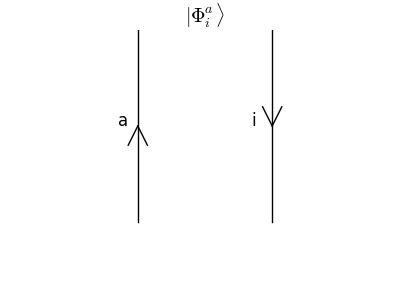
\includegraphics[width=0.5\textwidth]{diag_psi_ai}
    \caption{A Slater determinant with one hole state and one particle state.}
    \label{fig:diag_psi_ai}
\end{figure}

\begin{figure}[hbtp]
    \centering
    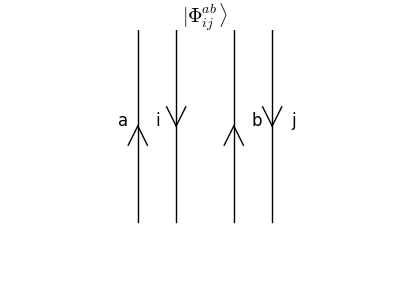
\includegraphics[width=0.5\textwidth]{diag_psi_aibj}
    \caption{A Slater determinant with two hole states and two particle states.}
    \label{fig:diag_psi_aibj}
\end{figure}

\FloatBarrier

\section{Operators}

We will use horizontal dashed lines to represent operators such as
terms in the normal-ordered hamiltonian. While the one-body operator
will have two lines entering and/or leaving, the two-body operator
will have four lines entering and/or leaving. The lines entering from
below represent the annihilation of pseudo particles, while lines
exiting above represent creation of pseudo particles. Following this
logic, we list the normal ordered one-body operator  of Eq.~(\ref{eqn:onebody_N}) 
and the normal ordered two-body operator
of Eq.~(\ref{fig:onebody}) diagrammatically, as shown in Figs.~\ref{fig:onebody},
\ref{fig:twobody1} and \ref{fig:twobody2}.
\begin{figure}[hbtp]
    \centering
    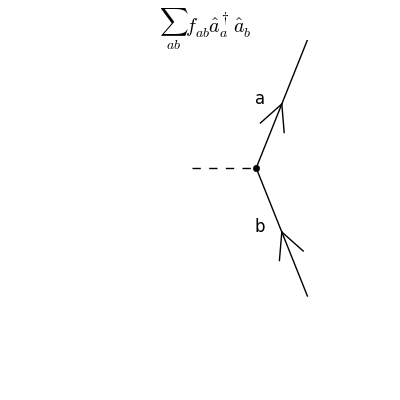
\includegraphics[width=0.4\textwidth]{onebody1}
    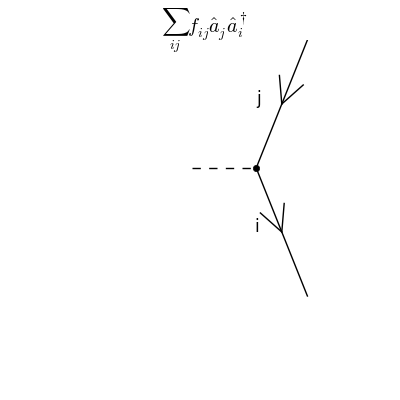
\includegraphics[width=0.4\textwidth]{onebody2}
    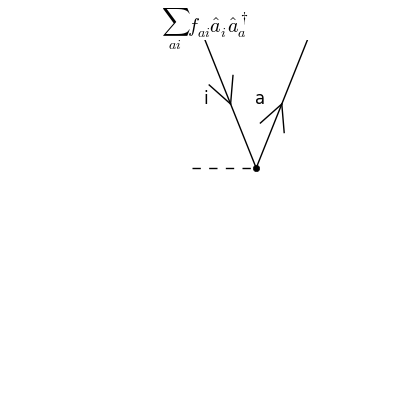
\includegraphics[width=0.4\textwidth]{onebody3}
    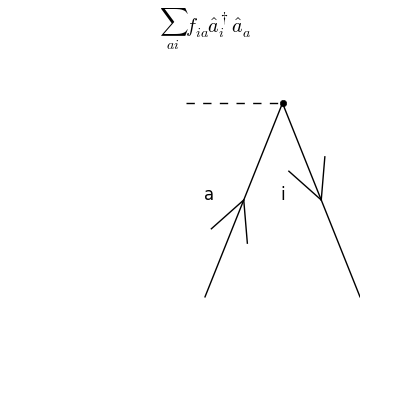
\includegraphics[width=0.4\textwidth]{onebody4}
    \caption{A normal ordered one-body operator with its mathematical expressions.}
    \label{fig:onebody}
\end{figure}

\begin{figure}[hbtp]
    \centering
    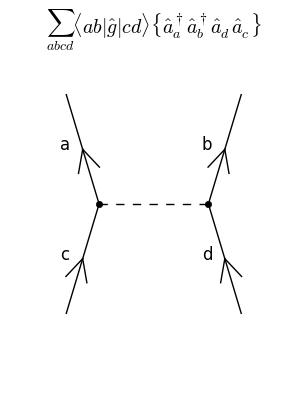
\includegraphics[width=0.4\textwidth]{twobody1}
    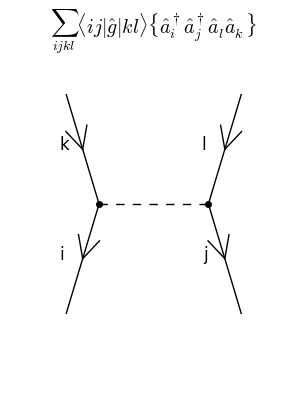
\includegraphics[width=0.4\textwidth]{twobody2}
    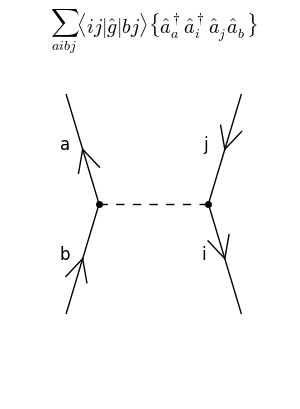
\includegraphics[width=0.4\textwidth]{twobody3}
    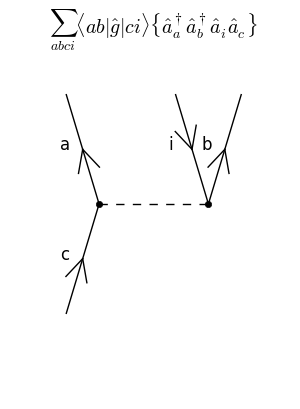
\includegraphics[width=0.4\textwidth]{twobody4}
    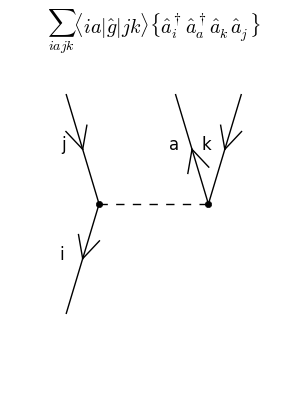
\includegraphics[width=0.4\textwidth]{twobody5}
    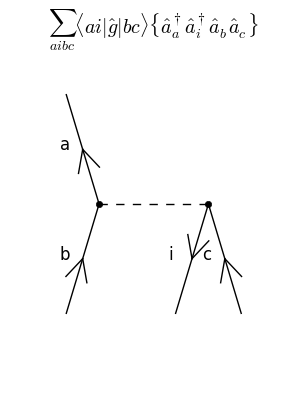
\includegraphics[width=0.4\textwidth]{twobody6}
    \caption{A normal ordered two-body operator with its mathematical expressions.}
    \label{fig:twobody1}
\end{figure}

\begin{figure}[hbtp]
    \centering
    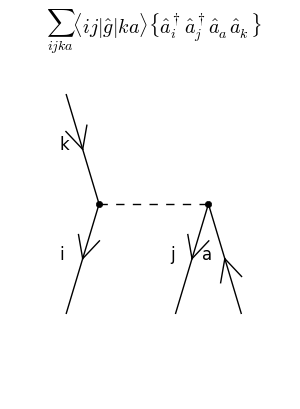
\includegraphics[width=0.4\textwidth]{twobody7}
    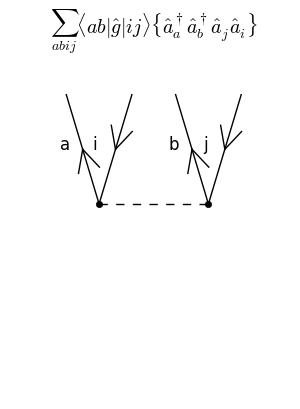
\includegraphics[width=0.4\textwidth]{twobody8}
    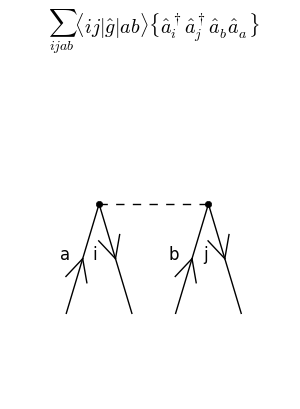
\includegraphics[width=0.4\textwidth]{twobody9}
    \caption{A normal ordered two-body operator with its mathematical expressions (continued).}
    \label{fig:twobody2}
\end{figure}

\FloatBarrier

\section{Contractions}

Diagrams allow us to represent contractions in a straight
forward manner, by connecting lines from Slater determinants to operators or between
operators. For example, we may consider the contraction of a singly
excited Slater determinants with a term in the normal ordered one-body operator, given by 
\begin{equation}
( \sum_{bc} f_{bc} \{  \Cr{b} \An{c} \}) \vert \Phi_i^a \rangle = ( \sum_{bc} f_{bc} \{ \Cr{b} \An{c} \})\{ \Cr{a} \An{i} \} \vert \Phi_0 \rangle = \sum_{bc} f_{bc} \delta_{ac}  \vert \Phi_i^b \rangle,
\label{eqn:onebody_N1}
\end{equation}
where the contraction occurs between the indices in the Kronecker delta, in terms of the  diagrammatic contraction 
performed in Fig. \ref{fig:contraction}.

\begin{figure}[hbtp]
    \centering
    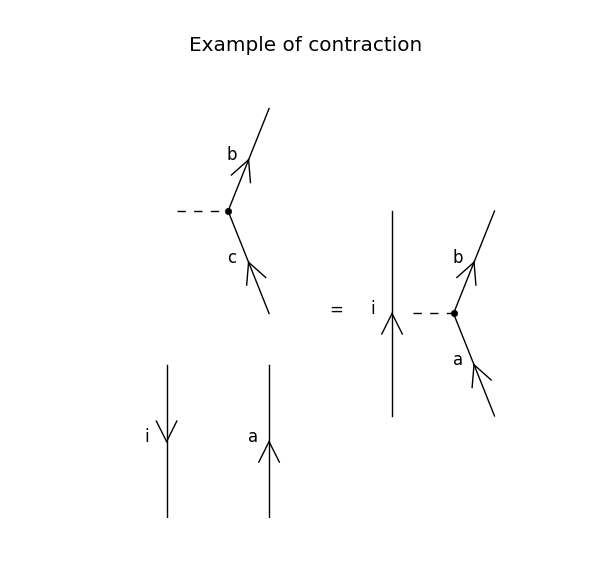
\includegraphics[width=0.7\textwidth]{contraction}
    \caption{A contraction of a one-body operator and a singly excited Slater determinant.}
    \label{fig:contraction}
\end{figure}

The diagrams resulting from this process may in turn be interpreted
back into mathematical expressions that we may use in implementations
of the various many-body methods.


\section{Interpreting diagrams}

The various many body methods which will be introduced in the upcoming
chapters rely on operator expressions and contractions. The basic idea
of using diagrams to derive such expressions may be outlined as
follows. For a given method we shall see that the contracted
expressions that are included in the  evaluation of say the correlation energy, may
be visually represented by a set of diagrams. The situation before
these contractions may also be visually represented by combinations of
such uncontracted vertices as shown in Figs. \ref{fig:twobody1}, \ref{fig:twobody2}, \ref{fig:onebody} (and so on). 

By defining consistent
rules for how the contracted diagrams are obtained from the
uncontracted vertices, we may skip the mathematical contraction
altogether, derive the various resulting terms, and interpret them
back into mathematical expressions by rules that ensure that all
factors and distinct features of the expressions are preserved.

Luckily, such consistent rules are present in the literature
\cite{ShavittBartlett2009} for many of the methods we discuss in the
upcoming chapter.
 %Diagrammatic notation

% Chapter Template

\chapter{Methodology} % Main chapter title

\label{Chapter4} % Change X to a consecutive number; for referencing this chapter elsewhere, use \ref{ChapterX}

\lhead{Chapter 5. \emph{Methodology}} % Change X to a consecutive number; this is for the header on each page - perhaps a shortened title

%----------------------------------------------------------------------------------------
%	SECTION 1
%----------------------------------------------------------------------------------------

\section{Many-body Methods}

As previously discussed in Chapter \ref{Chapter1}, the aim of many-body quantum mechanics 
is to find either the exact, or a reliable
approximation to the many-body systems wave function $\Psi$. In methods like coupled cluster theory, this wave
function resides in Fock space, a space spanned by all possible Slater
determinants constructed by the single-particle states from the
corresponding one-body problem. This wave function may be written (for
$N$ particles)
\begin{equation}
\vert \Psi \rangle = c_0 \vert \Phi_0 \rangle + \sum_{ai} c_{ai }\vert \Phi_i^a \rangle +  \sum_{abij} c_{abij} \vert \Phi_{ij}^{ab} \rangle + ... + \sum_{ab...N_a ij...N_i} c_{ab...N_a ij...N_i} \vert \Phi_{ij...N_i}^{ab...N_a} \rangle.
\label{eqn:fullCI}
\end{equation}

To determine the full wave function we therefore need a complete
single-particle basis as well as the means to project it onto Fock
space, determining its coefficients. In general, we may consider the
process of generating the full wave function from the reference state
to be an operator $\hat{\Omega}$ acting on the reference state
\begin{equation}
\vert \Psi \rangle = \hat{\Omega} \vert \Phi_0 \rangle .
\label{eqn:reference_operator}
\end{equation}

The explicit form of $\hat{\Omega}$ is to be determined by the various many-body methods. 

\section{The Hartree-Fock Method}

A complete basis often means an infinite number of single-particle
states, which in turn means an infinite number of Slater
determinants. Such a system is not possible to implement
computationally, so we may instead seek ways of truncating our
basis. As previously discussed in chapters 1 and 2, the precision of
our solution will now depend on how much of the exact wave function is
present in the retained basis. To this end, we will seek a
single-particle basis that ensures that most, or as much as possible,  of the systems wave
function is present in one single Slater determinant.

The \emph{Hartree-Fock method} is a way of optimizing the
single-particle states so that a single Slater determinant gives a
good representation of the system. The resulting Slater determinant
may serve as a starting point for several so called \emph{post Hartree-Fock methods}, 
such as MBPT (many body perturbation theory),
CI (Configuration Interaction) or CC (Coupled Cluster)
method \cite{ShavittBartlett2009}.

The first development of the method is attributed to Douglas Rayner
Hartree who in 1927 introduced a procedure he called 
\emph{the self  consistent field method} \cite{Thijssen} but which was later named
the \emph{Hartree-Fock-Rothaan} method. Some of the original differences between various Hartree-Fock approaches 
are nowadays seldomly mentioned or have simply been forgotten \cite{ShavittBartlett2009},
and the more generic name Hartree-Fock normally refers to the method that will be discussed in
the following sections.

\subsection{The variational principle}

The Hartree-Fock method is based on the variational principle, which
states that when we evaluate the inner product of the Hamiltonian on
\emph{any} normalized wave function, the resulting energy will be an
upper bound to the ground state energy \cite{Griffiths2005},
that is
\begin{equation}
E_0 \leq \langle \Psi_{trial} \vert \hat{H} \vert \Psi_{trial} \rangle.
\label{eqn:variational}
\end{equation}

Such wave functions are commonly called \emph{trial} wave functions. 

The variational principle provides us with an approximate scheme, and
by parameterizing the trial wave function we may improve upon this
solution.

\subsection{Expanding the single-particle states}

The parametrization of the Slater determinant may be performed by letting
each single-particle state be represented by a linear combination of
the eigenstates to the corresponding one-body problem. If we refer to
the linear combinations by $\psi$ with Latin indices and the basis
states as $\phi$ with Greek indices, we may write this as
\begin{equation}
\vert \psi_i \rangle = \sum_\alpha^A c_{\alpha,i} \vert \phi_{\alpha,i} \rangle .
\label{eqn:expanding_sp_states}
\end{equation}

Note that we truncate the basis at the A'th function to make
computations possible. More functions generally means a better
representation. In principle, our basis sets span an infinity of states, but due to obvious computational limits we have to truncate the above sum.

In accordance with the variational principle, we now want to determine
the coefficients $c_{\alpha, i}$ in such a way that we minimize the
energy. We should therefore insert the expanded single-particle states
into the energy equation (\ref{eqn:many_body_energy}) that we derived
in chapter 1. We will assume that the system's Hamiltonian has the form

\begin{equation}
\hat{H} = \hat{H}_0 + \hat{H}_I = \sum_{i=1}^N \hat{h}_0(\mathbf{x}_i) + \sum_{i<j=1}^N \hat{v}(\mathbf{x}_i,\mathbf{x}_j),
\end{equation}

where $N$ is the number of particles in our system,  $\hat{h}_0(\mathbf{x}_i)$ is the one body operator acting on particle $i$, and $\hat{H}_I$ is the interaction. For simplicity, we will avoid defining these in more detail, and we will use the following shorthand notation for the two-body integrals

\begin{equation}
\langle \alpha \beta \vert V \vert \alpha \beta \rangle \equiv \int \psi_\alpha^*(\mathbf{r}_i) \psi_\beta^*(\mathbf{r}_j) V(r_{ij})  \psi_\alpha(\mathbf{r}_i) \psi_\beta(\mathbf{r}_j) d\mathbf{r}_i\mathbf{r}_j,
\end{equation}

\begin{equation}
\langle \alpha \beta \vert V \beta \alpha \rangle \equiv \int \psi_\alpha^*(\mathbf{r}_i) \psi_\beta^*(\mathbf{r}_j) V(r_{ij})  \psi_\alpha(\mathbf{r}_j) \psi_\beta(\mathbf{r}_i) d\mathbf{r}_i\mathbf{r}_j,
\end{equation}

Where the quantity $r_{ij} = \vert \mathbf{r}_i - \mathbf{r}_j \vert$ indicates that the interaction depends upon the distance between the particles. We may even express this as an antisymmetric matrix element:

\begin{equation}
\langle \alpha \beta \vert V \vert \alpha \beta \rangle_{AS}  \equiv \langle \alpha \beta \vert V \vert \alpha \beta \rangle - \langle \alpha \beta \vert V \vert \alpha \beta \rangle.
\end{equation}

By inserting the expanded states in Eqn. \ref{eqn:many_body_energy}, we will find the eigenvalue of the Hamiltonian expressed as a function of the set of coefficients $\{c\}$
\begin{multline}
 \epsilon (\{c\}) = \sum _{\alpha, \beta}^A c_{\alpha,i}^{*}c_{\beta,i} \sum _{i}^N \langle \phi _\alpha | \hat{h}_0 | \phi _\beta \rangle + \\ 
 \sum _{\alpha,\beta, \gamma, \delta} ^A c_{\alpha,i}^{*}c_{\beta,j}^{*}c_{\gamma,i}c_{\delta,j}
 \frac{1}{2} \sum _{i=1,j=1}^N \langle \phi _{\alpha}\phi _{\beta}| \hat{v} |\phi _{\gamma}\phi _{\delta} \rangle_{AS}.
\label{eqn:greek_HF}
\end{multline}

The way in which we now have set up the system, we may consider the
coefficients to be a matrix with $A$ rows (Greek letters) and $N$
columns, where $N$ is the number of particles. In the special case
where diagonal elements are one and all others zero, we find the same
system as we have discussed up to this point.

\subsection{Ensuring orthonormality}

The trial wave function is now parameterized by the introduction of
coefficients. When varying or optimizing these coefficients to
minimize the energy, we must be careful to constrain the
orthonormality of the states (remember, failing to do so will cause a
violation of the Pauli principle). Mathematically this constraint may
be written
\begin{equation}
\langle \psi_i \vert \psi_j \rangle = \sum_{\alpha}^A c_{\alpha, i}^*c_{\alpha, j} = \delta_{ij}.
\label{eqn:orthonormality}
\end{equation}

To this end, we may use \emph{Lagrange's method of undetermined  multipliers} \cite[p.116]{Szabo} 
(or simply \emph{Lagrange  multipliers}), and set up a functional to be minimized with the
constraint described above, namely
\begin{equation}
 F\big( \epsilon \big( \{c\} \big), \lambda \big) =  \epsilon \big( \{c\} \big) - \sum _i^N \lambda _i \sum _{\alpha}^A c_{\alpha,i}^{*} c_{\alpha,i}.
 \label{lagrange_minim}
\end{equation}

To find a minimum for this functional we must solve
\begin{equation}
\frac{\partial}{\partial c_{\alpha,i}^{*}} F\big(  \epsilon \big( \{c\} \big), \lambda \big) = 0.
\label{eqn:partialset}
\end{equation}

For a step by step solution, the reader is referred to Thijssen's
\emph{Computational Physics} \cite{Thijssen} or Szabo's \emph{"Modern Quantum Chemistry"} \cite{Szabo}. 
In the following we will just
state the solution consistent with how it is given in these sources.

\subsection{The Hartree-Fock Equations}

By solving Eq.~(\ref{eqn:partialset}), we obtain a set of coupled one particle eigenvalue problems given by

\begin{multline}
\lambda _k c_{\alpha,k} =  
\sum _{\gamma}^A\sum _{i}^N c_{\gamma,k}\langle \alpha |\hat{h}_0| \gamma \rangle + 
\sum _{\beta,\gamma,\delta}^A \sum _i^N c_{\beta,i}^{*}c_{\gamma,i}c_{\delta,k}\langle \alpha \beta | V |\gamma \delta \rangle_{AS}.
 \label{eqn:HF1}
\end{multline}

These are known as the Hartree-Fock equations, and by identifying $\lambda$ as energy associated with single-particle state k \cite{hh4480} we may write them as
\begin{equation}
\epsilon_k^{HF} c_{\alpha,k} =  
\sum_{\gamma} \Big{(}  {\langle \alpha |\hat{h}_0 | \gamma \rangle + 
\sum_j^N \sum_{\beta \delta}{c_{j \beta} c_{j \delta}  \langle \alpha \beta | V | \gamma \delta \rangle_{AS} } } \Big{)} c_{ \gamma, k},
 \label{eqn:HF2}
\end{equation}

or simply 

\begin{equation}
\sum_\gamma f_{\alpha \gamma}^{HF} c_{\gamma,k} = \epsilon_k^{HF} c_{k,\alpha},
\label{eqn:hartreefock}
\end{equation}

where we defined

\begin{equation}
 f_{\alpha \gamma}^{HF}  \equiv   \langle \alpha |\hat{h}_0 | \gamma \rangle + 
\sum_j^N \sum_{\beta \delta}{c_{j \beta} c_{j \delta}  \langle \alpha \beta | V | \gamma \delta \rangle_{AS} } 
 \label{eqn:HF2}
\end{equation}

The matrix $ \hat{f}^{HF} $ is commonly known as the \emph{Fock}
matrix, and has dependence upon all the spin
orbitals. \cite{ShavittBartlett2009}. As a consequence, a first guess
for the coefficients is likely to be inconsistent when evaluating the
left hand side and right hand side of Eq.~(\ref{eqn:hartreefock}), so they
are normally solved in an iterative manner. This is why the method was
initially named the self-consistent field method; the field produced
by the particles should be consistent with the field "felt" by each
particle.

A set of single particle states that fulfills Eq.~(\ref{eqn:hartreefock})
are called the \emph{canonical Hartree-Fock wave function}, while the
constituent states are called \emph{the canonical spin orbitals}.

\subsection{Koopman's theorem}

The Hartree Fock energy for any single-particle state $p$ may be compactly written
\begin{equation}
\epsilon^{HF}_p = \langle p \vert \hat{h}_0 \vert p \rangle + \frac{1}{2} \sum_{j} \langle pj \vert  \vert pj \rangle .
\label{eqn:hf_koopman}
\end{equation}

This is the energy associated with each orbital expanded as a linear combination of single-particle states. Each fermion in the system will then have an associated Hartree-Fock energy.

Koopman's theorem states that for closed-shell Hartree-Fock
calculations, the ionization energy of the system is equal to the
negative of the outermost hole state in the reference state. \cite{Thijssen}
The ionization energy may then be computed by performing a Hartree-Fock procedure, 
whereby we calculate only the outermost occupied
orbital in equation Eq.~(\ref{eqn:hf_koopman}).

\subsection{Restricted and unrestricted Hartree-Fock}

There are multiple ways of implementing the Hartree-Fock
equations. For closed shell systems, such as $He$, $H_2$ and $Be$, the
electrons (we consider only electronic degrees of freedom in this thesis), may be assumed to be paired with
opposite spin electrons. In the restricted Hartree-Fock method (RHF),
we consider only systems where all fermions (electrons in our case) are paired with opposite
spin particles. This lets us scale down the computation, but it will
naturally give poor results for systems where no such pairing occurs,
for example in the case where two $H$ atoms are interacting over
large distances.

For systems with singly occupied states (unpaired fermions, typically
odd numbered systems) the restriction of spin-pairing is no longer valid.

To take this into account, we set up two Fock matrices; one for each
spin orientation. The resulting system is
\begin{equation}
\hat{F}_\alpha(C_\alpha, C_\beta) C_\alpha = \hat{S} C_\alpha \epsilon_\alpha,
\end{equation}
and
\begin{equation}
\hat{F}_\beta(C_\alpha, C_\beta) C_\beta = \hat{S} C_\beta \epsilon_\beta.
\end{equation}

The subindices $\alpha$ and $\beta$ makes the distinction between the two possible spin-orientations in our system, for example $\alpha$ for spin up and $\beta$ for spin down. For each orientations we have a separate coefficient matrix $C$.

The ground state energy will be a function of the eigenvectors of
these two matrices. The dependency of opposite spin coefficients in
the Fock matrices is due to the direct- or coulomb term from the two
particle integrals \cite[p.241]{Szabo}. This latter approach is called
the \emph{unrestricted Hartree-Fock} (UHF) method.



\section{Post Hartree-Fock Methods}

While the Hartree-Fock reference state may account for important
correlations such as the Pauli exclusion principle and interactions
with the mean field, it will lack the more complicated correlations. For this reason, certain correlations may never
be fully accounted for with the Hartree-Fock method alone. Figure
\ref{fig:correlation} illustrates what is often defined as the
correlation energy; the energy attributed to correlations beyond the
mean field.
\begin{figure}[p]
    \centering
    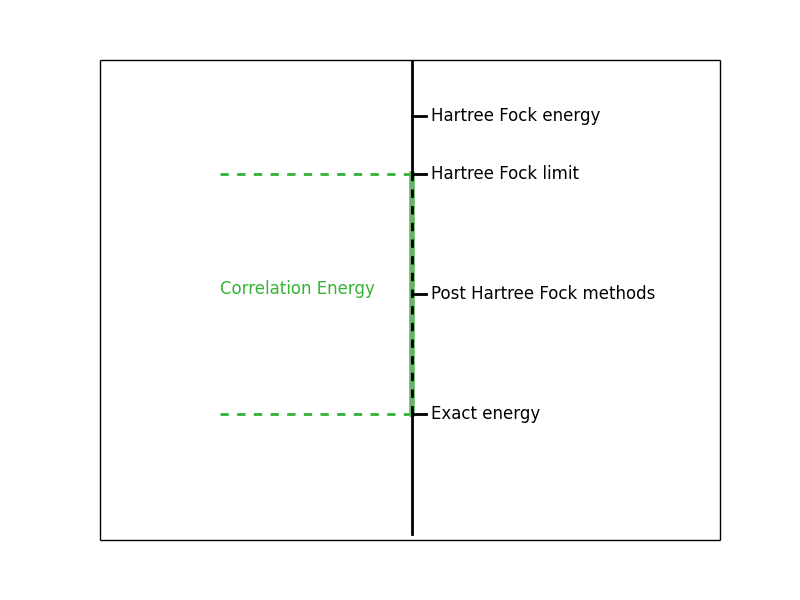
\includegraphics[width=0.8\textwidth]{correlation}
    \caption{Correlations beyond the Hartree-Fock energy. At the so
      called Hartree-Fock limit, we have achieved the best possible
      description of our system using the mean field approach. The
      energy unaccounted for by the reference state is commonly
      referred to as the \emph{correlation energy}. The so called
      \emph{post Hartree-Fock} methods, such as the Coupled Cluster
      method, will help us include even more correlations and bring us
      closer to the exact energy.}
    \label{fig:correlation}
\end{figure}

A Hartree-Fock calculation may also provide us with energy minimized orbitals above the Fermi level that may be used to construct excited Slater determinants in so-called \emph{post Hatree Fock} methods. 

By including excited Slater determinants, these methods may
account for the correlations beyond the mean field. One such approach is the Coupled Cluster (CC) method, which
is a central subject in this thesis. Alongside CC, we have several
other methods such as Configuration Interaction (CI) or Many Body
Perturbation Theory (MBPT).

Important insight into various physical systems may be gained by
comparing results amongst these methods, as they all have their
strengths and weaknesses. Prior to the treatment of the CC method in
chapter 5, we shall therefore just briefly discuss some of these
alternative post Hartree-Fock methods, allowing us to make a meaningful comparison of
results in the final chapter of this thesis.

\subsection{Configuration Interaction theory}

The Configuration Interaction (CI) method, sometimes referred to as
the \emph{method of superposition of configurations} \cite{Harris} is
based on the expansion of the system's wave function into a linear
combination consisting of the reference Slater determinant and a
(possibly infinite) set of excited versions of this Slater
determinant, as briefly noted in the introduction to this chapter,
\begin{equation}
\vert \Psi \rangle = c_0 \vert \Phi_0 \rangle + \sum_{ai} c^{a}_i\ vert \Phi_i^a \rangle +  \sum_{abij} c^{ab}_{ij} \vert \Phi_{ij}^{ab} \rangle + ... + \sum_{ab...N_a ij...N_i} c^{ab...N_a}_{ij...N_i} \vert \Phi_{ij...N_i}^{ab...N_a} \rangle.
\label{eqn:fullCI}
\end{equation}

The CI method is considered to be the mathematically simplest
technique for inclusion of correlations beyond the mean
field \cite{Harris}. The operator that brings us from the reference
Slater determinant to the true system wave function may be written
\begin{equation}
\vert \Psi \rangle = \Omega \vert  \Phi_0 \rangle = (c_0 + \hat{C}) \vert  \Phi_0 \rangle,
\end{equation}
where
\begin{equation}
\hat{C} = \sum_{ai} c^{a}_i \Cr{a} \An{i}+  \sum_{abij} c^{ab}_{ij} \Cr{a} \Cr{b} \An{j} \An{i} + ... + \sum_{ab...N_a ij...N_i} c^{ab...N_a}_{ij...N_i} \Cr{a} \Cr{b} ... \Cr{N_a} \An{N_i} ... \An{j} \An{i}.
\end{equation}

The coefficients $c$ are then obtained by diagonalization, which corresponds to  minimizing 
\begin{equation}
E = \langle \Psi \vert \hat{H} \vert \Psi \rangle.
\label{eqn:fullCIvar}
\end{equation}

We shall not go into more details concerning this. The reader is
referred to for example \cite[p.177]{Harris} for a more complete
treatment.

We will however make some general observations concerning the CI method. 

\subsection{Full Configuration Interaction theory}

Equation (\ref{eqn:fullCIvar}) is solvable, but at great
computational cost. The number of excited Slater determinants, and
thereby the number of coefficients, scales \emph{factorially} with the
number of particle states and hole states.

The practical consequence is that the inclusion of all Slater
determinants is only possible for smaller systems unless some
truncation in the basis set is introduced. From a physical
point of view, we may have systems where no single excitation is
allowed, and for this reason the singly excited coefficients may be
excluded with no loss of precision.

The various truncations are commonly referred to as CIS for inclusion
of single excitations, CISD for single and double excitations and so
on.

\subsection{Configuration Interaction Quantum Monte Carlo}

We will later in this thesis compare results with results from a
so-called FCIQMC (Full Configuration Interaction Quantum Monte Carlo)
calculation. This approach determines the FCI coefficients by
stochastic processes \cite{Booth2013,Leikanger2013}. Such
results are valuable for our purpose, since they basically provide us
with the exact ground state energy for smaller systems, which will
allow us to evaluate to which degree the method accounts for
correlations in the system.

\subsection{Many Body Perturbation Theory}

As opposed to the Hartree-Fock, Configuration Interaction and
Coupled Cluster methods, \emph{Many Body Perturbation Theory} (MBPT)
offers a non-iterative approach to approximating the systems wave
function. The following derivation is based on the one in Refs.
\cite{ShavittBartlett2009} and \cite{hh4480}.

The basic idea is to arrange the Hamiltonian into two parts
\begin{equation}
\hat{H} = \hat{H}_0 + \hat{V}.
\end{equation}

This is very similar to what we have done so far, as we seek an
operator $\hat{H}_0$ which is exactly solvable (which yields the
single-particle basis) and an operator $\hat{V}$ that will be treated as a
perturbation. The solution to the unperturbed problem is given
\begin{equation}
\hat{H}_0 \vert \Phi_0 \rangle = W_0 \vert \Phi_0 \rangle.
\end{equation}

As for Configuration Interaction theory, we have the exact ground state wave
function for our system represented by a linear combination of Slater
determinants, where we assume the first term (reference state) to be
the dominating term
\begin{equation}
\vert \Psi_0 \rangle = \vert \Phi_0 \rangle + \sum_m^\infty c_m \vert \Phi_m \rangle.
\end{equation}
 
We then assume intermediate normalization $\langle \Phi_0 \vert
\Psi_0 \rangle = 1$ and project our Schödinger equation onto $\langle
\Phi_0 \vert$ :
\begin{equation}
\langle \Phi_0 \vert \hat{H} \vert \Psi_0 \rangle = \langle \Phi_0 \vert \hat{H}_0 + \hat{V} \vert \Psi_0 \rangle = E.
\end{equation}

The true ground state energy is still unknown, but we
may subtract the \emph{unperturbed} energy to find an expression for
the correlation energy
\begin{equation}
\langle \Phi_0 \vert \hat{V} \vert \Psi_0 \rangle = E - W_0 = \Delta E.
\end{equation}

We may add and subtract a term $\omega \vert \Psi_0 \rangle$ to the expression above and regroup it to find
\begin{equation}
\vert \Psi_0  \rangle = \frac{1}{(\omega - \hat{H}_0)} (\hat{V} + \omega - E) \vert \Psi_0 \rangle .
\label{eqn:pt_1}
\end{equation}

By interpreting the term $\omega$ in different ways, we will arrive at the various many-body perturbation schemes.

The system's true wave function is still unknown, but it is fully
possible to expand it in a known basis $\{\phi_n \}$, so that
\begin{equation}
\vert \Psi \rangle = (\hat{P} + \hat{Q})\vert \phi_0 \rangle,
\end{equation}
where we have the projection operator $\hat{P} = \vert \phi_0 \rangle \langle \phi_0 \vert$, $\hat{P} = \hat{P}^\dagger = \hat{P}\hat{P}$ and $\hat{Q} = \sum_{m} \vert \phi_m \rangle \langle \phi_m \vert$ \cite{ShavittBartlett2009}. 
We insert this into Eq. (\ref{eqn:pt_1}) to find
\begin{equation}
\vert \Psi_0  \rangle = \phi_0 \rangle + \sum_i^\infty \Big{(} \frac{1}{(\omega - \hat{H}_0)} (\hat{V} + \omega - E) \Big{)}^i \vert \phi_0 \rangle ,
\label{eqn:pt_2}
\end{equation}
and the correlation energy takes the form
\begin{equation}
\Delta e = \sum_i^\infty  \hat{V} \Big{(} \frac{1}{(\omega - \hat{H}_0)} (\hat{V} + \omega - E) \Big{)}^i \vert \phi_0 \rangle .
\label{eqn:pt_2}
\end{equation}

By letting $\omega = E$, we obtain the so called Brillouin-Wigner
Perturbation Theory, or we may let $\omega = W_0$ to obtain
Rayleigh-Schrödinger Perturbation Theory (RSPT). In the
Brillouin-Wigner case, a possible solution would involve iterations
and self consistence as in the Hartree-Fock-, Configuration Interaction- and Coupled Cluster cases, while in the RSPT
case we end up with terms that correspond to different orders of the
correlation energy. For RSPT, we obtain
\begin{equation}
\Delta e = \Delta E^{(1)}+\Delta E^{(2)}+\Delta E^{(3)}+... ,
\end{equation}
where
\begin{equation}
\Delta E^{1} = \langle \phi_0 \vert \hat{V} \vert \phi_0 \rangle,
\end{equation}
\begin{equation}
\Delta E^{2} = \langle \phi_0 \vert \hat{V}  \frac{\hat{Q}}{(W_0 - \hat{H}_0)}  (\hat{V} - \Delta E) \vert \phi_0 \rangle,
\end{equation}
\begin{equation}
\Delta E^{3} = \langle \phi_0 \vert \hat{V} \frac{\hat{Q}}{(W_0 - \hat{H}_0)}  (\hat{V} - \Delta E) \frac{\hat{Q}}{(W_0 - \hat{H}_0)}  (\hat{V} - \Delta E)  \vert \phi_0 \rangle,
\end{equation}
represent the correlation energy to first, second and third order, respectively. Higher orders are obtained along similar lines. Every order in RSPT introduces different types of correlations. With a two-body force only, to second order we can obtain contributions from at most two-particle-two-hole excitations. At for example fourth order, we can also obtain contributions
which represent four-particle-four-hole  excitations.  
Whereas methods like Configuration Interaction or Coupled Cluster include such correlations 
to infinite order in the interaction, RSPT contains such correlations only up to the given order in the expansion.



\subsection{The linked diagram theorem}

We will not go into any further detail on the many-body perturbation
methods, but we should note an important theorem introduced by
Goldstone \cite{Goldstone1957}, see also Ref.~\cite[p.152]{ShavittBartlett2009}.

Computations of the different orders in Rayleigh-Schrödinger
Perturbation Theory may be performed diagrammatically. Based on a set
of rules (see for example \cite{ShavittBartlett2009}), we may generate
diagrams corresponding to the possible contractions operators
present in each order of the perturbation. Actually, the diagrammatic
rules will produce a lot more diagrams then what is actually needed in
order to calculate the correlation energy.

The \emph{linked diagram theorem} is a simple way of getting rid of a lot of these excess diagrams.

A diagram may be called \emph{linked} if all parts of the diagram is
linked with each other by contractions. Unlinked diagrams will be
easily identified as it is possible to split them into smaller parts
by drawing lines through them without crossing any lines in the
diagram.

The linked diagram theorem states that these diagrams do not contribute to the correlation energy. 

In Eq. (\ref{eqn:pt_2}) for Rayleigh-Schrödinger Perturbation Theory, we will therefore only have to consider terms where contractions occur for diagrams where every vertex is linked to another vertex by at least one particle or hole line.

\section{Other many-body methods}

The methods we have discussed so far are relevant to this thesis, but the full range of methods for dealing with many body problems extends even further. Some notable methods apart from the ones discussed so far is the wide range of \emph{Quantum Monte Carlo} (QMC) methods, that build upon the same formalism as us, but use instead stochastic methods to approximate the systems wavefunction (see for example \cite[Chapter 12]{Thijssen}). Other methods such as \emph{Density Functional Theory} (DFT) may even depart from the Hartree-Fock formalism to offer more suitable equations for solids, while at the same time represent alternatives to Hartree-Fock calculations for atoms and molecules \cite[Chapter 5]{Thijssen}.  %Methodology
% Chapter Template

\chapter{The Coupled Cluster Method} % Main chapter title

\label{Chapter5} % Change X to a consecutive number; for referencing this chapter elsewhere, use \ref{ChapterX}

\lhead{Chapter 6. \emph{The Coupled Cluster Method}} % Change X to a consecutive number; this is for the header on each page - perhaps a shortened title

%----------------------------------------------------------------------------------------
%	Introduction
%----------------------------------------------------------------------------------------

\section{Historical Account}


As is the case with many contributions to science, it is hard to
pinpoint the origin of the Coupled Cluster methods to one single
scientific work. It is however commonly accepted that the groundbreaking
work was made by the nuclear physicists Fritz Coester and
Hermann Kümmel in the mid and late 50s. At this time the computational aspects
of many body theory was still in its early infancy, although some
variational Hartree-Fock calculations had been performed in the
quantum chemistry community. \cite{Kummel}

One important discovery that may have motivated work on the Coupled
Cluster method was made by J. Hubbard, who laboriously inspected the
time independent perturbation series to all orders and found that only
linked terms contribute to the energy, as well as that the energy
associated with these terms was \emph{extensive} \cite{Hubbard}.

Coester was then shortly after the work of Hubbard able to derive
basically the same results using the \emph{exponential ansatz} and
\emph{the Hausdorff expansion} \cite{Kummel}. In the following years,
Kümmel and Coester published a number of papers describing the method \cite{Coester1958, Coester1960b},
and by the late 1950s the method was well understood \cite{Kummel}.

Together with Haag, Coester was also able to show that the
exponential ansatz was a natural choice for the system's wave function
\cite{Coester1960a}, meaning that the choice was not as arbitrary as one may get
the impression of when reading modern books on the
subject \cite{ShavittBartlett2009}.


Despite this, it was not until 1966 that the first real applications
of the method were made, and these were made by the quantum chemist Jiri
Cizek \cite{Cizek1966}. Coupled Cluster calculations for nuclear
matter were performed in the late 1970s and early 1980s \cite{kummel1978,day1981}.

Today, the so called Hartree-Fock + CCSD(T) (Coupled Cluster Singles
Doubles and Perturbative Triples) calculation is considered the "gold
standard" of quantum chemistry, due to its relatively low
computational cost compared to its ability to account for important
correlations in many systems.


\section{The exponential ansatz}
The derivation of the coupled cluster method begins with assuming that
the operator that brings the reference state into the true system
state can be represented by the exponetial operator
\begin{equation}
e^{\hat{T}} ,
\label{eqn:exponential_ansatz}
\end{equation}
where the \emph{cluster operator} is defined as
\begin{equation}
\hat{T} \equiv  \hat{T}_1 + \hat{T_2} + ... = 1 + \sum_{ai} t_i^a a_{a}^\dagger a_i + \sum_{ai} t_{ij}^{ab} a_{a}^\dagger a_{b}^\dagger a_i a_j + ...
\end{equation}

As may be seen from the second quantized form of the cluster operator,
its terms will cause an excitation of the reference state. For
example, the excitation operator $\hat{T}_1$ generates  a singly
excited reference state
\begin{equation}
\hat{T}_1\vert \Phi_0\rangle = \sum_{ai} t_i^a a_{a}^\dagger a_i|\Phi_0\rangle = \sum_{ai} t_i^a \vert \Phi_i^a\rangle,
\end{equation}
while the $\hat{T}_2$ operator creates a doubly excited reference state
\begin{equation}
\hat{T}_2 \vert \Phi_0\rangle = \sum_{abij} t_{ij}^{ab} a_{a}^\dagger a_{b}^\dagger a_i a_j|\Phi_0\rangle = \sum_{abij} t_{ij}^{ab} \vert \Phi_{ij}^{ab}\rangle,
\end{equation}
and so on. 

For reasons that will become clear shortly, there is no need to
include excitation operators beyond $\hat{T}_4$ for systems containing
at most two-body interactions. Truncations in the cluster operator are
commonly made to give rise to the different types of coupled cluster
methods.

The coefficients $t^{ab..}_{ij...}$ are commonly referred to as \emph{amplitudes}, and they are the quantities whose solution we will seek in an iterative way.

As for any exponential function, we may expand it as
\begin{equation}
e^{\hat{T}} = 1 + \hat{T} + \frac{1}{2!} \hat{T}^2 + \frac{1}{3!} \hat{T}^3 + ... ,
\end{equation}
meaning that  the exponential ansatz may be written
\begin{equation}
e^{\hat{T}}  \vert \Psi_0 \rangle = (1 + \hat{T} + \frac{1}{2!} \hat{T}^2 + \frac{1}{3!} \hat{T}^3 + ...) \vert \Psi_0 \rangle .
\end{equation}

\section{Size consistency}
The concept of size consistency was introduced by Pople {\em et al.} in 1978
\cite{Pople} to describe methods that properly represent systems in
the noninteracting limit. A system of electrons interacting through
the Coulomb force has a noninteracting limit when the distance
between the electrons is so large that the energy of this
configuration should correspond to the energy of an equal number of
noninteracting electrons.

In other words, a size consistent method should for the interacting
systems A and B produce energy calculations in the noninteracting
limit where \cite[p.12]{ShavittBartlett2009}
\begin{equation}
E(AB) = E(A) + E(B)
\end{equation}

Because of the fundamental assumption of pairing of electrons in the
restricted Hartree-Fock (RHF) method, this method is not size consistent for
systems such as the $H_2$ molecule. This shortcoming may however be
mended by performing a coupled cluster calculation on top of the RHF,
producing size consistent energies when gradually separating the
hydrogen nucleis (and their electrons). This is illustrated by a
comparison of RHF, unrestricted Hartree-Fock (UHF) and RHF+CCSD (coupled cluster theory at the level of singles and doubles excitations only) 
for the $H_2$ molecule in Fig.
\ref{fig:uhf_rhf_ccsd_h2}. It is clear that since the RHF method forces the
electrons of each hydrogen atom to pair, the energy is wrongly estimated
compared to the exact energy as we separate the hydrogen nuclei. 

By performing a CCSD calculation employing  the RHF basis, this restriction is lifted, allowing the
electrons to fall into their natural orbits. An unrestricted Hartree-Fock calculation on the other hand does
not assume the electrons to be paired, allowing thereby for a natural
behavior as the separation in distance between the two hydrogen nuclei increases.


\begin{figure}[hbtp]
    \centering
    \includegraphics[width=0.8\textwidth]{uhf_rhf_ccsd_h2}
    \caption{Comparison of UHF, RHF and RHF+CCSD for a $H_2$
      molecule. These results were produced by the author using a self-developed 
      solver \cite{FermionMingle} that utilizes gaussian
      basis sets to enable RHF, UHF, CCD and CCSD calculation on atoms
      and molecules. These results
      illustrate the size consistency of the CCSD equations, and
      the lack of size consistency in the RHF case. The vertical
      jumps in the curves are regions where the solver failed to
      converge due to improperly chosen relaxation parameters. Central parts of the code \cite{FermionMingle} that was used to produce these calculations was developed by the author as part of another course.}
    \label{fig:uhf_rhf_ccsd_h2}
\end{figure}


When comparing CC with CI, we will find that the $\hat{C}_2$ operator
has a corresponding combination of cluster operators
\begin{equation}
\hat{C}_2 = \hat{T}_2 + \frac{1}{2}(\hat{T}_1)^2.
\end{equation} 
The last quadratic term above is commonly referred to as a
\emph{disconnected cluster}, and such terms are responsible for
ensuring the consistency of the CC method.



\section{Extensivity}

A related concept to consistency is \emph{size extensivity}, as
introduced by Bartlett \cite{Bartlett1981}. A quantum mechanical model
may be called \emph{extensive} if the energy of this model scales
correctly with the size of the
system \cite[p.11]{ShavittBartlett2009}. This is analogous to
extensive properties in statistical mechancial systems, that scales
linearly with the size of the system, see for example Ref.~\cite[p.9]{Linder}.

When performing calculations on periodic systems such as gases or
solids, extensivity is a feature that allows us to extrapolate results
beyond the limits of the simulation cell.

For the coupled cluster method, extensivity is an inherent property of
the exponential ansatz (see Eq. (\ref{eqn:exponential_ansatz})). This may be shown
by considering that the reference state is separable, implying that
\begin{equation}
\phi_0(A,B) = \phi_0(A)\phi_0(B).
\end{equation}

Furthermore, the cluster operators are additive and we have
\begin{equation}
\hat{T}(A,B) = \hat{T}(A) + \hat{T}(B) .
\end{equation}

It then follows that the total wave function is multiplicatively separable
\begin{equation}
\Psi(A,B) = e^{T(A) + T(B)}\phi_0(A,B) = e^{T(A)}\phi_0(A)e^{T(B)}\phi_0(B).
\end{equation}

Thus, the energy is additive:
\begin{equation}
\hat{H}(A,B)\Psi(A,B) = [E(A) + E(B)]\Psi(A,B).
\end{equation}


\section{Deriving the coupled cluster equations}

We will derive the coupled cluster equations in four steps. First we
shall do some more work on the exponential ansatz to derive a form
that is more easily translated to actual calculations, secondly we
will introduce diagrammatic rules that will simplify derivations
considerably, and then we shall briefly comment upon how to translate
these rules into a code that makes the process of deriving coupled
cluster equations (and code) of any order remarkably simple.

Since the actual equations that are worked into a high-performance code
will depend upon how we truncate the ansatz, we will then finally
derive the full equations using the above mentioned code in increasing
order of complexity.

\section{Unwrapping the exponential ansatz}

\subsection{The CC effective Hamiltonian}

The actual quantity we seek is the correlation energy $\Delta e$ as
found by solving the Schrödinger equation for the exponential ansatz
and the normal ordered Hamiltonian Eq.~(\ref{eqn:hamiltonian_N})
\begin{equation}
\hat{H}_N e^{\hat{T}} \vert \Phi_0 \rangle =  \Delta e  e^{\hat{T}} \vert \Phi_0 \rangle.
\end{equation}
We may reorganize this into
\begin{equation}
(\hat{H}_N - \Delta e) e^{\hat{T}} \vert \Phi_0 \rangle = 0.
\end{equation}
By multiplying with the inverse exponential, we find
\begin{equation}
(e^{\hat{-T}} \hat{H}_N e^{\hat{T}} - \Delta e)  \vert \Psi_0 \rangle = 0,
\label{eqn:cc1}
\end{equation}
where the non-Hermitean operator
\begin{equation}
e^{\hat{-T}} \hat{H}_N e^{\hat{T}}  \equiv \mathcal{H},
\end{equation}
is a similarity transformed Hamiltonian, often called the \emph{CC effective Hamiltonian}.

By projecting Eq.~(\ref{eqn:cc1}) onto the reference state, we may then solve for the correlation energy
\begin{equation}
\langle \Phi_0 \vert e^{\hat{-T}} \hat{H}_N e^{\hat{T}} \vert \Psi_0 \rangle = \Delta e.
\label{eqn:cc2}
\end{equation}

It also follows that
\begin{equation}
\langle \Phi^* \vert e^{\hat{-T}} \hat{H}_N e^{\hat{T}} \vert \Psi_0 \rangle = 0,
\label{eqn:cc2}
\end{equation}
where $\Phi^*$ represents any excited state. This last equation will aid us in solving the amplitudes.

\subsection{Non-variational coupled cluster theory}

At this point we should note that the CC effective Hamiltonian is no longer Hermitean, since
\begin{equation}
\mathcal{H}^\dagger = (e^{\hat{-T}} \hat{H}_N e^{\hat{T}})^\dagger = (e^{\hat{-T}})^\dagger \hat{H}_N (e^{\hat{T}})^\dagger = (e^{\hat{-T^\dagger}}) \hat{H}_N (e^{\hat{T^\dagger}}) \neq \mathcal{H}
\end{equation}

A consequence is that truncations in the cluster operator will cause
the energy expression in Eq. (\ref{eqn:cc2}) to no longer be
variational, and thus the energy does no longer represent an upper
bound to the ground state energy \cite{CrawfordSchaefer}. In practice,
however, solving the resulting equations obtained from the
projection technique in Eq.~(\ref{eqn:cc2}) will still provide us
with an energy close to the real expectation value even for truncated
cluster operators \cite{CrawfordSchaefer}.

\subsection{The Hausdorff Expansion}

The Hausforff expansion (or Baker-Campbell-Hausdorff formula) provides
us with the means of rewriting the CC effective Hamiltonian in terms
of nested commutators \cite[p.293]{ShavittBartlett2009}:
\begin{equation}
\mathcal{H} = \hat{H}_N + [\hat{H}_N, \hat{T}] + \frac{1}{2} [[\hat{H}_N, \hat{T}], \hat{T}] +  \frac{1}{3!} [[[\hat{H}_N, \hat{T}], \hat{T}], \hat{T}] + \frac{1}{4!} [[[[\hat{H}_N, \hat{T}], \hat{T}], \hat{T}], \hat{T}].
\end{equation}

The reason that this sum of nested operators truncates at the
four-fold commutator, will become apparent if we use Wicks generalized
theorem to evaluate the expansion. For two strings of evenly numbered
creation- and annihilation operators, we will find the commutator
\begin{equation}
[A,B] = AB - BA = np[A,B] + 
\contraction{}{A}{}{B}
AB - np[B,A] - 
\contraction{}{B}{}{A}
BA,
\end{equation}
where the contraction represents the sum of all normal ordered products with one or more contractions present. 

This is simplified further since both $A$ and $B$ (in our case $H$ and
$T$) contain an even number of creation and annihilation operators
\begin{equation}
np[A,B] = np[B,A],
\end{equation}
meaning that  the uncontracted normal ordered products cancel
\begin{equation}
[A,B] =  
\contraction{}{A}{}{B}
AB - 
\contraction{}{B}{}{A}
BA.
\end{equation}
Since the cluster operators $T_m$ commute, the nested operators will
only have surviving terms where $\hat{H}_N$ contracts with one or more
cluster operators.

The reason for the truncation of the Hausdorff expansion is then
apparent; $\hat{H}_N$ is a sum of operators which at most contains
four creation or annihilation operators. It is therefore not possible
to contract any term in $\hat{H}_N$ to more than 4 cluster operators
as long as the Hamiltonian contains at most two-body interactions.

\subsection{Rewriting the Hausdorff expansion}

We also have to take into account that particle creation operators can
only produce a nonzero contraction with a particle annihilation
operator to its left, and a hole annihilation operator may only
produce a nonzero contraction with a hole creation operator to its
left, meaning that the only contributing terms when computing the nested
operator are terms that begin with the normal ordered Hamiltonian
\begin{equation}
\mathcal{H} = e^{\hat{-T}} \hat{H}_N e^{\hat{T}} = 
\hat{H}_N + 
\contraction{}{\hat{H}_N}{}{\hat{T}}
\hat{H}_N \hat{T} + 
\contraction{}{\hat{H}_N}{}{\hat{T}}
\contraction{}{\hat{H}_N}{\hat{T}}{\hat{T}}
\frac{1}{2} \hat{H}_N \hat{T} \hat{T} +
\contraction{}{\hat{H}_N}{}{\hat{T}}
\contraction{}{\hat{H}_N}{\hat{T}}{\hat{T}}
\contraction{}{\hat{H}_N}{\hat{T} \hat{T} }{\hat{T}}
\frac{1}{3!} \hat{H}_N \hat{T} \hat{T} \hat{T}  +
\contraction{}{\hat{H}_N}{}{\hat{T}}
\contraction{}{\hat{H}_N}{\hat{T}}{\hat{T}}
\contraction{}{\hat{H}_N}{\hat{T} \hat{T} }{\hat{T}}
\contraction{}{\hat{H}_N}{\hat{T} \hat{T} \hat{T} }{\hat{T}}
\frac{1}{4!} \hat{H}_N \hat{T} \hat{T} \hat{T} \hat{T} \equiv
(\hat{H}_Ne^{\hat{T}})_C
\label{eqn:hausdorff2}
\end{equation}

The contractions indicate a sum over all terms in which the
Hamiltonian connects by at least one contraction to each of the cluster
operators to its right. The subscript C indicates connected
terms only. For further details, see Ref.~\cite[p.294]{ShavittBartlett2009}.

\subsection{The CC equations}

We are finally in a position to derive explicit expressions for the energy and amplitudes.
We have the general equation 
\begin{equation}
(\hat{H}_Ne^{\hat{T}})_C \vert \Phi_0 \rangle = \Delta e \vert \Phi_0 \rangle.
\end{equation}
Finding the energy is now simple, we have
\begin{equation}
\langle \Phi_0 \vert (\hat{H}_Ne^{\hat{T}})_C \vert \Phi_0 \rangle = \Delta e  .
\label{eqn:ccm1}
\end{equation}

The amplitudes may be found from the equations 
\begin{equation}
\langle \Phi_i^a \vert (\hat{H}_Ne^{\hat{T}})_C \vert \Phi_0 \rangle = 0  ,
\label{eqn:ccm2}
\end{equation}
and
\begin{equation}
\langle \Phi_{ij}^{ab} \vert (\hat{H}_Ne^{\hat{T}})_C \vert \Phi_0 \rangle = 0 ,
\label{eqn:ccm3}
\end{equation}

and so on, depending on how we truncate the cluster operator. We will
refer to the first equation (\ref{eqn:ccm1}) 
as the \emph{energy  equation}, while the following ones will be referred to as the
\emph{amplitude equations}.

\subsection{Truncating the ansatz}

The connection requirements of the CC effective Hamiltonian in
Eq. (\ref{eqn:hausdorff2}) will also impact on truncations in the
cluster operator. Since our Hamiltonian at most contains four pairs of
creation- and annihilation operators (that is we at most a two-body interaction), 
it will not be able to fully
contract with cluster operators beyond the four-fold excitation.

The explicit form of the equations will depend on how we truncate the
cluster operator, and this is what defines the different types of
coupled cluster methods.

While it may seem reasonable to have the first truncation only
including $\hat{T}_1$, we know from Thouless' theorem \cite[p.257]{ShavittBartlett2009}that this
approach would only transform a single determinant into another single
determinant, so this truncation does not occur. This is in analogy to
Brillouin's theorem in configuration interaction theory \cite{ShavittBartlett2009}.

The simplest coupled cluster truncation is therefore to include only
double excitations in the $\hat{T}_2$ excitation operator, so that
$\hat{T} = \hat{T}_2$. Solving the CC equations \ref{eqn:ccm1} and
\ref{eqn:ccm3} for this truncation is called the Coupled Cluster
Doubles (CCD) method.

To include more correlations, we may also include $\hat{T}_1$, implying that
$\hat{T} = \hat{T}_1 + \hat{T}_2$. This truncation defines the Coupled
Cluster Singles Doubles (CCSD) method.

Some common truncations are stated in table \ref{tab:cctrunc}.
\begin{table}[]
\centering
\caption{Common CC truncations}
\label{tab:cctrunc}
\begin{tabular}{lllll}
Truncation & Name & \\
$\hat{T} = \hat{T}_2$           & CCD   &  \\
$\hat{T} = \hat{T}_1 + \hat{T}_2$          & CCSD  &  \\
$\hat{T} = \hat{T}_1 + \hat{T}_2 +\hat{T}_3$           & CCSDT     &  \\
$\hat{T} = \hat{T}_2 + \hat{T}_3$           & CCDT     &   \\
$\hat{T} = \hat{T}_1 + \hat{T}_2 +  \hat{T}_3 + \hat{T}_4$           & CCSDTQ    &   \\
\end{tabular}
\end{table}

Even more variations in the CC methods may be achieved by making
subselections of contributing terms (or diagrams, or channels) within
the various truncations \cite{Shepherd2013}.


\section{Diagrammatic rules}

It is of course possible to derive the explicit coupled cluster
equations for any truncation from Eqs. (\ref{eqn:ccm1}) -
(\ref{eqn:ccm3}) using Wick's theorem. Such derivations may be found
for example in Shavitt and 
Bartlett's \emph{"Many Body Methods in  Chemistry and Physics"} \cite[Chapter 9]{ShavittBartlett2009}.

This process is very cumbersome and prone to human errors, especially
when higher excitations are included. Consider for example the
multitude of terms arising from the CCSDT method with the terms from
$\hat{T}^4 = (\hat{T}_1 + \hat{T}_2 + \hat{T}_3)^4$, and their
contractions with the normal ordered Hamiltonian.

Instead of using Wick's theorem to derive the explicit expressions for
this term, we may manipulate diagrammatic equivalents to the
operators, subject to rules that ensure consistency with the algebraic
approach. This way, the derivations of the terms in question become
more easy to perform by hand.

The basic framework for this was introduced in Chapter
\ref{Chapter3}, and we shall now build upon this to present rules
that allow us derive the coupled cluster equations. The rules we follow
for diagram generation are identical to those found in the work of
Shavitt and Bartlett \cite[p.297]{ShavittBartlett2009}.

\subsection{The cluster operators}

We have previously introduced the various terms of the normal ordered
Hamiltonian in Figs. \ref{fig:onebody}, \ref{fig:twobody1} and
\ref{fig:twobody2}, in chapter 3. The excitation operators are
represented by contiguous horizontal lines with an even number of
particle- and hole lines above, as shown in Figs. \ref{fig:t1},
\ref{fig:t2}, \ref{fig:t3} and \ref{fig:t4}.
\begin{figure}[!htb]
\minipage{.5\textwidth}
  \centering
  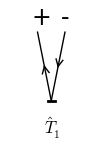
\includegraphics[width=46pt]{t1}
  \caption{}\label{fig:t1}
\endminipage\hfill
\minipage{.5\textwidth}
  \centering
  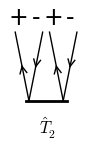
\includegraphics[width=44pt]{t2c}
  \caption{}\label{fig:t2}
\endminipage\hfill
\minipage{.5\textwidth}
  \centering
  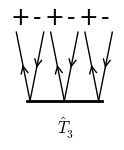
\includegraphics[width=60pt]{t3c}
  \caption{}\label{fig:t3}
\endminipage\hfill
\minipage{.5\textwidth}
  \centering
  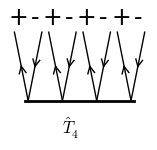
\includegraphics[width=80pt]{t4c}
  \caption{}\label{fig:t4}
\endminipage\hfill
\end{figure}



\subsection{Contractions of operators}

Analogous to Wicks's theorem, we need to find all possible ways to
contract the normal ordered Hamiltonian with strings of excitation
operators.  Our objective is thus to combine excitation operators,
possibly strings of excitation operators, with the various terms in
the normal ordered Hamiltonian, so they form topologically distinct
diagrams.

In Figs. \ref{fig:t1}, \ref{fig:t2}, \ref{fig:t3} and
\ref{fig:t4}, lines exiting the excitation operators are assigned a
number of plus and minus signs depending on the number of particle-
and hole lines in the operator. In the same way, we may assign plus or
minus signs to lines \emph{below} the interaction in the terms in the
normal ordered Hamiltonian. For strings of excitation operators, we
shall denote separations between the operators by a vertical line, so
that for example the product
\begin{equation}
\hat{T}_1 \hat{T}_2 \rightarrow + - \vert + - + - 
\label{eqn:exprod}
\end{equation}

Contractions will be represented diagrammatically as connecting
corresponding lines exiting the excitation operator and entering the
interaction vertex in the normal ordered Hamiltonian. The purpose of
the signs are to derive all topologically distinct connections between
these operators.

The plus and minus signs representing lines in the Hamiltonian term
must then \emph{all} connect to a corresponding sign in the string of
excitation operators, so that no lines entering or exiting below the
interaction is unconnected. At the same time, we seek only
combinations where at least one connection is made between the
Hamiltonian term and each of the excitation operators.

The practicalities of this procedure may be outlined in three steps.
First we must create any sequence containing the plus and minus signs
that occur in the Hamiltonian and the vertical bars from the string of
excitation operators. No vertical bars in this string of excitation
operators means that we have only one operator, and that no such
vertical bars should occur in the created sequence.

The next step is to consider all possible permutations of this
sequence. For each permutation we should first ensure that the diagram is \emph{linked} (see \ref{Chapter4}).

Contractions between the interaction and each of the excitation operators will be separated by
the vertical bars, so that unconnected operators may be identified by
either repeated vertical bars in the sequence as in
\begin{equation}
+ + \vert \vert - \vert -
\end{equation}
or by vertical bars at the start or end of the sequence as in

\begin{equation}
+ + \vert -\vert - \vert
\end{equation}



These connection patterns will correspond to unconnected diagrams and thus not contribute to the equations. 
Next, we need to ensure that the connection pattern is compatible to the operators, in the sense that the number
of connections of particle and holes ($+$ and $-$) to each excitation
operator must not exceed the corresponding plus and minus signs
present in the excitation operator.

\begin{figure}[hbtp]
 \centering
  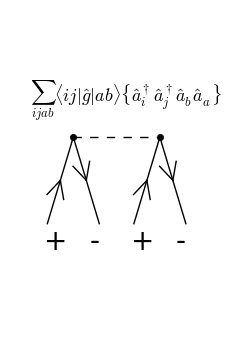
\includegraphics[width=120pt]{plusminus}
  \caption{Term in the normal ordered hamiltonian}\label{fig:plusminus}
\end{figure}

As an example, we may consider the Hamiltonian term in Fig.
\ref{fig:plusminus} connecting to the string of operators in Eq.
(\ref{eqn:exprod}). These will together produce the sequence
\begin{equation}
\hat{H_{N,9}} \hat{T}_1 \hat{T}_2 \rightarrow  + - + - \vert 
\end{equation}

Now, in the order above this is obviously not a contributing term or
even a possible connection pattern, since there are no connections
between $\hat{H}_N$ and $\hat{T}_2$, and the number of connections to
$\hat{T}_1$ exceeds the possible number of connections to this
operator.

However, considering the possible permutations of this sequence will
enable us to identify three distinct connection patterns which are
\begin{equation}
  + -\vert  + - \hspace{1cm}  -\vert  + + -  \hspace{1cm}  + \vert  + - -
\end{equation}

From these three connection patterns we may draw three different
diagrams, shown in Fig. \ref{fig:ht1t2}. These diagrams will in turn be
translated back into algebraic expressions that we work into our code.
\begin{figure}
 \centering
  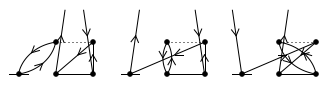
\includegraphics[width=320pt]{ht1t2}
  \caption{Diagrams produced by $\hat{H}_{N,9} \hat{T}_1 \hat{T}_2
    $. The diagrams are generated by our code and because of this the
    lines connect in a somewhat arbitrary fashion. Still, the diagrams
    are correct and non-ambiguous.}
\label{fig:ht1t2}
\end{figure}

A special case is when multiple occurrences of the same excitation
operators occur in the sequence. In this case the operators should be
treated as indistinguishable, so that only distinct connections occur.

For example we may consider the case of 

\begin{equation}
\hat{H_{N,9}} \hat{T}_2 \hat{T}_2 \rightarrow  + - + - \vert 
\end{equation}

The possible connection patterns from these operators are

\begin{equation}
  + -\vert  + - \hspace{1cm}  -\vert  + + -  \hspace{1cm}  + \vert  + - - \hspace{1cm}  ++ \vert  - -
\label{eqn:firstconnect}
\end{equation}

The last three terms could just as well be written

\begin{equation}
 + + -\vert  -  \hspace{1cm}  + - - \vert  + \hspace{1cm} - - \vert  + +
\end{equation}
but would not produce a diagram topologically distinct from the
connections in Eq. (\ref{eqn:firstconnect}), and is thereby excluded.


\subsection{Excitation level}

As may be seen from the diagrams in Fig. \ref{fig:ht1t2}, it is
fully possible for particles or holes in the excitation operator to
remain unconnected. In this case, we have three diagrams where all
have unconnected particle and hole lines. Such a diagram will produce
an excited Slater determinant, in this case creating a 1p1h (one
particle, one hole) state corresponding to the excitation level +1.

In other cases, we may have diagrams with no unconnected lines, corresponding to excitation level 0.

We will also have cases were particle and/or hole lines above the interaction cause excitations.

In general, we will find either zero or an even number of both particle- and hole lines unconnected in the diagram, and dividing the number of these by two will yield the excitation level.

The significance of the excitation level is that it quickly allows us to evaluate in which of the coupled cluster equations a diagram will contribute. Because of the orthonormality of the Slater determinants, only diagrams of excitation level 0 will contribute to the energy. Only diagrams of excitation level 2 will contribute to the t2-amplitude equation, and so on.

\subsection{Interpretation rules for diagrams}

Once all possible diagrams for a given sequence of operators are drawn, we will interpret them back into algebraic expressions that can be worked into code. The rules for interpreting diagrams are here just stated, pretty much as they appear in Shavitt and Bartlett's \emph{"Many Body Methods in Chemistry and Physics"} \cite[Chapter 9]{ShavittBartlett2009}.

\subsection{Label all lines}

Internal and external particle and hole lines are assigned labels. For
consistency and readability one should use the conventional naming
with letters \emph{"abcd..."} reserved for particles, and
\emph{"ijkl..."} for holes. Since the diagrams represents sum over
(internal) lines, it is preferable to reserve certain labels for
summation indices and other for "static" indices. This will be helpful
when writing the actual code.

\subsection{Identify the one-body operator}
Every one-body vertex should be interpreted as the one-body operator of the states exciting and entering the vertex, so that it produces an expression of the form $\hat{f}(p,q)$.

\subsection{Identify the two-body operator}
The two-body operator is identified as the two-body vertex with a dotted horizontal line, and the labels entering and/or leaving the vertex produce the following interaction:

\begin{equation}
\langle left out, right out \vert \vert left in, right in \rangle
\end{equation}

\subsection{Identify the amplitudes}
Each amplitude will occur as solid horizontal lines with particles and holes above it. Depending on the labeling, they are denoted algebraically as $\hat{t}^a_i$, $\hat{t}^{ab}_{ij}$, $\hat{t}^{abc}_{ijk}$ and $\hat{t}^{abcd}_{ijkl}$, for $\hat{T}_1$,$\hat{T}_2$,$\hat{T}_3$ and $\hat{T}_4$ respectively.

\subsection{Summation indices}
We then sum over all so-called internal indices that connect the
amplitudes to the interaction. These are easily identified as the only
connected lines in the diagram.

\subsection{Identify equivalent internal lines}
Equivalent lines are pairs of lines that connect at the same amplitude
and interaction, in the same direction (particle-particle or
hole-hole). For each such pair, we multiply the expression by a factor
of $\frac{1}{2}$.

\subsection{Identify equivalent \emph{T}-vertices}
$T$-vertices are considered equivalent if they connect to the same
interaction vertex in the same configurational pattern. For each such
pair, multiply by a factor of $\frac{1}{2}$.

\subsection{The phase factor}
Count the number of hole lines and loops, and multiply the expression
with a phase factor given by $(-)^{n_{holes}-n_{loops}}$. The number
of holes is the number of lines pointing downwards, and a loop is
easily identified as a pair of particle and hole lines connecting to
the same two vertices\footnote{Actually it is possible to draw
  diagrams in a manner that makes these loops hard to spot, but we
  shall not concern ourselves about this here.}.

\subsection{External permutations}
A pair of external lines (unconnected lines) are considered equivalent
if they connect to the same vertex. We must sum over all inequivalent
external lines, and include a parity factor of $(-)^{\sigma(P)}$ where
$\sigma(P)$ is the number of permutations.

\subsection{Cancel factors caused by external permutations}
For each pair of external lines connected to equivalent vertices, cancel one factor of $\frac{1}{2}$ caused by equivalent \emph{T}-vertices. 

\subsection{The correlation energy}
As may be seen from the energy equation (see Eq. (\ref{eqn:ccm1})), the diagrams that occur in this equation should have excitation level 0. When considering possible diagrams, this obviously means that the Hamiltonian term should not have any unconnected lines above the interaction, while all lines from the amplitudes should be connected to the interaction. In other words, we seek diagrams composed of only internal lines.

The only terms in the Hamiltonian that fulfill these criterions are the ones where all lines occur below the interaction, shown in Figs. \ref{fig:h1} and \ref{fig:h_9}. Considering the excitation level of these interactions, we find that they cause an excitation level of -1 for Fig. \ref{fig:h1} and -2 for Fig. \ref{fig:h_9}.

\begin{figure}[hbtp]
\minipage{.5\textwidth}
  \centering
  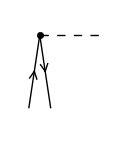
\includegraphics[width=46pt]{h1}
  \caption{}\label{fig:h1}
\endminipage\hfill
\minipage{.5\textwidth}
  \centering
  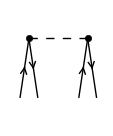
\includegraphics[width=44pt]{h_9}
  \caption{}\label{fig:h_9}
\endminipage\hfill
\end{figure}

It is then quite clear that only very few combinations are possible.
For example, no excitation beyond doubles will enter the energy
expression, since they will excite the reference state beyond the +2
level. Only the single excitation operator $\hat{T}_1$ (see
Fig. \ref{fig:t1}) will be able to produce an excitation level of +1,
and thus connect with the one-body operator in Fig. \ref{fig:h1}.

We will find a total of three different diagrams that contribute to
the energy, shown in Figs. \ref{fig:e1}, \ref{fig:e2} and
\ref{fig:e3}.

\begin{figure}[hbtp]
\minipage{.3\textwidth}
  \centering
  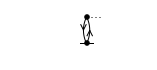
\includegraphics[width=100pt]{e1}
  \caption{}\label{fig:e1}
\endminipage\hfill
\minipage{.3\textwidth}
  \centering
  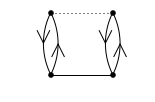
\includegraphics[width=80pt]{e2}
  \caption{}\label{fig:e2}
\endminipage\hfill
\minipage{.3\textwidth}
  \centering
  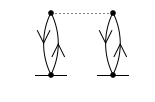
\includegraphics[width=80pt]{e3}
  \caption{}\label{fig:e3}
\endminipage\hfill
\end{figure}
 
To translate these diagrams into algebraic expressions, we apply the rules for diagram interpretation. We find 
\begin{equation}
\Delta e =  \sum_{ck} \langle k || c \rangle t_{k}^{c}+\frac{1}{4} \sum_{cdkl} \langle kl || cd \rangle t_{kl}^{cd}+\frac{1}{2} \sum_{ckdl} \langle kl || cd \rangle t_{k}^{c} t_{l}^{d}.
\label{eqn:c_energy}
\end{equation}

\section{Diagrams as code}

Although the diagrammatic rules greatly simplify the process of
deriving the equations, there is still a high probability for errors
due to human inaccuracy. The CCSD $\hat{T}_1$ amplitude equations have for example 14
terms, making even the diagrammatic process quite tedious. This is
reflected even in authoritative works on the subjects such as Shavitt
and Bartlett's \emph{"Many Body Methods in Chemistry and Physics"}
\cite{ShavittBartlett2009}, where errors in the equations have been
found\footnote{See as well Chapter 8 concerning the CCDT-1 validation.}.

Hermann Kümmel noted in his "Biography of the Coupled Cluster Method"
\cite{Kummel}, that

\emph{"Because of the often large number of terms in all versions of the CCM it is rather hard work to obtain the explicit equations by hand. And after this is done one has to write a program to put them into the computer."}

Is it really necessary to derive equations by hand and thereafter
write code manually? Probably not, and for this reason it makes sense
to ensure consistency in the derivation process by use of
computers. If equations are derived by the computer, we may also task
the computer to actually generate the code needed for numerical
computation.

A number of symbolic frameworks that can handle such operations
exists such as \emph{Second Quantization} for SymPy (Python)
\cite{secondquant}, but these are based on the algebraic approach with
Wick's theorem. As a part of the work on this thesis, a python script
was developed aimed at deriving the CC equations at any level of truncation
using the diagrammatic approach.

In this section, we shall briefly discuss how to translate the
diagrammatic rules into code, and then proceed to derive the explicit
equations for various truncations by use of this code.

\subsection{Implementation}

We will need to define operators in terms of unconnected lines above
and below the interaction. It is natural to define a class for these
operators, and define functions such as contractions that takes
operator classes as parameters. A function for contractions of
operators should return all distinct diagrams for the operators.

An operator is sufficiently described by its number of hole- and
particle lines above and below the vertex. This is easily translated
into two arrays for each operator, with a binary representation of
particle or holes (for example 0 and 1).

To perform contractions of such operators, we will first need to set
up the sequence of vertical bars and plus- and minus signs as
previously described. This is basically just a new array, created by
joining the array of particles and holes below the interaction vertex
with a number of vertical bars equal to the number of excitation
operators minus one.

The code then needs to seek through all possible permutations of this
sequence and identify the valid sequences. Such valid sequences may be
identified by connections between the Hamiltonian and all excitation
operators to its right, and by the number of connections occurring in
each excitation operator not exceeding the possible number of
connections.

Next we need to avoid over counting connection patterns due to
equivalent excitation operators, so we identify identical excitation
operators and keep only one of each such equivalent connection
pattern.

Finally we end up with a number of unique connection patterns that
gives us a non-ambiguous recipe for constructing the diagrams.

On top of this functionality we may want a framework for plotting the
diagrams or interpret them as algebraic expressions or code. IPython
Notebook \cite{ipython} provides an excellent environment for these
kinds of operations. In the following sections we will explore
such functionalities by discussing the software \emph{CCAlgebra} developed in connection with the work
with this thesis. The software \emph{CCAlgebra} allows one to derive automatically all possible approximations
in coupled cluster theory, providing thereby a benchmark to equations derived by paper and pencil. This provides an invaluable to benchmark the equations that enter our codes. Furthermore, the software \emph{CCAlgebra} allows also for automatic generation of code, as well as mathematical expressions and figures.

\subsection{CCAlgebra}

CCAlgebra is a python software developed by the present author  that may be imported into any IPython
notebook. It has no dependencies outside those libraries that are
normally included in extended python distributions such as Entougth
Canopy \cite{Entought} or Continuum Analytics Anaconda
\cite{Anaconda}.

To start a session one just starts IPython Notebook and imports the
CCAlgebra.py file into the notebook.
It is then possible to define operators in the following manner

\begin{minipage}{\linewidth}
\makebox[\linewidth]{
  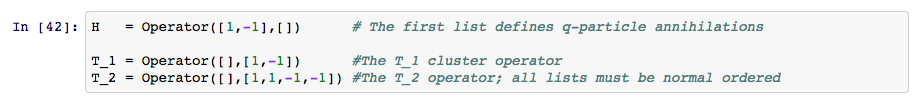
\includegraphics[keepaspectratio=true,scale=.5]{cca1}}  
\end{minipage}

Above we defined three operators; the Hamiltonian term from Fig.~\ref{fig:h1}, 
and the single and double excitation operators
$\hat{T}_1$ and $\hat{T}_2$. Each operator is fully described by two
lists; the first representing the pseudo particle annihilation
operators, while the second represents pseudo particle creation
operators.

To contract these operators we use a function that takes the
Hamiltonian operator and a list of excitation operators as parameters.

\begin{minipage}{\linewidth}
\makebox[\linewidth]{
  
\includegraphics[keepaspectratio=true,scale=.5]{cca2}}  
\end{minipage}

This will return an object that contains all possible diagrams
generated from the contraction of these operators. The reason for that
excitation operators should be brace-enclosed in a list is that this
list contains all excitation operators to the right of the
Hamiltonian, consistent with the prior derivation from the Hausdorff
expansion.

Some simple information may be obtained from the resulting
contraction, such as the excitation level and the number of resulting
distinct diagrams

\begin{minipage}{\linewidth}
\makebox[\linewidth]{
  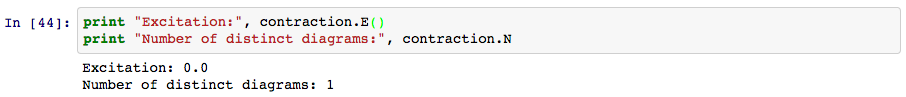
\includegraphics[keepaspectratio=true,scale=.5]{cca3}}  
\end{minipage}

The resulting diagrams are numbered from 0 and up, so as we only have
one diagram resulting from this contraction we may display it as latex
formatted text by the \emph{.latex()} method

\begin{minipage}{\linewidth}
\makebox[\linewidth]{
  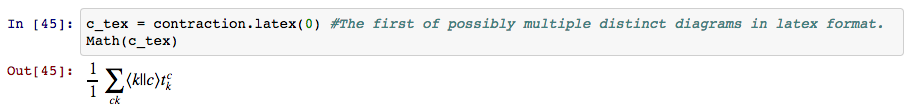
\includegraphics[keepaspectratio=true,scale=.5]{cca4}}  
\end{minipage}

We may also display it as a diagram by using the \emph{.diagram()} method.

\begin{minipage}{\linewidth}
\makebox[\linewidth]{
  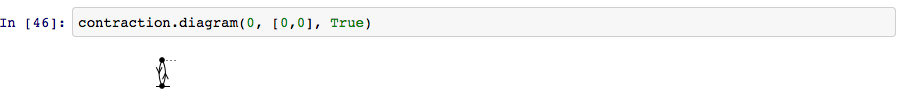
\includegraphics[keepaspectratio=true,scale=.5]{cca5}}  
\end{minipage}

The first parameter here specifies the number of the diagram
(beginning with 0), coordinates on the screen if we would like to
display multiple diagrams in the same frame, and finally an on/off
option for using built in formatting (turning of axis and scaling) or
letting the outside script adjust these parameters ("false").

With the computer's understanding of the diagram it is now very easy to translate it directly into code:

\begin{minipage}{\linewidth}
\makebox[\linewidth]{
  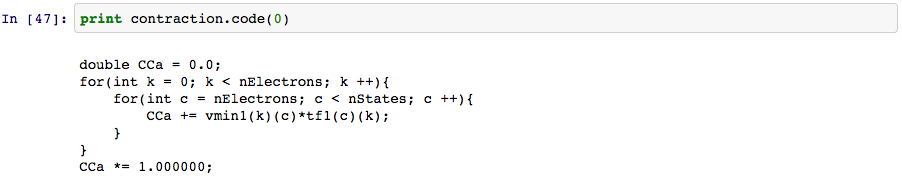
\includegraphics[keepaspectratio=true,scale=.5]{cca6}}  
\end{minipage}

In this case, the code is a naive C++ implementation (\emph{naive} in
the sense that it is the most direct translation of the diagram, using
for-loops where sums occur), but in principle it is possible to
generate any kind of code. Quite possibly also highly optimized code
if we supply the CCAlgebra script with some more information about the
system we want to calculate.

Terms in the CC equations may now be represented as code, diagrams or
mathematical expressions depending on how we prefer to view them. It does make sense to
refer to these terms simply as "diagrams".

We may of course now easily derive more complex diagrams, simply by defining the operators we seek:

\begin{minipage}{\linewidth}
\makebox[\linewidth]{
  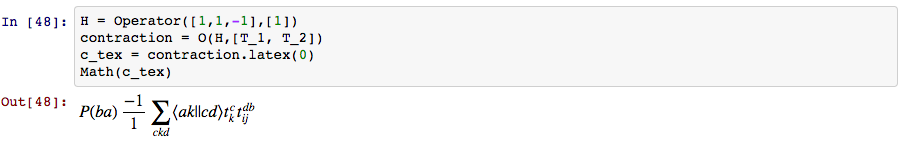
\includegraphics[keepaspectratio=true,scale=.5]{cca7}}  
\end{minipage}

Many physicists find diagrams helpful to quickly gain insight into the
nature of a given contribution. We have thus  added to our software 
the functionality to quickly render diagrams on screen.

\begin{minipage}{\linewidth}
\makebox[\linewidth]{
  \includegraphics[keepaspectratio=true,scale=.5]{cca8}}  
\end{minipage}

In this case we used a two-body term from the Hamiltonian, and we sum
over three internal lines. This results in a more computationally
intensive code with three nested for-loops:

\begin{minipage}{\linewidth}
\makebox[\linewidth]{
  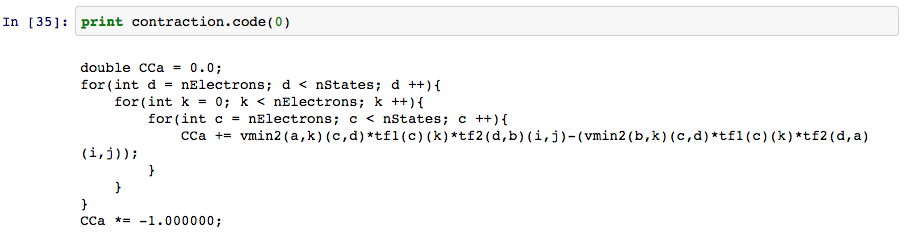
\includegraphics[keepaspectratio=true,scale=.5]{cca9}}  
\end{minipage}

In our equations the cluster operator occurs in a power series,
resulting in a multitude of products of excitation operators. To
handle this more easily and avoid the need to precalculate these, some
complementary functions to quickly evaluate such expanded power series
of the cluster operator is included:

\begin{minipage}{\linewidth}
\makebox[\linewidth]{
  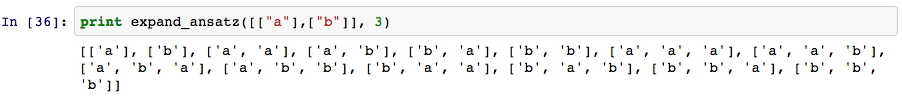
\includegraphics[keepaspectratio=true,scale=.5]{cca10}}  
\end{minipage}

It is also convenient to predefine some operators that occur often. A normal ordered Hamiltonian will come in handy:

\begin{minipage}{\linewidth}
\makebox[\linewidth]{
  \includegraphics[keepaspectratio=true,scale=.5]{cca11}}  
\end{minipage}

\subsection{Deriving amplitude equations using CCAlgebra}

Another convenient tool is a function that produces all possible
diagrams with a given excitation level from a normal ordered
Hamiltonian and the expanded exponential ansatz, in effect generating
the full energy- and amplitude equations. In the following example we
find all contributions to the $\hat{T}_1$ amplitude equation in the CCSD
truncation ($\hat{T} = \hat{T}_1 + \hat{T}_2$)

\begin{minipage}{\linewidth}
\makebox[\linewidth]{
  \includegraphics[keepaspectratio=true,scale=.5]{cca12}}  
\end{minipage}

The diagram are still a bit awkwardly formatted, but they are correct:

\begin{minipage}{\linewidth}
\makebox[\linewidth]{
  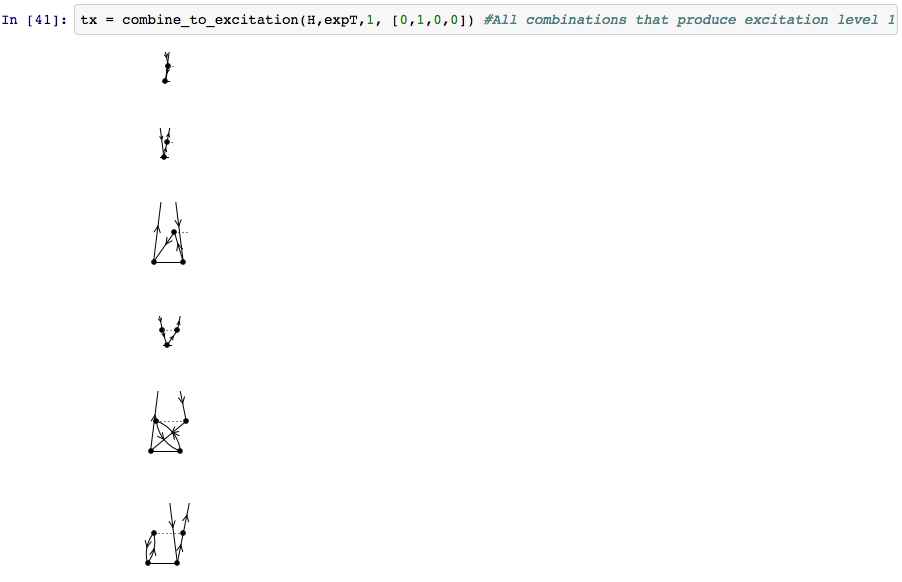
\includegraphics[keepaspectratio=true,scale=.5]{cca13}}  
\end{minipage}

\subsection{Deriving the energy using CCalgebra}

We have already noted how only a very few terms enter the energy
equations. Using CCAlgebra we may confirm that this is the indeed the
case

\begin{minipage}{\linewidth}
\makebox[\linewidth]{
  \includegraphics[keepaspectratio=true,scale=.5]{cca15}}  
\end{minipage}

By using CCAlgebra we may now go on to derive the explicit equations for the various CC methods. 

\subsection{Validation of CCAlgebra}

The developement of the CCAlgebra framework was mainly intended as an educational tool for better understanding of the CC equations and their derivation. As such, the code is written mainly as a proof of concept. 

Although the generated code from CCAlgebra is not optimized to such an
extent that it will be usable for the system we explore in this
thesis, it is fully capable to generate code that reproduces accurate
results for well-known systems such as CCSD dissociation energies for
the hydrogen molecule using a Gaussian basis set, as briefly described
in the section on size consistency. The code generated by CC algebra
was in exact agreement with the  code written by the present author for the CCSD case with
only minor manual edits in the C++ code.

To a certain extent this validates the results obtained by the use of
CCAlgebra, but it is still highly recommended to compare the equations
and diagrams with the ones present in the literature before
implementation.

\section{The CCD equations}

If we include only the double excitation operator in our cluster
operator we get the CCD (Coupled Cluster Doubles) equations. This
means that we let
\begin{equation}
\hat{T} = \hat{T}_2.
\end{equation}
We then perform the contractions with CCAlgebra. Since no single
excitations is included, we get an even simpler expression for the
energy than what we had earlier
\begin{equation}
\Delta e = \frac{1}{4} \sum_{cdkl} \langle kl || cd \rangle t_{kl}^{cd}.
\end{equation}

The only amplitude equation in this truncation is for $\hat{T}_2$:
\begin{multline}
0 =\langle ab \vert \vert ij \rangle + 
P(ij) \sum_{k} f_{kj} t_{ki}^{ab}+P(ab) \sum_{c} f_{bc} t_{ij}^{ac}+
\frac{1}{2} \sum_{cd} \langle ab \vert \vert cd \rangle t_{ij}^{cd} \\
+\frac{1}{2} \sum_{kl} \langle kl \vert \vert ij \rangle t_{kl}^{ab}-
P(ba)P(ij) \sum_{ck} \langle ak \vert \vert cj \rangle t_{ik}^{cb}- 
P(ij)\frac{1}{2} \sum_{cdkl} \langle kl \vert \vert cd \rangle t_{ik}^{cd} t_{jl}^{ab}\\
+\frac{1}{4} \sum_{cdkl} \langle kl \vert \vert cd \rangle t_{ij}^{cd} t_{kl}^{ab}-
 P(ab)\frac{1}{2} \sum_{ckld} \langle kl \vert \vert cd \rangle t_{kl}^{ca} t_{ij}^{db}+
P(ab)P(ij)\frac{1}{2} \sum_{ckdl} \langle kl \vert \vert cd \rangle t_{ik}^{ca} t_{jl}^{db}.
\end{multline}

There are a lot of different diagrams occurring in the CC
equations and it will make sense to classify them in ways that make
them more easily distinguishable. What is common to all diagrams is that
they contain only one Hamiltonian term contracted to possibly more
than one excitation operator. For this reason we may classify them
into orders of the various excitation operators occurring in them, and
in this simple case with only one excitation operator we may assign a
letter $L$ to diagrams \emph{linear} in $\hat{T}_2$ and the letter $Q$ to diagrams
\emph{quadratic} in $\hat{T}_2$. Since there are multiple diagrams
corresponding to each letter, we also assign a subscript letter in
their order of appearance.

The naming of each diagram is listed in table
\ref{tab:CCD_diagrams1}, but for now we just group together the terms
accordingly and define
\begin{multline}
L(t^{ab}_{ij}) \equiv 
\frac{1}{2} \sum_{cd} \langle ab \vert \vert cd \rangle t_{ij}^{cd} +
\frac{1}{2} \sum_{kl} \langle kl \vert \vert ij \rangle t_{kl}^{ab}-
P(ba)P(ij) \sum_{ck} \langle ak \vert \vert cj \rangle t_{ik}^{cb} .\\ 
\end{multline}
\begin{multline}
Q(t^{ab}_{ij}t^{ab}_{ij}) \equiv 
P(ij)\frac{1}{2} \sum_{cdkl} \langle kl \vert \vert cd \rangle t_{ik}^{cd} t_{jl}^{ab} 
+\frac{1}{4} \sum_{cdkl} \langle kl \vert \vert cd \rangle t_{ij}^{cd} t_{kl}^{ab} \\ - 
P(ab)\frac{1}{2} \sum_{ckld} \langle kl \vert \vert cd \rangle t_{kl}^{ca} t_{ij}^{db}+
P(ab)P(ij)\frac{1}{2} \sum_{ckdl} \langle kl \vert \vert cd \rangle t_{ik}^{ca} t_{jl}^{db},
\end{multline}
and write the CCD equation
\begin{equation}
0 =\langle ab \vert \vert ij \rangle + P(ij) \sum_{k} f_{kj} t_{ki}^{ab}+P(ab) \sum_{c} f_{bc} t_{ij}^{ac} + L(t^{ab}_{ij}) + Q(t^{ab}_{ij}t^{ab}_{ij}).
\end{equation}
It is not immediately clear how we are supposed to solve this
equation, but it is possible to rearrange the terms so that a
self-consistency criteria is found. This may be done by factoring out
the diagonal elements in the diagrams containing the one-body
operator, so that
\begin{equation}
P(ij) \sum_{k} f_{kj} t_{ki}^{ab} = \sum_{k \neq j} f_{kj} t_{ki}^{ab} + f_{jj} t_{ji}^{ab} - \sum_{k \neq i} f_{ki} t_{kj}^{ab}   - f_{ii} t_{ij}^{ab} =  -(f_{jj} + f_{ii}) t_{ij}^{ab} + \sum_{k \neq j} f_{kj} t_{ki}^{ab}  - \sum_{k \neq i} f_{ki} t_{kj}^{ab}  ,
\end{equation}
and
\begin{equation}
P(ab) \sum_{c} f_{ac} t_{ij}^{cb} = \sum_{c \neq a} f_{ac} t_{ij}^{cb} + f_{aa} t_{ij}^{ab} - \sum_{c \neq b} f_{bc} t_{ij}^{ca} -   f_{bb} t_{ij}^{ba} = (f_{aa} + f_{bb}) t_{ij}^{ab} +  \sum_{c \neq a} f_{ac} t_{ij}^{cb} - \sum_{c \neq b} f_{bc} t_{ij}^{ca}.
\end{equation}

In a canonical Hartree-Fock basis the one-body operator will only
contain diagonal elements, and since we will do all upcoming
calculations in such a basis we might as well ignore these non-diagonal sums. The full CCD amplitude equation then becomes
\begin{equation}
0 =\langle ab \vert \vert ij \rangle -(f_{jj} + f_{ii}) t_{ij}^{ab}+(f_{aa} + f_{bb}) t_{ij}^{ab}+L(t^{ab}_{ij}) + Q(t^{ab}_{ij}t^{ab}_{ij}).
\end{equation}
We may rewrite this expression to
\begin{equation}
 t_{ij}^{ab} =\frac{\langle ab \vert \vert ij \rangle+L(t^{ab}_{ij}) + Q(t^{ab}_{ij}t^{ab}_{ij})}{f_{jj} + f_{ii} - f_{aa} - f_{bb} }.
\end{equation}
With this expression we will be able to iteratively obtain self
consistence of the amplitudes. A reasonable guess for initial value
for the amplitudes is found by letting the $L$ and $Q$ term be zero,
so we have
\begin{equation}
 t_{ij}^{ab} =\frac{\langle ab \vert \vert ij \rangle}{f_{jj} + f_{ii} - f_{aa} - f_{bb} }.
\label{eqn:initialguess}
\end{equation}
These amplitudes actually correspond to second order in many-body perturbation energy, since
the evaluation of the energy expression for the CCD upon initialization yields
\begin{equation}
\Delta e^{(2)} =\frac{\langle ij \vert \vert ab \rangle \langle ab \vert \vert ij \rangle}{f_{jj} + f_{ii} - f_{aa} - f_{bb} }.
\label{eqn:initialenergy}
\end{equation}


\begin{table}[]
\centering
\caption{Diagrams CCD amplitude equation}
\label{tab:CCD_diagrams1}
\begin{tabular}{lllll}
Name & Factor & Permutation & Interpretation & Diagram \\
$$ & $-1$ & $P(ba)$ &$ \sum_{c} f_{a, c} t_{ij}^{cb}$  & 
\includegraphics[height=10mm]{CCD_0_3_0.png} \\  
$$ &  & $P(ij)$ &$ \sum_{k} f_{k, j} t_{ik}^{ab}$  & 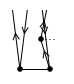
\includegraphics[height=10mm]{CCD_1_3_0.png} \\ 
$L_a$ & $\frac{1}{2}$ & &$ \sum_{cd} \langle ab \vert \vert cd \rangle t_{ij}^{cd}$  & 
\includegraphics[height=10mm]{CCD_4_3_0.png} \\  
$L_b$ & $\frac{1}{2}$ & &$ \sum_{kl} \langle kl \vert \vert ij \rangle t_{kl}^{ab}$  & 
\includegraphics[height=10mm]{CCD_5_3_0.png} \\ 
$L_c$ & $-1$ & $P(ba)P(ij)$ &$ \sum_{ck} \langle ak \vert \vert cj \rangle t_{ik}^{cb}$  & \includegraphics[height=10mm]{CCD_6_3_0.png} \\ 
$Q_a (D_{3a}) $ & $\frac{1}{4}$ & $$ &$ \sum_{cdkl} \langle kl \vert \vert cd \rangle t_{ij}^{cd} t_{kl}^{ab}$  & \includegraphics[height=10mm]{CCSD_t2_12_12_1.png} \\
$Q_b (D_{3b})  $ & $\frac{1}{2}$ & $P(ab)P(ij)$ &$ \sum_{ckdl} \langle kl \vert \vert cd \rangle t_{ik}^{ca} t_{jl}^{db}$  & \includegraphics[height=10mm]{CCSD_t2_12_12_3.png} \\
$Q_c (D_{3c}) $ & $-\frac{1}{2}$ & $P(ab)$ &$ \sum_{ckld} \langle kl \vert \vert cd \rangle t_{kl}^{ca} t_{ij}^{db}$  & \includegraphics[height=10mm]{CCSD_t2_12_12_2.png} \\
$Q_d (D_{3d}) $ & $-\frac{1}{2}$ & $P(ij)$ &$ \sum_{cdkl} \langle kl \vert \vert cd \rangle t_{ik}^{cd} t_{jl}^{ab}$  & \includegraphics[height=10mm]{CCSD_t2_12_12_0.png} \\
\end{tabular}
\end{table}

\FloatBarrier


\section{The CCSD equations}
To improve upon the results from the CCD truncation the next step is to include single excitations from the $\hat{T}_1$ excitation operator. Although no such excitations occur on the system subject to this thesis, we review this contributions here for completeness. 

By inclusion of the single excitations, we have the cluster operator
\begin{equation}
\hat{T} = \hat{T}_1 + \hat{T}_2.
\end{equation}
The diagrams contributing to the amplitude equations for $\hat{T}_1$
and $\hat{T}_2$ are given in tables \ref{tab:CCSD_t1_correct} and
\ref{tab:CCSD_t2_correct1} \ref{tab:CCSD_t2_correct1}.

In the same way as for the $\hat{T}_2$ amplitude, we may factor out terms from
diagrams $S_{3a}$ and $S_{3b}$ to initialize the $\hat{T}_1$ amplitude, resulting in
\begin{equation}
t_i^a = \frac{f_{a,i}}{f(i,i) - f(a,a)}  .
\end{equation}
The next amplitude is found in the same manner as for the $\hat{T}_2$ amplitude
for the CCD approximation, and we iterate until some convergence
criteria is fulfilled.

%Sign inconsistencies: S5a, D5a,  D6a, D6b

%Errors: S6 (occurred triply, treated t_1 as distinguishable)

%Not interpreted properly (interaction) D4a, D4b (manually corrected)

%check later: D8b

\begin{table}[]
\centering
\caption{Contributions to the CCSD $\hat{T}_1$ amplitude equation}
\label{tab:CCSD_t1_correct}
\begin{tabular}{lllll}
Name & Factor & Permutation & Interpretation & Diagram\\
$S_{3a}$ &  & $$ &$ \sum_{c} f_{a, c} t_{i}^{c}$  & \includegraphics[height=10mm]{CCSD_t1_1_9_0.png} \\
$S_{3b}$ & $-1$ & $$ &$ \sum_{k} f_{k, i} t_{k}^{a}$  & \includegraphics[height=10mm]{CCSD_t1_0_9_0.png} \\
$S_{5a}$ &  & $$ &$ \sum_{ck} f_{k, c} t_{i}^{c} t_{k}^{a}$  & \includegraphics[height=10mm]{CCSD_t1_3_5_0.png} \\
$S_{2a}$ &  & $$ &$ \sum_{ck} f_{k, c} t_{ik}^{ca}$  & \includegraphics[height=10mm]{CCSD_t1_3_13_0.png} \\
$S_{3c}$ & $-1$ & $$ &$ \sum_{ck} \langle ak \vert \vert ci \rangle t_{k}^{c}$  & \includegraphics[height=10mm]{CCSD_t1_6_9_0.png} \\
$S_{5b}$ &  & $$ &$ \sum_{ckd} \langle ak \vert \vert cd \rangle t_{k}^{c} t_{i}^{d}$  & \includegraphics[height=10mm]{CCSD_t1_10_5_0.png} \\
$S_{2b}$ & $\frac{1}{2}$ & $$ &$ \sum_{cdk} \langle ak \vert \vert cd \rangle t_{ik}^{cd}$  & \includegraphics[height=10mm]{CCSD_t1_10_13_0.png} \\
$S_{5c}$ & $-1$ & $$ &$ \sum_{ckl} \langle kl \vert \vert ci \rangle t_{k}^{c} t_{l}^{a}$  & \includegraphics[height=10mm]{CCSD_t1_8_5_0.png} \\
$S_{2c}$ & $-\frac{1}{2}$ & $$ &$ \sum_{ckl} \langle kl \vert \vert ci \rangle t_{kl}^{ca}$  & \includegraphics[height=10mm]{CCSD_t1_8_13_0.png} \\
$S_6$ &  & $$ &$ \sum_{ckdl} \langle kl \vert \vert cd \rangle t_{i}^{c} t_{k}^{a} t_{l}^{d}$  & \includegraphics[height=10mm]{CCSD_t1_12_2_1.png} \\
$S_{4c}$ &  & $$ &$ \sum_{ckdl} \langle kl \vert \vert cd \rangle t_{k}^{c} t_{il}^{da}$  & \includegraphics[height=10mm]{CCSD_t1_12_8_0.png} \\
$S_{4a}$ & $\frac{1}{2}$ & $$ &$ \sum_{cdkl} \langle kl \vert \vert cd \rangle t_{i}^{c} t_{kl}^{da}$  & \includegraphics[height=10mm]{CCSD_t1_12_8_2.png} \\
$S_{4b}$ & $\frac{1}{2}$ & $$ &$ \sum_{kcdl} \langle kl \vert \vert cd \rangle t_{k}^{a} t_{il}^{cd}$  & \includegraphics[height=10mm]{CCSD_t1_12_8_1.png} \\
\end{tabular}
\end{table}

\begin{table}[]
\centering
\caption{Contributions to the CCSD $\hat{T}_2$ amplitude equation (1)}
\label{tab:CCSD_t2_correct1}
\begin{tabular}{lllll}
Name & Factor & Permutation & Interpretation & Diagram\\
$$ & $-1$ & $P(ba)$ &$ \sum_{c} f_{a, c} t_{ij}^{cb}$  & \includegraphics[height=10mm]{CCD_1_3_0.png} \\  
$$ &  & $P(ij)$ &$ \sum_{k} f_{k, j} t_{ik}^{ab}$  & \includegraphics[height=10mm]{CCD_0_3_0.png} \\ 
$L_a$ & $\frac{1}{2}$ & &$ \sum_{cd} \langle ab \vert \vert cd \rangle t_{ij}^{cd}$  & \includegraphics[height=10mm]{CCD_5_3_0.png} \\  
$L_b$ & $\frac{1}{2}$ & &$ \sum_{kl} \langle kl \vert \vert ij \rangle t_{kl}^{ab}$  & \includegraphics[height=10mm]{CCD_4_3_0.png} \\ 
$L_c$ & $-1$ & $P(ba)P(ij)$ &$ \sum_{ck} \langle ak \vert \vert cj \rangle t_{ik}^{cb}$  & \includegraphics[height=10mm]{CCD_6_3_0.png} \\ 
$D_{3a} $ & $\frac{1}{4}$ & $$ &$ \sum_{cdkl} \langle kl \vert \vert cd \rangle t_{ij}^{cd} t_{kl}^{ab}$  & \includegraphics[height=10mm]{CCSD_t2_12_12_1.png} \\
$D_{3b}  $ & $\frac{1}{2}$ & $P(ab)P(ij)$ &$ \sum_{ckdl} \langle kl \vert \vert cd \rangle t_{ik}^{ca} t_{jl}^{db}$  & \includegraphics[height=10mm]{CCSD_t2_12_12_3.png} \\
$D_{3c} $ & $-\frac{1}{2}$ & $P(ab)$ &$ \sum_{ckld} \langle kl \vert \vert cd \rangle t_{kl}^{ca} t_{ij}^{db}$  & \includegraphics[height=10mm]{CCSD_t2_12_12_0.png} \\
$D_{3d} $ & $-\frac{1}{2}$ & $P(ij)$ &$ \sum_{cdkl} \langle kl \vert \vert cd \rangle t_{ik}^{cd} t_{jl}^{ab}$  & \includegraphics[height=10mm]{CCSD_t2_12_12_2.png} \\
$D_{5a}$ & $-1$ & $P(ij)$ &$ \sum_{ck} f_{k, c} t_{i}^{c} t_{jk}^{ab}$  & \includegraphics[height=10mm]{CCSD_t2_3_8_1.png} \\
$D_{5b}$ & $-1$ & $P(ab)$ &$ \sum_{kc} f_{k, c} t_{k}^{a} t_{ij}^{cb}$  & \includegraphics[height=10mm]{CCSD_t2_3_8_0.png} \\
$D_{6a}$ & $-\frac{1}{2}$ & $P(ij)$ &$ \sum_{cd} \langle ab \vert \vert cd \rangle t_{i}^{c} t_{j}^{d}$  & \includegraphics[height=10mm]{CCSD_t2_5_5_0.png} \\
$D_{6b}$ & $-\frac{1}{2}$ & $P(ab)$ &$ \sum_{kl} \langle kl \vert \vert ij \rangle t_{k}^{a} t_{l}^{b}$  & \includegraphics[height=10mm]{CCSD_t2_4_5_0.png} \\
$D_{6c}$ & $-1$ & $P(ij)P(ba)$ &$ \sum_{ck} \langle ak \vert \vert cj \rangle t_{i}^{c} t_{k}^{b}$  & \includegraphics[height=10mm]{CCSD_t2_6_5_0.png} \\
$D_{4a}$ &  & $P(ij)$ &$ \sum_{c}  \langle ab \vert \vert cj \rangle t_{i}^{c}$  & \includegraphics[height=10mm]{CCSD_t2_9_9_0.png} \\
$D_{8a}$ & $\frac{1}{2}$ & $P(ij)P(ba)$ &$ \sum_{cdk} \langle ak \vert \vert cd \rangle t_{i}^{c} t_{j}^{d} t_{k}^{b}$  & \includegraphics[height=10mm]{CCSD_t2_10_2_0.png} \\
$D_{8b}$ & $\frac{1}{2}$ & $P(ij)P(ba)$ &$ \sum_{cdk} \langle ak \vert \vert cd \rangle t_{i}^{c} t_{j}^{d} t_{k}^{b}$  & \includegraphics[height=10mm]{CCSD_t2_8_2_0.png} \\
$D_{5g}$ & $-1$ & $P(ba)$ &$ \sum_{ckd} \langle ak \vert \vert cd \rangle t_{k}^{c} t_{ij}^{db}$  & \includegraphics[height=10mm]{CCSD_t2_10_8_0.png} \\
$D_{5c}$ &  & $P(ij)P(ba)$ &$ \sum_{cdk} \langle ak \vert \vert cd \rangle t_{i}^{c} t_{jk}^{db}$  & \includegraphics[height=10mm]{CCSD_t2_10_8_2.png} \\
$D_{5e}$ & $-\frac{1}{2}$ & $P(ab)$ &$ \sum_{kcd} \langle kb \vert \vert cd \rangle t_{k}^{a} t_{ij}^{cd}$  & \includegraphics[height=10mm]{CCSD_t2_10_8_1.png} \\
$D_{4b}$ & $-1$ & $P(ab)$ &$ \sum_{k} \langle kb \vert \vert ij \rangle t_{k}^{a}$  & \includegraphics[height=10mm]{CCSD_t2_7_9_0.png} \\
\end{tabular}
\end{table}


\begin{table}[]
\centering
\caption{Contributions to the CCSD $\hat{T}_2$ amplitude equation (2)}
\label{tab:CCSD_t2_correct2}
\begin{tabular}{lllll}
Name & Factor & Permutation & Interpretation & Diagram\\
$D_{8b}$ & $-\frac{1}{2}$ & $P(ij)P(ab)$ &$ \sum_{ckl} \langle kl \vert \vert cj \rangle t_{i}^{c} t_{k}^{a} t_{l}^{b}$  & \includegraphics[height=10mm]{CCSD_t2_10_2_0.png} \\
$D_{5h}$ &  & $P(ji)$ &$ \sum_{ckl} \langle kl \vert \vert ci \rangle t_{k}^{c} t_{jl}^{ab}$  & \includegraphics[height=10mm]{CCSD_t2_8_8_0.png} \\
$D_{5f}$ & $\frac{1}{2}$ & $P(ij)$ &$ \sum_{ckl} \langle kl \vert \vert cj \rangle t_{i}^{c} t_{kl}^{ab}$  & \includegraphics[height=10mm]{CCSD_t2_8_8_2.png} \\
$D_{5d}$ & $-1$ & $P(ab)P(ji)$ &$ \sum_{kcl} \langle kl \vert \vert ic \rangle t_{k}^{a} t_{jl}^{cb}$  & \includegraphics[height=10mm]{CCSD_t2_8_8_1.png} \\
$D_9$ & $\frac{1}{4}$ & $P(ij)P(ab)$ &$ \sum_{cdkl} \langle kl \vert \vert cd \rangle t_{i}^{c} t_{j}^{d} t_{k}^{a} t_{l}^{b}$  & \includegraphics[height=10mm]{CCSD_t2_12_0_0.png} \\
$D_{7d}$ & $-1$ & $P(ij)$ &$ \sum_{ckdl} \langle kl \vert \vert cd \rangle t_{k}^{c} t_{i}^{d} t_{jl}^{ab}$  & \includegraphics[height=10mm]{CCSD_t2_12_4_1.png} \\
$D_{7e}$ & $-1$ & $P(ab)$ &$ \sum_{ckld} \langle kl \vert \vert cd \rangle t_{k}^{c} t_{l}^{a} t_{ij}^{db}$  & \includegraphics[height=10mm]{CCSD_t2_12_4_0.png} \\
$D_{7a}$ & $-\frac{1}{4}$ & $P(ij)$ &$ \sum_{cdkl} \langle kl \vert \vert cd \rangle t_{i}^{c} t_{j}^{d} t_{kl}^{ab}$  & \includegraphics[height=10mm]{CCSD_t2_12_4_4.png} \\
$D_{7c}$ &  & $P(ij)P(ab)$ &$ \sum_{ckdl} \langle kl \vert \vert cd \rangle t_{i}^{c} t_{k}^{a} t_{jl}^{db}$  & \includegraphics[height=10mm]{CCSD_t2_12_4_3.png} \\
$D_{7b} $ & $-\frac{1}{4}$ & $P(ab)$ &$ \sum_{klcd} \langle kl \vert \vert cd \rangle t_{k}^{a} t_{l}^{b} t_{ij}^{cd}$  & \includegraphics[height=10mm]{CCSD_t2_12_4_2.png} \\
\end{tabular}
\end{table}

\FloatBarrier

\section{The CCSDT equations}

In this section we present the full CCSDT equations as they are
generated by our software CCAlgebra for completeness. A thorough (and authorative)
derivation and treatment of these equations may be found in
\cite{ShavittBartlett2009}. It should be noted that inconsistencies
were found between these equations and the ones derived in
\cite{ShavittBartlett2009} concerning the signs in diagrams $T_{1a}$,
$T_{1b}$, and that the signs as they appear in table
\ref{tab:CCSDT_diagrams3_correct} produced results more in agreement
with expectations. While the signs in \cite{ShavittBartlett2009}
produced CCD(T) energies above the CCD energy, the ones from CCAlgebra
produced energies lower than the CCD results (for the three-dimensional homogeneous electron gas),
as one would expect for our system.

For the CCSDT equations, we have the cluster operator
\begin{equation}
\hat{T} = \hat{T}_1 + \hat{T}_2 + \hat{T}_3.
\end{equation}

In table \ref{tab:CCSDT_t1}, all contributions to the CCSDT $\hat{T}_1$ equation are listed, and we find only one extra diagram compared to the CCSD truncation ($S_7$). The solution procedure for this equation will be the same as for the CCSD and $\hat{T}_1$ amplitudes.

In the CCSDT $\hat{T}_2$ amplitude, we find six additional diagrams when
comparing to the CCSD $\hat{T}_2$ amplitudes. The additional diagrams are
listed in table \ref{tab:CCSDT_t2}. The solution procedure for this
equation shall also be the same as for the CCSD and CCD $\hat{T}_2$ amplitudes,
by factoring out terms and using a self consistency procedure.

All contributions to the $\hat{T}_3$ amplitudes are listed in tables
\ref{tab:CCSDT_diagrams3_correct1} -
\ref{tab:CCSDT_diagrams3_correct2}. Following a similar factorization
procedure as for the previous equations, we may factor out terms from
diagrams $T_{2a}$ and $T_{2b}$ so we find

\begin{equation}
\epsilon^{abc}_{ijk} t^{abc}_{ijk} = T_{1a} + T_{1b} + T_{2c} + ... + T_{10a},
\label{eqn:t3_factor}
\end{equation}
where we have defined
\begin{equation}
\epsilon^{abc}_{ijk} = f(i,i) + f(j,j) + f(k,k) - f(a,a) - f(b,b) - f(c,c).
\label{eqn:t3_factor}
\end{equation}

\subsection{Computational cost}

The computational cost of the full CCSDT equation scales as $n_h^3
n_p^5$ per iteration, where $n_p$ is the number of particle states and
$n_h$ is the number of hole states \cite[p.316]{ShavittBartlett2009}.
This, as well as the fact that such amplitudes actually have to be
stored using $n_h^3 n_p^3$ preferably double precision floats, makes
implementation of the full CCSDT a formidable challenge.
 

\begin{table}[]
\centering
\caption{Contributions to the CCSDT $\hat{T}_1$ amplitude equation}
\label{tab:CCSDT_t1}
\begin{tabular}{lllll}
$S_{3a}$ &  & $$ &$ \sum_{c} f_{a, c} t_{i}^{c}$  & \includegraphics[height=10mm]{CCSD_t1_1_9_0.png} \\
$S_{3b}$ & $-1$ & $$ &$ \sum_{k} f_{k, i} t_{k}^{a}$  & \includegraphics[height=10mm]{CCSD_t1_0_9_0.png} \\
$S_{5a}$ &  & $$ &$ \sum_{ck} f_{k, c} t_{i}^{c} t_{k}^{a}$  & \includegraphics[height=10mm]{CCSD_t1_3_5_0.png} \\
$S_{2a}$ &  & $$ &$ \sum_{ck} f_{k, c} t_{ik}^{ca}$  & \includegraphics[height=10mm]{CCSD_t1_3_13_0.png} \\
$S_{3c}$ & $-1$ & $$ &$ \sum_{ck} \langle ak \vert \vert ci \rangle t_{k}^{c}$  & \includegraphics[height=10mm]{CCSD_t1_6_9_0.png} \\
$S_{5b}$ &  & $$ &$ \sum_{ckd} \langle ak \vert \vert cd \rangle t_{k}^{c} t_{i}^{d}$  & \includegraphics[height=10mm]{CCSD_t1_10_5_0.png} \\
$S_{2b}$ & $\frac{1}{2}$ & $$ &$ \sum_{cdk} \langle ak \vert \vert cd \rangle t_{ik}^{cd}$  & \includegraphics[height=10mm]{CCSD_t1_10_13_0.png} \\
$S_{5c}$ & $-1$ & $$ &$ \sum_{ckl} \langle kl \vert \vert ci \rangle t_{k}^{c} t_{l}^{a}$  & \includegraphics[height=10mm]{CCSD_t1_8_5_0.png} \\
$S_{2c}$ & $-\frac{1}{2}$ & $$ &$ \sum_{ckl} \langle kl \vert \vert ci \rangle t_{kl}^{ca}$  & \includegraphics[height=10mm]{CCSD_t1_8_13_0.png} \\
$S_6$ &  & $$ &$ \sum_{ckdl} \langle kl \vert \vert cd \rangle t_{i}^{c} t_{k}^{a} t_{l}^{d}$  & \includegraphics[height=10mm]{CCSD_t1_12_2_1.png} \\
$S_{4c}$ &  & $$ &$ \sum_{ckdl} \langle kl \vert \vert cd \rangle t_{k}^{c} t_{il}^{da}$  & \includegraphics[height=10mm]{CCSD_t1_12_8_0.png} \\
$S_{4a}$ & $\frac{1}{2}$ & $$ &$ \sum_{cdkl} \langle kl \vert \vert cd \rangle t_{i}^{c} t_{kl}^{da}$  & \includegraphics[height=10mm]{CCSD_t1_12_8_2.png} \\
$S_{4b}$ & $\frac{1}{2}$ & $$ &$ \sum_{kcdl} \langle kl \vert \vert cd \rangle t_{k}^{a} t_{il}^{cd}$  & \includegraphics[height=10mm]{CCSD_t1_12_8_1.png} \\
$S_7$ & $\frac{1}{4}$ & $$ &$ \sum_{cdkl} \langle kl \vert \vert cd \rangle t_{ikl}^{cda}$  & \includegraphics[height=10mm]{CCSDT_t1_12_33_0.png} \\
\end{tabular}
\end{table}


\begin{table}[]
\centering
\caption{Additional diagrams in the CCSDT $\hat{T}_2$ amplitude equation (1)}
\label{tab:CCSDT_t2}
\begin{tabular}{lllll}
Name & Factor & Permutation & Interpretation & Diagram\\
$D_{10a}$ &  & $$ &$ \sum_{ck} f_{k, c} t_{ijk}^{cab}$  & \includegraphics[height=10mm]{CCSD_t2_3_33_0.png} \\
$D_{10b}$ & $-\frac{1}{2}$ & $P(ba)$ &$ \sum_{cdk} \langle ak \vert \vert cd \rangle t_{ijk}^{cdb}$  & \includegraphics[height=10mm]{CCSD_t2_10_33_0.png} \\
$D_{10c}$ & $\frac{1}{2}$ & $P(ij)$ &$ \sum_{ckl} \langle kl \vert \vert cj \rangle t_{ikl}^{cab}$  & \includegraphics[height=10mm]{CCSD_t2_8_33_0.png} \\
$D_{11a}$ &  & $$ &$ \sum_{ckdl} \langle kl \vert \vert cd \rangle t_{k}^{c} t_{ijl}^{dab}$  & \includegraphics[height=10mm]{CCSD_t2_12_18_0.png} \\
$D_{11c}$ & $-\frac{1}{2}$ & $P(ij)$ &$ \sum_{cdkl} \langle kl \vert \vert cd \rangle t_{i}^{c} t_{jkl}^{dab}$  & \includegraphics[height=10mm]{CCSD_t2_12_18_2.png} \\
$D_{11b}$ & $-\frac{1}{2}$ & $P(ab)$ &$ \sum_{kcdl} \langle kl \vert \vert cd \rangle t_{k}^{a} t_{ijl}^{cdb}$  & \includegraphics[height=10mm]{CCSD_t2_12_18_1.png} \\
\end{tabular}
\end{table}


\begin{table}[]
\centering
\caption{Contributions to the CCSDT $\hat{T}_3$ amplitude equation (1)}
\label{tab:CCSDT_diagrams3_correct1}
\begin{tabular}{lllll}
Name & Factor & Permutation & Interpretation & Diagram\\
$T_{1a}$ & $-1$ & $P(ba)P(bz)P(iw)P(jw)$ &$ \sum_{c} \langle ab \vert \vert ck \rangle t_{ij}^{cb}$  & \includegraphics[height=10mm]{CC9_29_0.png} \\
$T_{1b}$ &  & $P(az)P(bz)P(ij)P(iw)$ &$ \sum_{k} \langle kz \vert \vert j \rangle t_{ik}^{ab}$  & \includegraphics[height=10mm]{CC7_29_0.png} \\
$T_{2a}$ &  & $P(ba)P(za)$ &$ \sum_{c} f_{a, c} t_{ijw}^{cbz}$  & \includegraphics[height=10mm]{CC1_33_0.png} \\
$T_{2b}$ & $-1$ & $P(iw)P(jw)$ &$ \sum_{k} f_{k, w} t_{ijk}^{abz}$  & \includegraphics[height=10mm]{CC0_33_0.png} \\
$T_{6a}$ &  & $P(ij)P(iw)$ &$ \sum_{ck} f_{k, c} t_{i}^{c} t_{jwk}^{abz}$  & \includegraphics[height=10mm]{CC3_18_1.png} \\
$T_{6b}$ &  & $P(ab)P(az)$ &$ \sum_{kc} f_{k, c} t_{k}^{a} t_{ijw}^{cbz}$  & \includegraphics[height=10mm]{CC3_18_0.png} \\
$T_{2c}$ & $\frac{1}{2}$ & $P(za)P(zb)$ &$ \sum_{cd} \langle ab \vert \vert cd \rangle t_{ijw}^{cdz}$  & \includegraphics[height=10mm]{CC5_33_0.png} \\
$T_{2d}$ & $\frac{1}{2}$ & $P(iw)P(ij)$ &$ \sum_{kl} \langle kl \vert \vert jw \rangle t_{ikl}^{abz}$  & \includegraphics[height=10mm]{CC4_33_0.png} \\
$T_{2e}$ & $-1$ & $P(ba)P(za)P(iw)P(jw)$ &$ \sum_{ck} \langle ak \vert \vert cw \rangle t_{ijk}^{cbz}$  & \includegraphics[height=10mm]{CC6_33_0.png} \\
$T_{3a}$ &  & $P(ab)P(az)P(iw)P(jw)$ &$ \sum_{ck} f_{k, c} t_{ij}^{ca} t_{wk}^{bz}$  & \includegraphics[height=10mm]{CC3_25_0.png} \\
$T_{3d}$ & $\frac{1}{2}$ & $P(iw)P(jw)P(ba)P(za)$ &$ \sum_{cdk} \langle ak \vert \vert cd \rangle t_{ij}^{cd} t_{wk}^{bz}$  & \includegraphics[height=10mm]{CC10_25_1.png} \\
$T_{3b}$ & $-1$ & $P(bz)P(ba)P(ij)P(iw)P(za)$ &$ \sum_{ckd} \langle ak \vert \vert cd \rangle t_{ik}^{cb} t_{jw}^{dz}$  & \includegraphics[height=10mm]{CC8_25_1.png} \\
$T_{3c}$ &  & $P(ab)P(az)P(iw)P(ij)P(wj)$ &$ \sum_{ckl} \langle kl \vert \vert cj \rangle t_{ik}^{ca} t_{wl}^{bz}$  & \includegraphics[height=10mm]{CC10_25_0.png} \\
$T_{3e}$ & $-\frac{1}{2}$ & $P(ab)P(az)P(iw)P(jw)$ &$ \sum_{ckl} \langle kl \vert \vert cw \rangle t_{ij}^{ca} t_{kl}^{bz}$  & \includegraphics[height=10mm]{CC8_25_0.png} \\
$T_{4a}$ &  & $P(ij)P(iw)P(za)P(zb)$ &$ \sum_{cd} \langle ab \vert \vert cd \rangle t_{i}^{c} t_{jw}^{dz}$  & \includegraphics[height=10mm]{CC5_15_0.png} \\
$T_{4b}$ &  & $P(ab)P(az)P(ji)P(jw)$ &$ \sum_{kl} \langle kl \vert \vert iw \rangle t_{k}^{a} t_{jl}^{bz}$  & \includegraphics[height=10mm]{CC4_15_0.png} \\
$T_{4c}$ &  & $P(ij)P(iw)P(ba)P(za)P(jw)$ &$ \sum_{ck} \langle ak \vert \vert cw \rangle t_{i}^{c} t_{jk}^{bz}$  & \includegraphics[height=10mm]{CC6_15_1.png} \\
$T_{4d}$ &  & $P(az)P(ab)P(zb)P(ji)P(wi)$ &$ \sum_{kc} \langle kb \vert \vert ic \rangle t_{k}^{a} t_{jw}^{cz}$  & \includegraphics[height=10mm]{CC6_15_0.png} \\
\end{tabular}
\end{table}

\begin{table}[]
\centering
\caption{Contributions to the CCSDT $\hat{T}_3$ amplitude equation (2)}
\label{tab:CCSDT_diagrams3_correct2}
\begin{tabular}{lllll}
$T_{6e}$ &  & $P(ba)P(za)$ &$ \sum_{ckd} \langle ak \vert \vert cd \rangle t_{k}^{c} t_{ijw}^{dbz}$  & \includegraphics[height=10mm]{CC10_18_0.png} \\
$T_{6c}$ &  & $P(ij)P(iw)P(ba)P(za)$ &$ \sum_{cdk} \langle ak \vert \vert cd \rangle t_{i}^{c} t_{jwk}^{dbz}$  & \includegraphics[height=10mm]{CC10_18_2.png} \\
$T_{6g}$ & $-\frac{1}{2}$ & $P(az)P(ab)P(zb)$ &$ \sum_{kcd} \langle kb \vert \vert cd \rangle t_{k}^{a} t_{ijw}^{cdz}$  & \includegraphics[height=10mm]{CC10_18_1.png} \\
$T_{6f}$ & $-1$ & $P(ji)P(wi)$ &$ \sum_{ckl} \langle kl \vert \vert ci \rangle t_{k}^{c} t_{jwl}^{abz}$  & \includegraphics[height=10mm]{CC8_18_0.png} \\
$T_{6h}$ & $\frac{1}{2}$ & $P(ij)P(iw)P(jw)$ &$ \sum_{ckl} \langle kl \vert \vert cw \rangle t_{i}^{c} t_{jkl}^{abz}$  & \includegraphics[height=10mm]{CC8_18_2.png} \\
$T_{6d}$ & $-1$ & $P(ab)P(az)P(ji)P(wi)$ &$ \sum_{kcl} \langle kl \vert \vert ic \rangle t_{k}^{a} t_{jwl}^{cbz}$  & \includegraphics[height=10mm]{CC8_18_1.png} \\
$T_{5b}$ & $\frac{1}{2}$ & $P(ij)P(iw)$ &$ \sum_{cdkl} \langle kl \vert \vert cd \rangle t_{ik}^{cd} t_{jwl}^{abz}$  & \includegraphics[height=10mm]{CC12_28_2.png} \\
$T_{5f}$ & $\frac{1}{4}$ & $P(iw)P(jw)$ &$ \sum_{cdkl} \langle kl \vert \vert cd \rangle t_{ij}^{cd} t_{wkl}^{abz}$  & \includegraphics[height=10mm]{CC12_28_5.png} \\
$T_{5c}$ & $\frac{1}{2}$ & $P(ab)P(az)$ &$ \sum_{ckld} \langle kl \vert \vert cd \rangle t_{kl}^{ca} t_{ijw}^{dbz}$  & \includegraphics[height=10mm]{CC12_28_0.png} \\
$T_{5a}$ &  & $P(ab)P(az)P(ij)P(iw)$ &$ \sum_{ckdl} \langle kl \vert \vert cd \rangle t_{ik}^{ca} t_{jwl}^{dbz}$  & \includegraphics[height=10mm]{CC12_28_3.png} \\
$T_{5d}$ & $\frac{1}{2}$ & $P(ab)P(az)P(iw)P(jw)$ &$ \sum_{cdkl} \langle kl \vert \vert cd \rangle t_{ij}^{ca} t_{wkl}^{dbz}$  & \includegraphics[height=10mm]{CC12_28_4.png} \\
$T_{5g}$ & $\frac{1}{4}$ & $P(az)P(bz)$ &$ \sum_{klcd} \langle kl \vert \vert cd \rangle t_{kl}^{ab} t_{ijw}^{cdz}$  & \includegraphics[height=10mm]{CC12_28_6.png} \\
$T_{5e}$ & $\frac{1}{2}$ & $P(az)P(bz)P(ij)P(iw)$ &$ \sum_{kcdl} \langle kl \vert \vert cd \rangle t_{ik}^{ab} t_{jwl}^{cdz}$  & \includegraphics[height=10mm]{CC12_28_1.png} \\
$T_{7c}$ & $-\frac{1}{2}$ & $P(ij)P(iw)P(jw)P(ba)P(za)$ &$ \sum_{cdk} \langle ak \vert \vert cd \rangle t_{i}^{c} t_{j}^{d} t_{wk}^{bz}$  & \includegraphics[height=10mm]{CC10_6_1.png} \\
$T_{7a}$ & $-1$ & $P(ij)P(iw)P(bz)P(ba)P(za)$ &$ \sum_{ckd} \langle ak \vert \vert cd \rangle t_{i}^{c} t_{k}^{b} t_{jw}^{dz}$  & \includegraphics[height=10mm]{CC10_6_0.png} \\
$T_{7b}$ &  & $P(iw)P(ij)P(ab)P(az)P(wj)$ &$ \sum_{ckl} \langle kl \vert \vert cj \rangle t_{i}^{c} t_{k}^{a} t_{wl}^{bz}$  & \includegraphics[height=10mm]{CC8_6_1.png} \\
$T_{7d}$ & $\frac{1}{2}$ & $P(ab)P(az)P(bz)P(ji)P(wi)$ &$ \sum_{klc} \langle kl \vert \vert ic \rangle t_{k}^{a} t_{l}^{b} t_{jw}^{cz}$  & \includegraphics[height=10mm]{CC8_6_0.png} \\
$T_{10b}$ & $-\frac{1}{2}$ & $P(ij)P(iw)P(jw)P(ab)P(az)$ &$ \sum_{cdkl} \langle kl \vert \vert cd \rangle t_{i}^{c} t_{j}^{d} t_{k}^{a} t_{wl}^{bz}$  & \includegraphics[height=10mm]{CC12_1_0.png} \\
$T_{10a}$ & $-\frac{1}{2}$ & $P(ij)P(iw)P(ab)P(az)P(bz)$ &$ \sum_{ckld} \langle kl \vert \vert cd \rangle t_{i}^{c} t_{k}^{a} t_{l}^{b} t_{jw}^{dz}$  & \includegraphics[height=10mm]{CC12_1_1.png} \\
\end{tabular}
\end{table}

\begin{table}[]
\centering
\caption{Contributions to the CCSDT $\hat{T}_3$ amplitude equation (3)}
\label{tab:CCSDT_diagrams3_correct}
\begin{tabular}{lllll}
$T_{9a}$ &  & $P(ij)P(iw)$ &$ \sum_{ckdl} \langle kl \vert \vert cd \rangle t_{k}^{c} t_{i}^{d} t_{jwl}^{abz}$  & \includegraphics[height=10mm]{CC12_8_1.png} \\
$T_{9b}$ &  & $P(ab)P(az)$ &$ \sum_{ckld} \langle kl \vert \vert cd \rangle t_{k}^{c} t_{l}^{a} t_{ijw}^{dbz}$  & \includegraphics[height=10mm]{CC12_8_0.png} \\
$T_{9c}$ & $-\frac{1}{4}$ & $P(ij)P(iw)P(jw)$ &$ \sum_{cdkl} \langle kl \vert \vert cd \rangle t_{i}^{c} t_{j}^{d} t_{wkl}^{abz}$  & \includegraphics[height=10mm]{CC12_8_4.png} \\
$T_{9e}$ &  & $P(ij)P(iw)P(ab)P(az)$ &$ \sum_{ckdl} \langle kl \vert \vert cd \rangle t_{i}^{c} t_{k}^{a} t_{jwl}^{dbz}$  & \includegraphics[height=10mm]{CC12_8_3.png} \\
$T_{9d}$ & $-\frac{1}{4}$ & $P(ab)P(az)P(bz)$ &$ \sum_{klcd} \langle kl \vert \vert cd \rangle t_{k}^{a} t_{l}^{b} t_{ijw}^{cdz}$  & \includegraphics[height=10mm]{CC12_8_2.png} \\
$T_{8a}$ &  & $P(ab)P(az)P(iw)P(jw)$ &$ \sum_{ckdl} \langle kl \vert \vert cd \rangle t_{k}^{c} t_{ij}^{da} t_{wl}^{bz}$  & \includegraphics[height=10mm]{CC12_12_0.png} \\
$T_{8b}$ & $-1$ & $P(ij)P(iw)P(ab)P(az)P(jw)$ &$ \sum_{cdkl} \langle kl \vert \vert cd \rangle t_{i}^{c} t_{jk}^{da} t_{wl}^{bz}$  & \includegraphics[height=10mm]{CC12_12_4.png} \\
$T_{8d}$ & $\frac{1}{2}$ & $P(ij)P(iw)P(ab)P(az)$ &$ \sum_{cdkl} \langle kl \vert \vert cd \rangle t_{i}^{c} t_{jw}^{da} t_{kl}^{bz}$  & \includegraphics[height=10mm]{CC12_12_3.png} \\
$T_{8e}$ & $\frac{1}{2}$ & $P(ab)P(az)P(iw)P(jw)$ &$ \sum_{kcdl} \langle kl \vert \vert cd \rangle t_{k}^{a} t_{ij}^{cd} t_{wl}^{bz}$  & \includegraphics[height=10mm]{CC12_12_2.png} \\
$T_{8c}$ & $-1$ & $P(ab)P(az)P(bz)P(ij)P(iw)$ &$ \sum_{kcld} \langle kl \vert \vert cd \rangle t_{k}^{a} t_{il}^{cb} t_{jw}^{dz}$  & \includegraphics[height=10mm]{CC12_12_1.png} \\
\end{tabular}
\end{table}


\FloatBarrier


\section{The CCDT equations}

The main aim of this thesis is to explore triple contributions in
coupled cluster theory for the homogeneous electron gas. For homogeneous
matter such as the electron gas, the singles contribution vanish due
to symmetry and momentum conservation \cite{Baardsen2014, Day1967}. For
this reason we will only need to include diagrams from the CCDT
(doubles - triples) truncation.
Furthermore, esome of the diagrams in the CCDT equations will
vanish due to the fact that we employ a canonical Hartree-Fock basis
\cite[p.314]{ShavittBartlett2009}. We may therefore omit the term
$D_{10a}$ from the $\hat{T}_2$ amplitude equation, and all diagrams containing
single excitations are omitted from the $\hat{T}_3$ amplitude equation (as
compared to the full CCSDT $\hat{T}_3$ equation.)


\begin{table}[]
\centering
\caption{Contributions to the CCDT $\hat{T}_2$ amplitude equation.}
\label{tab:CCDT_t2}
\begin{tabular}{lllll}
Name & Factor & Permutation & Interpretation & Diagram\\
$$ & $-1$ & $P(ba)$ &$ \sum_{c} f_{a, c} t_{ij}^{cb}$  & \includegraphics[height=10mm]{CCD_0_3_0.png} \\  
$$ &  & $P(ij)$ &$ \sum_{k} f_{k, j} t_{ik}^{ab}$  & \includegraphics[height=10mm]{CCD_1_3_0.png} \\ 
$L_a$ & $\frac{1}{2}$ & &$ \sum_{cd} \langle ab \vert \vert cd \rangle t_{ij}^{cd}$  & \includegraphics[height=10mm]{CCD_4_3_0.png} \\  
$L_b$ & $\frac{1}{2}$ & &$ \sum_{kl} \langle kl \vert \vert ij \rangle t_{kl}^{ab}$  & \includegraphics[height=10mm]{CCD_5_3_0.png} \\ 
$L_c$ & $-1$ & $P(ba)P(ij)$ &$ \sum_{ck} \langle ak \vert \vert cj \rangle t_{ik}^{cb}$  & \includegraphics[height=10mm]{CCD_6_3_0.png} \\ 
$D_{3a} $ & $\frac{1}{4}$ & $$ &$ \sum_{cdkl} \langle kl \vert \vert cd \rangle t_{ij}^{cd} t_{kl}^{ab}$  & \includegraphics[height=10mm]{CCSD_t2_12_12_1.png} \\
$D_{3b}  $ & $\frac{1}{2}$ & $P(ab)P(ij)$ &$ \sum_{ckdl} \langle kl \vert \vert cd \rangle t_{ik}^{ca} t_{jl}^{db}$  & \includegraphics[height=10mm]{CCSD_t2_12_12_3.png} \\
$D_{3c} $ & $-\frac{1}{2}$ & $P(ab)$ &$ \sum_{ckld} \langle kl \vert \vert cd \rangle t_{kl}^{ca} t_{ij}^{db}$  & \includegraphics[height=10mm]{CCSD_t2_12_12_2.png} \\
$D_{3d} $ & $-\frac{1}{2}$ & $P(ij)$ &$ \sum_{cdkl} \langle kl \vert \vert cd \rangle t_{ik}^{cd} t_{jl}^{ab}$  & \includegraphics[height=10mm]{CCSD_t2_12_12_0.png} \\
$D_{10b}$ & $-\frac{1}{2}$ & $P(ba)$ &$ \sum_{cdk} \langle ak \vert \vert cd \rangle t_{ijk}^{cdb}$  & \includegraphics[height=10mm]{CCSD_t2_10_33_0.png} \\
$D_{10c}$ & $\frac{1}{2}$ & $P(ij)$ &$ \sum_{ckl} \langle kl \vert \vert cj \rangle t_{ikl}^{cab}$  & \includegraphics[height=10mm]{CCSD_t2_8_33_0.png} \\
\end{tabular}
\end{table}

\begin{table}[]
\centering
\caption{Contributions to the CCDT $\hat{T}_3$ amplitude equation.}
\label{tab:CCDT_t3}
\begin{tabular}{lllll}
Name & Factor & Permutation & Interpretation & Diagram\\
$T_{1a}$ & $-1$ & $P(ba)P(bz)P(iw)P(jw)$ &$ \sum_{c} \langle ab \vert \vert ck \rangle t_{ij}^{cb}$  & \includegraphics[height=10mm]{CC9_29_0.png} \\
$T_{1b}$ &  & $P(az)P(bz)P(ij)P(iw)$ &$ \sum_{k} \langle kz \vert \vert j \rangle t_{ik}^{ab}$  & \includegraphics[height=10mm]{CC7_29_0.png} \\
$T_{2a}$ &  & $P(ba)P(za)$ &$ \sum_{c} f_{a, c} t_{ijw}^{cbz}$  & \includegraphics[height=10mm]{CC1_33_0.png} \\
$T_{2b}$ & $-1$ & $P(iw)P(jw)$ &$ \sum_{k} f_{k, w} t_{ijk}^{abz}$  & \includegraphics[height=10mm]{CC0_33_0.png} \\
$T_{2c}$ & $\frac{1}{2}$ & $P(za)P(zb)$ &$ \sum_{cd} \langle ab \vert \vert cd \rangle t_{ijw}^{cdz}$  & \includegraphics[height=10mm]{CC5_33_0.png} \\
$T_{2d}$ & $\frac{1}{2}$ & $P(iw)P(ij)$ &$ \sum_{kl} \langle kl \vert \vert jw \rangle t_{ikl}^{abz}$  & \includegraphics[height=10mm]{CC4_33_0.png} \\
$T_{2e}$ & $-1$ & $P(ba)P(za)P(iw)P(jw)$ &$ \sum_{ck} \langle ak \vert \vert cw \rangle t_{ijk}^{cbz}$  & \includegraphics[height=10mm]{CC6_33_0.png} \\
$T_{3d}$ & $\frac{1}{2}$ & $P(iw)P(jw)P(ba)P(za)$ &$ \sum_{cdk} \langle ak \vert \vert cd \rangle t_{ij}^{cd} t_{wk}^{bz}$  & \includegraphics[height=10mm]{CC10_25_1.png} \\
$T_{3b}$ & $-1$ & $P(bz)P(ba)P(ij)P(iw)P(za)$ &$ \sum_{ckd} \langle ak \vert \vert cd \rangle t_{ik}^{cb} t_{jw}^{dz}$  & \includegraphics[height=10mm]{CC8_25_1.png} \\
$T_{3c}$ &  & $P(ab)P(az)P(iw)P(ij)P(wj)$ &$ \sum_{ckl} \langle kl \vert \vert cj \rangle t_{ik}^{ca} t_{wl}^{bz}$  & \includegraphics[height=10mm]{CC10_25_0.png} \\
$T_{3e}$ & $-\frac{1}{2}$ & $P(ab)P(az)P(iw)P(jw)$ &$ \sum_{ckl} \langle kl \vert \vert cw \rangle t_{ij}^{ca} t_{kl}^{bz}$  & \includegraphics[height=10mm]{CC8_25_0.png} \\
$T_{5b}$ & $\frac{1}{2}$ & $P(ij)P(iw)$ &$ \sum_{cdkl} \langle kl \vert \vert cd \rangle t_{ik}^{cd} t_{jwl}^{abz}$  & \includegraphics[height=10mm]{CC12_28_2.png} \\
$T_{5f}$ & $\frac{1}{4}$ & $P(iw)P(jw)$ &$ \sum_{cdkl} \langle kl \vert \vert cd \rangle t_{ij}^{cd} t_{wkl}^{abz}$  & \includegraphics[height=10mm]{CC12_28_5.png} \\
$T_{5c}$ & $\frac{1}{2}$ & $P(ab)P(az)$ &$ \sum_{ckld} \langle kl \vert \vert cd \rangle t_{kl}^{ca} t_{ijw}^{dbz}$  & \includegraphics[height=10mm]{CC12_28_0.png} \\
$T_{5a}$ &  & $P(ab)P(az)P(ij)P(iw)$ &$ \sum_{ckdl} \langle kl \vert \vert cd \rangle t_{ik}^{ca} t_{jwl}^{dbz}$  & \includegraphics[height=10mm]{CC12_28_3.png} \\
$T_{5d}$ & $\frac{1}{2}$ & $P(ab)P(az)P(iw)P(jw)$ &$ \sum_{cdkl} \langle kl \vert \vert cd \rangle t_{ij}^{ca} t_{wkl}^{dbz}$  & \includegraphics[height=10mm]{CC12_28_4.png} \\
$T_{5g}$ & $\frac{1}{4}$ & $P(az)P(bz)$ &$ \sum_{klcd} \langle kl \vert \vert cd \rangle t_{kl}^{ab} t_{ijw}^{cdz}$  & \includegraphics[height=10mm]{CC12_28_6.png} \\
$T_{5e}$ & $\frac{1}{2}$ & $P(az)P(bz)P(ij)P(iw)$ &$ \sum_{kcdl} \langle kl \vert \vert cd \rangle t_{ik}^{ab} t_{jwl}^{cdz}$  & \includegraphics[height=10mm]{CC12_28_1.png} \\
\end{tabular}
\end{table}

\section{CCDT-1}

A common approach to include triple excitations is to include only the
leading order terms $T_{1a}$ and $T_{1b}$ in the $\hat{T}_3$ amplitude
equation, which then takes the form
\begin{equation}
\epsilon^{abc}_{ijk} t^{abc}_{ijk} = \hat{P}(a/bc \vert k/ij) \sum_d \langle bc \vert\vert dk \rangle t^{ad}_{ij} -  \hat{P}(c/ab \vert i/jk) \sum_l \langle lc \vert\vert jk \rangle t^{ab}_{il}
\label{eqn:t3init}
\end{equation}

We then proceed by using these amplitudes to calculate diagrams $D_{10b}$ and $D_{10c}$ in the $\hat{T}_2$ amplitudes. 

This method is called the CCSDT-1 (in our case with no single
excitations: CCDT-1) method \cite{ShavittBartlett2009}, and scales
as $\mathcal{O}(n_h^3 n_p^4)$ per iteration, where $n_h$ is the number of hole states and $n_p$ the number of particle states..

This is the actual approach we shall use in subsequent
calculations. An alternative to this implementation is to first let
the CCD amplitudes converge, whereby a perturbative third-order energy
calculation is performed using the diagrams $T_{1a}$ and $T_{1b}$
above. This non-iterative approach is commonly referred to as the
CCD(T) or \emph{perturbative triples} approach. While CCSDT-1 normally
yields better energy approximations \cite[p.342]{ShavittBartlett2009},
it is also known to overestimate the energy due to the fact that it
only includes linear terms for the $\hat{T}_3$ amplitude. This problem is not
present in the CCSD(T) since the method doesn't allow $\hat{T}_3$ amplitudes to
affect the $\hat{T}_2$ amplitudes.


\section{Intermediates}

Because of the relatively great computational cost of the CC method,
scientists have been searching for ways of reducing the number of floating point operations (flops)
needed. On the one hand, one might attempt to rewrite the equations so
that overlapping quantities are only computed once, and
exploit symmetries in ways that reduce the computational cost, while
on the other hand one might try out different schemes for the
implementation that improves the efficiency of the code.

A popular approach to avoid computing overlapping quantities is the
use of so-called \emph{intermediates} \cite{CrawfordSchaefer}, where
we refactor the equations so that certain
terms appear in multiple diagrams. The implications are that
an intermediate calculation may be performed first, and thereafter
multiple diagrams may be calculated by this intermediate. The
use of intermediates may reduce the computational cost
significantly \cite{Baardsen2014}.

As will become apparent in the upcoming chapters, the most
computationally intense parts in the implementation of CCSD(T) for our
purpose is not part of the CCD equation, but rather related to
computation and storage of the $\hat{T}_3$ amplitudes. For this reason,
intermediates were successfully implemented for educational purposes in
one of the secondary solvers, rather than to reduce the computational
cost in the main solver.

We shall just briefly state these intermediates for the CCD method in this section.

\subsection{CCD intermediates}

It is possible to rewrite the CCD equation as \cite{Baardsen2014}
\begin{multline}
(f_{i,i} + f_{j,j} - f_{a,a} - f_{b,b})t^{ab}_{ij} =\langle ab \vert \vert ij \rangle + 
\frac{1}{2} \sum_{cd} \langle ab \vert \vert cd \rangle t_{ij}^{cd} +\\
\frac{1}{2} \sum_{kl} t^{ab}_{kl} \big{(}  \langle kl \vert \vert ij \rangle   + \frac{1}{2} \sum_{cd}   \langle kl \vert \vert dc \rangle t_{ij}^{dc}  \big{)} +
P(ba)P(ij) \sum_{ck} t_{ik}^{ac} \big{(} \langle kb \vert \vert cj \rangle  + \frac{1}{2} \sum_{ld} \langle kl \vert \vert cd \rangle t_{lj}^{db}\big{)} - \\
\frac{1}{2}P(ij) \sum_k t^{ab}_{ik} \big{(} \sum_{kcd} \langle kl \vert \vert cd \rangle t^{cd}_{jl} \big{)} - 
\frac{1}{2}P(ab) \sum_c t^{ac}_{ij} \big{(} \sum_{kld} \langle kl \vert \vert cd \rangle t^{bd}_{kl} \big{)}.
\end{multline}
By then defining (and precomputing)
\begin{equation}
I_1 \equiv \langle kl \vert \vert ij \rangle   + \frac{1}{2} \sum_{cd}   \langle kl \vert \vert dc \rangle t_{ij}^{dc},  \\
\end{equation}

\begin{equation}
I_2 \equiv \langle kb \vert \vert cj \rangle  + \frac{1}{2} \sum_{ld} \langle kl \vert \vert cd \rangle t_{lj}^{db},  \\
\end{equation}

\begin{equation}
I_3 \equiv \sum_{kcd} \langle kl \vert \vert cd \rangle t^{cd}_{jl},  \\
\end{equation}

\begin{equation}
I_4 \equiv \sum_{kld} \langle kl \vert \vert cd \rangle t^{bd}_{kl},  \\
\end{equation}
We may solve the CCD equation simply as
\begin{multline}
(f_{i,i} + f_{j,j} - f_{a,a} - f_{b,b})t^{ab}_{ij} =\langle ab \vert \vert ij \rangle + 
\frac{1}{2} \sum_{cd} \langle ab \vert \vert cd \rangle t_{ij}^{cd} +
\frac{1}{2} \sum_{kl} t^{ab}_{kl} I_1 +
P(ba)P(ij) \sum_{ck} t_{ik}^{ac} I_2 - \\
\frac{1}{2}P(ij) \sum_k t^{ab}_{ik} I_3 - 
\frac{1}{2}P(ab) \sum_c t^{ac}_{ij} I_4.
\end{multline}
This provides a significant reduction of the computational cost, since
some terms may even be reduced from an order of
$\mathcal{O}(n_h^4n_p^4)$ to $\mathcal{O}(n_h^4n_p^2)$
\cite{Baardsen2014}. These intermediates were successfully implemented
in the upcoming sparse approach.

\subsection{Intermediates for CCSD}

Numerous schemes for factorization of diagrams into intermediates
exists for the CCSD equation.  Commonly used such factorizations are
for example those of J. F. Stanton and J. Gauss \cite{Solomonik2013},
possibly referred to as simply the \emph{Stanton-Gauss} intermediates,
or the ones proposed by Scuseria, Scheiner, Lee, Rice and Schaefer
\cite{scuseria1987}.

In working on this thesis, a simple implementation of the
Stanton-Gauss intermediates was written and tested on the $H_2$
molecule as well as the electron gas, and it was confirmed to exactly
reproduce the results using no such intermediates. This implementation
is found on the author's GitHub page \cite{fermicc}.


 % The CCM
% Chapter Template

\chapter{The Homogenous Electron Gas} % Main chapter title

\label{Chapter6} % Change X to a consecutive number; for referencing this chapter elsewhere, use \ref{ChapterX}

\lhead{Chapter 7. \emph{The Homogenous Electron Gas}} % Change X to a consecutive number; this is for the header on each page - perhaps a shortened title

%----------------------------------------------------------------------------------------
%	SECTION 1
%----------------------------------------------------------------------------------------

\section{The Homogenous Electron Gas}

The homogenous electron gas (HEG) is a system where free electrons
interact with each other and a uniformly distributed background
charge \cite{GrossRungeHeinonen}. The model is also known as the
\emph{Jellium Model} or the \emph{Free Electron  Gas} \cite{GrossRungeHeinonen}, and is currently a frequently
studied system within many-body physics \cite{Shepherd2014,Baardsen2014, Roggero2013, Shepherd2012}.

Since the background charge is uniformly distributed, the model mainly
focuses on effects due to interactions between the electrons. The
model will in some sense be valid for systems where the electrons are
weakly bound to the nuclei, such as periodic lattices with closed
shells and weakly bound valence electrons \cite{GrossRungeHeinonen}.

A very similar treatment as we apply to the HEG system by expanding it
in a plane wave basis will also be applicable to infinite, homogenous
nuclear matter with minor alterations \cite{Baardsen2014}, and
may provide insights into properties of supernova explosions
\cite{burrows2013} and neutron stars \cite{weber1999,hh2000}.

Some of the earliest treatments of the HEG using CC were performed in
the 1970's by Singal and Das
\cite{Singal1973}, Freeman \cite{Freeman1977} and Bishop
together with Luhrmann \cite{Bishop1978,Bishop1982}.



\section{The Hamiltonian}

The Hamiltonian for the HEG is, see for example Ref.~\cite{GrossRungeHeinonen},
\begin{equation}
\hat{H} = \hat{H}_e + \hat{H}_{eb} + \hat{H}_{bb},
\label{eqn:h_HEG}
\end{equation}
where $\hat{H}_e$ relates to electron part only, $\hat{H}_{eb}$ is the
interaction with the positive background and $\hat{H}_{bb}$ is the
interaction between the background charges. This last term is
analogous to the term that would be "frozen out" by the
Born-Oppenheimer approximation if we were working with molecules or atoms, but in
our case it will simply turn out to be a constant due to the
uniformity of the density $\rho$ \cite{GrossRungeHeinonen}, that is
\begin{equation}
\hat{H}_{bb} = \frac{e^2}{2}  \int_{\Omega} d^3R \int_{\Omega} d^3R' \frac{\rho_i(\bold{R})\rho_i(\bold{R}')}{\vert \bold{R}-\bold{R}'\vert} = 
\hat{H}_{bb} = \frac{e^2}{2}  \int_{\Omega} d^3R \int_{\Omega} d^3R' \frac{(\frac{\Omega}{N})^2}{\vert \bold{R}-\bold{R}'\vert},
\label{eqn:h_b}
\end{equation}
where $e$ is the  charge of the electron, $\omega$ is the volume and $N$ is the number of charged ions in the background. 

The Hamiltonian associated with the electrons consists of the kinetic energy of the electrons and their interactions is given as
\begin{equation}
\hat{H}_e = \sum_{i} \frac{\hat{p_i}}{2n} + \frac{1}{2} \sum_{i \neq j} \frac{e^2}{\vert \bold{r}_i - \bold{r}_j \vert }.
\label{eqn:h_electron}
\end{equation}
The interaction between the electrons and the background charge may be written as
\begin{equation}
\hat{H}_{eb} = - \sum_{i} \int_\Omega d^3R \frac{N}{\Omega} \frac{e^2}{\vert \bold{r}_i - \bold{R} \vert }.
\label{eqn:h_eb}
\end{equation}

\section{Ewald's summation technique}

The electrons repel each other through the coulomb force, which has the general form
\begin{equation}
 \frac{1}{2} \sum_{i \neq j} \frac{1}{\vert \bold{r}_i - \bold{r}_j \vert },
\label{eqn:repulsion}
\end{equation}
where we have employed atomic units, that is $\hbar = c = e = 1$.

This expression is not convergent for an infinite number of particles, but in cases where the net charge of the system is neutral we may use \emph{Ewald's summation technique} to make this energy convergent.

The error function is defined \cite{rottmann}
\begin{equation}
erf(x) \equiv \frac{2}{\sqrt{\pi}} \int_{0}^x dt e^{-t^2},
\end{equation}
while the complementary error function is defined \cite{rottmann} as
\begin{equation}
erfc(x) \equiv 1 - erf(x) = \frac{2}{\sqrt{\pi}} \int_{x}^\infty dt e^{-t^2} .
\end{equation}

Ewald \cite{Ewald1921} found that 
\begin{equation}
\frac{1}{r} = \frac{erf( \frac{1}{2} \sqrt{\eta} r) }{r} + \frac{ erfc(\frac{1}{2} \sqrt{\eta} r) }{r},
\end{equation}
which allows us to rewrite the electronic repulsion as
\begin{equation}
 \frac{1}{2} \sum_{i \neq j} ( \frac{erf( \frac{1}{2} \sqrt{\eta} r_{ij}) }{r_{ij}} + \frac{ erfc(\frac{1}{2} \sqrt{\eta} r_{ij}) }{r_{ij}}),
\label{eqn:ewaldsum}
\end{equation}
where we have  defined
\begin{equation}
r_{ij} \equiv \vert \bold{r}_i - \bold{r}_j \vert .
\end{equation}

\section{The Ewald interaction}

It may be shown that the interaction between the electrons and the
background, as well as interactions among the background charges
vanish when using Ewald's summation technique \cite{Fraser1996}, and
we will end up with the interaction energy for the three dimensional
HEG \cite{Drummond2008} as
\begin{equation}
v_{E}(\bold{r}) = \sum_{k \neq 0} \frac{4 \pi}{L^3 k^2 } e^{i \bold{k} \bullet \bold{r}}  e^{\frac{-\eta^2 k^2}{4} } + \sum_\bold{R} \frac{1}{\bold{r}- \bold{R}} erfc(\frac{\vert \bold{r}- \bold{R} \vert }{\eta}) - \frac{\pi \eta^2}{L^3 } ,
\label{eqn:HEG_interaction}
\end{equation}
where $L$ is the length of one side in the simulation cell and the vector

\begin{equation}
\bold{R} = L (n_z \bold{u}_z + n_y \bold{u}_y + n_z \bold{u}_z),
\end{equation}
is used to refer to all simulation cells in real space. The quantity
$\bold{k}$ represents the momentum vector, while $\bold{r}$ is the
position vector for each electron \cite{Baardsen2014}.

The parameter $\eta$ allows us to gradually vary the amount of the 
different terms. We shall take it to be infinitesimally small and
positive, as in \cite[p.97]{Baardsen2014}, computing thereby the 
interaction in momentum space. This results in the
following expression for the interaction
\begin{equation}
v_{E}(\bold{r}) = \sum_{k \neq 0} \frac{4 \pi}{L^3 k^2} e^{i \bold{k} \bullet \bold{r}}  .
\label{eqn:HEG_interaction2}
\end{equation}

\section{The antisymmetric matrix elements}

The antisymmetric matrix elements for the three dimensional HEG are \cite{Baardsen2014}
\begin{multline}
\langle pq \vert \vert rs \rangle = \frac{4\pi}{L^3} \delta_{\bold{k}_p + \bold{k}_q , \bold{k}_r + \bold{k}_s} \big{(}  \delta_{m_{s_p}, m_{s_r}}  \delta_{m_{s_q}, m_{s_s}} (1-\delta_{k_p, k_r}) \frac{1}{\vert \bold{k}_r -\bold{k}_p \vert^2 } \\
-\delta_{m_{s_p}, m_{s_s}}  \delta_{m_{s_q}, m_{s_r}} (1-\delta_{k_p, k_s}) \frac{1}{\vert \bold{k}_s -\bold{k}_p \vert^2 } 
 \big{)}.
\end{multline}

The antisymmetric matrix elements may also be defined for the two dimensional case \cite{Baardsen2014}, but the focus of this thesis is on the three-dimensional electron gas.

\section{The Hartree-Fock energy}

For the electron gas the reference energy is  \cite{Baardsen2014}
\begin{equation}
E_{ref} = \sum_i \langle i \vert \hat{h}_0 \vert i \rangle + \frac{1}{2} \sum_{ij} \langle ij \vert  \vert ij \rangle + \frac{1}{2} Av_0 .
\end{equation}

The number $A$ is the number of particles, and the quantity
$v_0$ is the so called Madelung constant. This term describes so-called 
\emph{finite size} effects \cite{Baardsen2014} that are
stronger for small systems. As we increase the number of particle
states towards the \emph{thermodynamical limit}, it will vanish.

\section{The Fock Matrix}

The Fock matrix elements are \cite{Baardsen2014}
\begin{equation}
\langle p \vert f \vert q \rangle = \frac{k_p^2}{2m} \delta_{\bold{k}_p \bold{k}_q} \delta_{m_{s_p} m_{s_q}} + \sum_i  \langle pi \vert \vert qi \rangle 
\end{equation}

\FloatBarrier

\section{The Wigner Seitz radius}

We will not directly use the volume $\Omega = L^3$ in the
implementation. We will instead follow the same procedure as
\cite[p.105]{Baardsen2014}, and calculate it using the dimensionless
quantity $r_s$, implying that
\begin{equation}
\Omega(r_s) = \frac{4 \pi}{3} r_B^3 r_s^3,
\end{equation}
where
\begin{equation}
r_s = \frac{r_1}{r_B},
\end{equation}
and
\begin{equation}
\frac{\Omega}{N} = \frac{4\pi}{3} r_1^3,
\end{equation}
where $N$ is the number of electrons. The quantity $r_s$ is called the \emph{Wigner Seitz} radius, and is interpreted as an effective 
or mean distance between the electrons. The density increases as $r_s$ becomes smaller, and $r_s \leq 1.5$ is sometimes referred to as \emph{the high-density regime} (see for example Ref.~\cite{Shepherd2013}).

\section{The plane wave basis}

We will expand the system in a plane wave basis\footnote{We assume the
  reader to be familiar with the notion of a plane wave basis as this
  forms the basis for the simplest possible quantum mechanical system
  taught in introductory quantum physics courses.} for the finite
volume $\Omega = L^3$, with single-particle basis functions defined as
\begin{equation}
\psi_{{\bf k}m_s}({\bf r})= \frac{1}{\sqrt{\Omega}}\exp{(i{\bf kr})}\xi_{m_s}.
\end{equation}
The spin orientation is either up or down, and represented by $\xi$.
Each such basis function has an associated single particle energy
\begin{equation}
\epsilon(x,y,z) = \frac{1}{2m} (\frac{2\pi}{L})^2 (n_x^2 +n_y^2 + n_z^2).
\end{equation}
The quantum numbers $n_x$, $n_y$ and $n_z$ allow us to define
so-called magic numbers, as evidenced in table \ref{tab:3shell}.  The
first three shells (resulting in 38 states) of the three dimensional
plane wave basis are shown in table \ref{tab:3shell}. We see that we
have magic numbers corresponding to 2, 14, 38, 54, 66, 114, 162, 186
and so on.


\begin{table}[h]
\caption{The first three shells in the plane wave basis for the three-dimensional homogeneous electron gas}
\label{tab:3shell}
\begin{center}
\begin{threeparttable}
\begin{tabular}{l l l l l l}
    \toprule
Shell & $n_x$ & $n_y$ & $n_z$ & $m_s$ \\ \hline
0 & 0 & 0 & 0 & 1 & \\
 & 0 & 0 & 0 & -1 & \\ \hline
1 & -1 & 0 & 0 & 1 & \\
 & -1 & 0 & 0 & -1 & \\
 & 0 & -1 & 0 & 1 & \\
 & 0 & -1 & 0 & -1 & \\
 & 0 & 0 & -1 & 1 & \\
 & 0 & 0 & -1 & -1 & \\
 & 0 & 0 & 1 & 1 & \\
 & 0 & 0 & 1 & -1 & \\
 & 0 & 1 & 0 & 1 & \\
 & 0 & 1 & 0 & -1 & \\
 & 1 & 0 & 0 & 1 & \\
 & 1 & 0 & 0 & -1 & \\ \hline
2 & -1 & -1 & 0 & 1 & \\
 & -1 & -1 & 0 & -1 & \\
 & -1 & 0 & -1 & 1 & \\
 & -1 & 0 & -1 & -1 & \\
 & -1 & 0 & 1 & 1 & \\
 & -1 & 0 & 1 & -1 & \\
 & -1 & 1 & 0 & 1 & \\
 & -1 & 1 & 0 & -1 & \\
 & 0 & -1 & -1 & 1 & \\
 & 0 & -1 & -1 & -1 & \\
 & 0 & -1 & 1 & 1 & \\
 & 0 & -1 & 1 & -1 & \\
 & 0 & 1 & -1 & 1 & \\
 & 0 & 1 & -1 & -1 & \\
 & 0 & 1 & 1 & 1 & \\
 & 0 & 1 & 1 & -1 & \\
 & 1 & -1 & 0 & 1 & \\
 & 1 & -1 & 0 & -1 & \\
 & 1 & 0 & -1 & 1 & \\
 & 1 & 0 & -1 & -1 & \\
 & 1 & 0 & 1 & 1 & \\
 & 1 & 0 & 1 & -1 & \\
 & 1 & 1 & 0 & 1 & \\
 & 1 & 1 & 0 & -1 & \\
\bottomrule
\end{tabular}
\begin{tablenotes}
\end{tablenotes}
\end{threeparttable}
\end{center}
\end{table}

\FloatBarrier

\section{Recent progress on the Electron gas}

A number of recent publications has sparked an interest in the
homogeneous electron gas. Calculations using Coupled Cluster theory at the level of doubles excitations (CCD)  
have been performed by
Roggero {\em et al.} \cite{Roggero2013} and Shepherd {\em et al.} 
\cite{Shepherd2012}, and to very high precision by Gustav Baardsen
in his PhD thesis \cite{Baardsen2014}. Shepherd {\em et al.} have
frequently published on this topic since 2012, see for example 
Refs.~\cite{Shepherd2012,Shepherd2012a, Shepherd2013, Shepherd2013c, Shepherd2014}, and in 
Ref.~\cite{Shepherd2014}, the authors suggest
a formal connection between the random phase approximation and the 
CCD approach.

Highly accurate calculations using Variational Monte Carlo (VMC) have
also been performed as early as 1980 by Ceperley and Alder
\cite{Ceperley1980}, but also in the recent years 
by Drummond {\em et al.} \cite{Drummond2006}, Shepherd {\em et al.} \cite{Shepherd2012} and
Gurtubay {\em et al.} \cite{Gurtubay2010}.

The system has also been a "hot topic" in the Computational Physics
group at the University of Oslo, and several master theses have touched
upon this subject. From this group, Sarah Reimann has produced IM-SRG(2)
results \cite{Reimann2013}, while Karl Leikanger has produced FCIQMC
\cite{Leikanger2013} results for the tree-dimensional HEG. Similar results as those from
Leikanger are available also from Shepherd {\em et al.} \cite{Shepherd2012}.

Comparisons between CCD and FCIQMC have shown that CCD fails to
account for important correlations in the system \cite{Baardsen2014}.

Shepherd and Grüneis have also preformed CCD(T) calculations on the
system \cite{Shepherd2013}, but they found that the perturbative
treatment of the triples (using Möller-Plesset perturbation theory) resulted in
divergent energies for the HEG. They propose in the same article a
modification that lifts the divergent behavior.

To the present author's knowledge, we have not been able to find any
results beyond the CCD(T) results of Ref.~\cite{Shepherd2013}. This
defines the rationale for this thesis, since a proper treatment of
triples correlations are expected to have a non-negligible effect on
the results for the ground state energy and the equation of state for
the electron gas. The results to be presented here are thus the first
ever studies of triples correlations for the homogeneous electron
gas. Although we will focus on the three-dimensional electron gas, our
codes can easily be applied to the two-dimensional electron
gas. Furthermore, a proper assessment of such correlations has
important consequences for studies of dense nuclear matter, expected
to form the bulk matter of compact objects like neutron stars and
proto-neutron stars. Since the theoretical description of infinite
nuclear matter and/or neutron matter is similar to the electron gas,
the developed formalism can be extended to such studies as well. Our
codes are fully object oriented, allowing thereby for an easy
extension to systems like dense nuclear matter.

  % The Electron Gas
% Chapter Template

\chapter{Implementation} % Main chapter title

\label{Chapter7} % Change X to a consecutive number; for referencing this chapter elsewhere, use \ref{ChapterX}

\lhead{Chapter 8. \emph{Implementation}} % Change X to a consecutive number; this is for the header on each page - perhaps a shortened title

%----------------------------------------------------------------------------------------
%	SECTION 1
%----------------------------------------------------------------------------------------

\section{Overview}

This chapter deals with practical programming issues and conceptual perspectives on the implementation of the CCDT-1 equation for the system described in chapter \ref{Chapter6}.

As was clear from the derivation of the equations in chapter \ref{Chapter5}, the CCDT-1 consists of a CCD with an addition just 4 diagrams from the CCDT $t2$ and $t3$ equation. A natural stepping stone in the implementation is therefore the CCD equations, as they will also serve as means of benchmarking and validating the solver against existing results. 

No CCM results beyond the CCD (with CCD(T) performed by Shepherd and Gruneis \cite{Shepherd2013c}) is known to the author at the time of this thesis, so direct benchmarking and validation of the CCDT-1 to prior calculations is not possible. To mend this shortcoming, we will develop two independent solvers for the CCDT-1 so that some corroboration of the results is possible. This approach will also be of great aid in the debugging process, as it will allow for extensive comparison and testing of subprocesses.

We will refer to the two solvers as the \emph{block} implementation and the \emph{sparse} implementation, and the reason for the naming will become clear in the upcoming discussion. While both solvers have similar aims, they are founded on two conceptually different perspectives on the equations involved. 

The sparse implementation approaches the problem in such a way the code very closely resembles the actual equations. One advantage of this is that it to an extent ensures the validity of the results, although bugs and misinterpretations are bound to occur. While memory usage of this approach is optimal, it has turned out that the actual iterative steps performs sub optimal.

The block implementation is built for the purpose of highly efficient computations and minimal memory usage. It is much more abstract in its comparison with the actual equations than the sparse solver, and it is to a large extent based on physical symmetries and restrictions present in the system. 

Our strategy in this thesis is therefore to implement both solvers, whereby we validate both against the CCD results present in the literature (see Refs.~\cite{Baardsen2014, Roggero2013, Shepherd2012a, Shepherd2012, Shepherd2013, Shepherd2013c}). We then corroborate the CCDT-1 results by ensuring consistency between the solvers. We are then finally able to perform the calculations presented in the final chapter of this thesis.


\subsection{The problem}

While a lot of computational \emph{results} are present in the literature, the author has not been able to find any descriptions of the actual algorithms used. In the literature, we find that corresponding CCD calculations for the HEG normally extrapolates results from basis sets of up to around 2000 particle states \cite{Shepherd2014, Roggero2013}, while some may even go as high as 20000 particle states \cite{Baardsen2014}. 

Most descriptions of the actual algorithms for the coupled cluster method very closely resemble the code generated from CCAlgebra (see Ref.~\cite{CCAlgebra}) as presented in chapter \ref{Chapter5}. Such implementations may be called \emph{naive}, as they have a one to one correspondence with the equations; each sum is translated into a nested for-loop, each diagram is added term by term, and at the bottom of each cluster of nested for-loops lies a couple of function calls and a multiplication. In the same way, we may refer to the storage of amplitudes and interactions as \emph{naive}, if it has a one to one correspondence with the tensor representation in the equations. This would mean that we also store all elements equal to zero, neglecting any sparsity in the system.

Even with the inclusion of intermediates, such a naive approach to our system would be futile. The $t3$ amplitude is a tensor of rank 6, and if we were to naively store it for 14 particles using arrays it would scale roughly as shown in Fig. \ref{fig:naive_t3}. This results in some serious limitations to the size of the basis, so we clearly need to move beyond any naive storage implementation.

Since the interaction that occurs in this system is defined by a product of Kronecker deltas over quantum numbers, we may expect most of the terms that occur in the diagrams to be zero. This fact actually reflects the conservation of momentum and spin in the system. The excitations due to the cluster operator should conserve spin and total momentum for the system. This is a strong indication that our system will be very sparse, and that alternative data structures to the naive one should be explored.

\begin{figure}[p]
    \centering
    \includegraphics[width=0.8\textwidth]{naive_t3}
    \caption{Size of the $t3$ amplitudes as a function of the number of particle states for a naive implementation, where the sparsity of the system is ignored.}
    \label{fig:naive_t3}
\end{figure}

To investigate the physical system properly with this method we will therefore need to write our code in a way that limits the use of memory and at the same time achieves optimal performance. 


\section{Contractions as matrix multiplications}

We will need to generate diagrams, which are contractions between tensors of varying rank (at most 6). Common to both implementational approaches is that we shall conceptually consider diagrams as matrix multiplications. Bluntly speaking, and probably not in full accordance with linear algebra formalism, matrix multiplication  \emph{is already} a special case of contraction between two or more tensors of rank 2. Consider for example the matrix-matrix product

\begin{equation}
(MN)^\alpha_\gamma = \sum_\beta M^\alpha_\beta N^\beta_\gamma .
\end{equation}

If we allow ourselves a more liberal approach, we may as well define

\begin{equation}
(MN)^\alpha_\gamma = \sum_\beta M^\beta_\alpha N^\beta_\gamma \rightarrow  M^T N.
\end{equation}

In \ref{Chapter5}, we interpreted contractions as sums over internal lines in the diagrams. The same may be done for the matrix multiplication above. We still need to define tensors of rank $\geq 2$ as matrices for this to make full sense.

The motivation for introducing this concept, is twofold. Firstly it will - perhaps surprisingly - give a significant speedup of the solvers, while secondly it provides a suitable simplification of the actual coding process. A lot of nested for loops over varying indices may be subject to a number of mis-spellings/labelings or other kind of errors.  

For optimal performance, we need to utilize BLAS (Basic Linear Algebra Subprograms) (see Ref.~\cite{BLASsite}) where possible. BLAS has three levels of operation depending on the order of the computational complexity. The optimization of operations is achieved by carefully utilizing the Level 1 and Level 2 cache, to reduce the cost assosciated with memory access \cite{Karniadakis}. The most efficient level of operation is BLAS Level 3, or operations of $\mathcal{O} (n^3)$, such as matrix-matrix multiplication \cite{Karniadakis}

To most efficiently perform all the floating point operations involved in this implementation, we therefore want to perform contractions as matrix-matrix multiplications. This basically means that we need to set up matrices for the interaction and the amplitudes, and align the elements in these matrices so that each resulting element contains the same sums as defined in the diagram.

\subsection{Mapping diagrams onto matrices}

In the same way that a Picasso painting preserves details beyond the line of sight, we will need to unambiguously map tensors of rank $\geq 2$ onto matrices in such a ways that all elements are present and consistent amongst the matrices. One possibility for the interaction and the $t2$ amplitude, is

\begin{equation}
\langle p q \vert \hat{v}\vert r s \rangle = V_{\alpha(p,q), \beta(r,s)}.
\label{eqn:t2mapping}
\end{equation}

Where 

\begin{equation}
\alpha(p,q) = p + qN_p, \hspace{1cm}
\beta(r,s) = r + sN_r.
\label{eqn:t2mapping2}
\end{equation}

Note that the "steplength" of the second index equals the number of unique states in front of it. 

The above is easily extended to the $t3$ amplitude:

\begin{equation}
t^{abc}_{ijk} = t_{\alpha(a,b,c), \beta(i,j,k)},
\label{eqn:t3mapping}
\end{equation}

where 

\begin{equation}
\alpha(a,b,c) = a + bN_a + cN_aN_b,
\hspace{1cm}
\beta(i,j,k) = i + j*N_i + k*N_i*N_j.
\label{eqn:t3mapping2}
\end{equation}

The corresponding index $\alpha,\beta$ will now correspond to the row and column in the matrices, respectively. 

\subsection{Subdividing the interaction matrix}


\begin{figure}[p]
    \centering
    \includegraphics[width=0.8\textwidth]{interaction_matrix}
    \caption{The interaction matrix with regions. The subdivision into regions is made so that each submatrix may be loaded when calculating the different diagrams. The difference in size is meant to illustrate that we will normally consider more particle states than hole states.}
    \label{fig:interaction_matrix}
\end{figure}


Diagrams naturally include terms summing over particle- or hole states. In no cases do we sum over \emph{all} the states (particles and holes) so we generally find matrix elements of the form $\langle pp \vert \vert pp \rangle $, $\langle pp \vert \vert hh \rangle $, $\langle hp \vert \vert ph \rangle $ and so on.  There is a lot of symmetries that occur in the interaction matrix, so it will make sense to divide it into smaller regions. We will refer to these regions by their configuration in terms of particle- and hole states, as this is the way they occur in the diagrams. This subdivison is illustrated in \ref{fig:interaction_matrix}. For example, when we consider diagrams where the interaction has the form $\langle i j \vert \vert a b\rangle$, we will refer to the submatrix as the hh-pp matrix (hole-hole, particle-particle).

The off-diagonal submatrices in the interaction matrix have their transposed counterparts mirrored across the diagonal, and of course the usual symmetries due to the nature of spin in the two body interaction in Eq. (\ref{eqn:twobody}) apply shown in table \ref{tab:symmetries_t2}. 



\begin{table}[]
\centering
\caption{Spin symmetries in the two body interaction matrix}
\label{tab:symmetries_t2}
\begin{tabular}{lllll}
$\langle \Up{p} \Up{q} \vert \vert  \Up{r} \Up{s} \rangle $ & $=$ & $\langle pq \vert \hat{v} \vert rs \rangle - \langle pq \vert \hat{v} \vert sr \rangle$ \\  
$\langle \Dn{p} \Dn{q} \vert \vert  \Dn{r} \Dn{s} \rangle $ & $=$ & $\langle pq \vert \hat{v} \vert rs \rangle - \langle pq \vert \hat{v} \vert sr \rangle$ \\  
$\langle \Up{p} \Dn{q} \vert \vert  \Up{r} \Dn{s} \rangle $ & $=$ & $\langle pq \vert \hat{v} \vert rs \rangle$ \\  
$\langle \Dn{p} \Up{q} \vert \vert  \Dn{r} \Up{s} \rangle $ & $=$ & $\langle pq \vert \hat{v} \vert rs \rangle$ \\  
$\langle \Dn{p} \Up{q} \vert \vert  \Up{r} \Dn{s} \rangle $ & $=$ & $-\langle pq \vert \hat{v} \vert rs \rangle$ \\  
$\langle \Up{p} \Dn{q} \vert \vert  \Dn{r} \Up{s} \rangle $ & $=$ & $-\langle pq \vert \hat{v} \vert rs \rangle$ \\  
$\langle \Up{p} \Up{q} \vert \vert  \Dn{r} \Dn{s} \rangle $ & $=$ & $0$ \\  
$\langle \Up{p} \Up{q} \vert \vert  \Dn{r} \Up{s} \rangle $ & $=$ & $0$ \\  
$\langle \Up{p} \Up{q} \vert \vert  \Up{r} \Dn{s} \rangle $ & $=$ & $0$ \\  
$\langle \Dn{p} \Dn{q} \vert \vert  \Up{r} \Up{s} \rangle $ & $=$ & $0$ \\  
$\langle \Dn{p} \Dn{q} \vert \vert  \Dn{r} \Up{s} \rangle $ & $=$ & $0$ \\  
$\langle \Dn{p} \Dn{q} \vert \vert  \Up{r} \Dn{s} \rangle $ & $=$ & $0$ \\  
$\langle \Dn{p} \Up{q} \vert \vert  \Up{r} \Up{s} \rangle $ & $=$ & $0$ \\  
$\langle \Up{p} \Dn{q} \vert \vert  \Up{r} \Up{s} \rangle $ & $=$ & $0$ \\  
$\langle \Up{p} \Dn{q} \vert \vert  \Dn{r} \Dn{s} \rangle $ & $=$ & $0$ \\  
$\langle \Dn{p} \Up{q} \vert \vert  \Dn{r} \Dn{s} \rangle $ & $=$ & $0$ \\  
\end{tabular}
\end{table}


\subsection{Aligning matrices}

In lack of a better word, we shall refer to the different ways in which higher dimensional tensors are mapped onto matrices as their \emph{alignment}. Each element in the tensor will need to be assigned an index in the matrix, and these should be chosen such that the resulting matrix-matrix multiplications corresponds to the contractions specified in the diagrams.

Some diagrams align perfectly in the row and columns "out of the box". Consider for example the $L_a$ "ladder" term \cite{ShavittBartlett2009} (see table \ref{tab:CCD_diagrams1}), where

\begin{equation}
L_a = \sum_{cd} \langle a b \vert \hat{v}\vert c d \rangle t^{cd}_{ij}.
\label{eqn:L1diag}
\end{equation}

Here, we see that the columns in the interaction matrix aligns, since the mapping in Eqn. (\ref{eqn:t2mapping}) will result in 

\begin{equation}
 \langle a b \vert \hat{v}\vert c d \rangle \equiv v^{ab}_{cd}  \rightarrow v^{\alpha(a,b)}_{\beta(c,d)},
\end{equation}

\begin{equation}
t^{cd}_{ij}  \rightarrow t^{\beta(c,d)}_{\gamma(i,j)}.
\end{equation}

Now by definition, obviously 

\begin{equation}
\beta(c,d) = \beta(c,d),
\end{equation}

so that

\begin{equation}
(L_a)^{\alpha}_{\gamma} = \sum_{\beta} v^\alpha_\beta t^\beta_\gamma \rightarrow L_a = v t.
\label{eqn:L1diag_mapped}
\end{equation}

In other cases we are not that lucky. We may for example consider the $L_c$ term, where

\begin{equation}
L_c  = -P(ba)P(ij)  \sum_{ck} \langle ak \vert \vert cj \rangle t_{ik}^{cb}.
\end{equation}

Just naively mapping onto the matrices will result in

\begin{equation}
 \langle ak \vert \hat{v}\vert cj \rangle \equiv v^{ak}_{cj}  \rightarrow v^{\alpha(a,k)}_{\beta(c,j)},
\end{equation}

\begin{equation}
t^{ik}_{cb}  \rightarrow t^{\beta(i,k)}_{\gamma(c,b)}.
\end{equation}

The matrix multiplication is "misaligned":

\begin{equation}
L_c  \neq -P(ba)P(ij) v^{\alpha(a,k)}_{\beta(c,j)} t^{\beta(i,k)}_{\gamma(c,b)}.
\end{equation}

This will not work, and doesn't even provide us with compatible matrix sizes that allow for such a multiplication to be performed. What we instead want, is to find a mapping so that

\begin{equation}
 v^{ak}_{cj}  \rightarrow \tilde{v}^{\alpha(a,j)}_{\beta(c,k)},
\end{equation}

\begin{equation}
t^{ik}_{cb}  \rightarrow  \tilde{t}^{\alpha(c,k)}_{\beta(b,i)}.
\end{equation}

This will allow us to calculate

\begin{equation}
\tilde{L_c}  = -P(ba)P(ij) \tilde{v}^{\alpha(a,j)}_{\beta(c,k)} \tilde{t}^{\alpha(c,k)}_{\beta(b,i)}.
\end{equation}

This will provide us with an "unaligned" $L_c$ denoted $\tilde{L_c}$ that may be "realigned" so it fits into the diagram summation in the $t2$ amplitude:

\begin{equation}
\tilde{(L_c)}^{\alpha(a,j)}_{\beta(b,i)} \rightarrow {(L_c)}^{ab}_{ij}.
\end{equation}

We will also have situations where contractions occur in more or less than two indices, so that our mapping cannot be directly applied. In these situations we introduce a general mapping rule, which states that a mapped index of elements $n_a .. n_N$ in the order given by their numeric subindices and with the number of elements in each place $N_a, N_b ... N_N$ may be expressed as

\begin{equation}
\alpha(a,b,c,...,N) \equiv abc..N = n_a + n_bN_a + n_cN_aN_b + n_dN_aN_bN_c + ... + n_N \prod_i^{N-1} N_i  .
\end{equation}

As long as this rule is consistently applied to each mapping of multiple particle or hole states onto rows or columns of the matrix, it will allow us to perform contractions over any number of states as matrix-matrix multiplications. 

To demonstrate this, we consider finally the $D_{3d}$ diagram \ref{tab:CCD_diagrams1}, where 

\begin{equation}
D_{3d}= -\frac{1}{2} P(ij) \sum_{cdkl} \langle kl \vert \vert cd \rangle t_{ik}^{cd} t_{jl}^{ab}.
\end{equation}

Here we have both a quadratic contribution from the $t2$ amplitudes and contractions of three lines between the interaction and the first, and only one contraction between the interaction and the last. We need to align the following matrices

\begin{equation}
v^{kl}_{cd} \rightarrow \tilde{v}_{kcd}^{l},
\end{equation}

\begin{equation}
t_{ik}^{cd} \rightarrow \tilde{t}^{kcd}_i,
\label{eqn:align_t2}
\end{equation}

\begin{equation}
t_{jl}^{ab} \rightarrow \tilde{t}^{jab}_l,
\end{equation}

so we may compute the unaligned diagram

\begin{equation}
(\tilde{D}_{3d})^{jab}_{i} = \tilde{t}^{jab}_l \tilde{v}_{kcd}^{l}  \tilde{t}^{kcd}_i,
\end{equation}

and then realign the diagram so it will be possible to sum it into the equation

\begin{equation}
 (\tilde{D}_{3d})^{jab}_{i} \rightarrow (D_{3d})^{ab}_{ij}.
\end{equation}

\subsection{Use of non standard terminology}

By referring to this processes of \emph{alignment} we have probably introduced some non standard terminology. There may exist corresponding and better expressions in use, but the author has not been able to find them in the literature due to the lack of implementational descriptions. From a theoretical point of view, it may be argued that the process of alignment is just a generalization of matrix transposition for tensors of any rank.We shall however use this terminology throughout this thesis with the reservation that better expressions may exists.



\section{The sparse matrix approach}

We have already mentioned the sparsity of our system, and we have explored how interactions and amplitudes may be represented by matrices. It is then only natural to consider whether a sparse matrix-matrix  multiplicaton scheme may be beneficial and efficient for the system. At least, as we shall see, it is in principle simple to implement such a scheme and extend it to any order of the CC equations.

A matrix is generally considered sparse if most of its elements are zero \cite[p.122]{Lay}. As a rough estimate of the sparsity of our system, we may consider all interactions between particle states for a given number of basis states. These interactions is involved in the calculation of the $L_a$ ladder term in the CCD approximation  \cite{ShavittBartlett2009}, and it is the most time consuming diagram in the calculation due to the number of states involved. By defining the density as the fraction of terms in the $L_a$ sum that is nonzero, we see from Fig. \ref{fig:density_vpppp} that the density seems to converge to somewhere below 0.01 percent as the number of particle states increases.

In such systems as ours, we will benefit from the implementation of a sparse matrix-matrix multiplication solver given that the arrangement of the elements in the matrix is completely random. As we shall see when considering the block implementation, this last part is not the case in our system. 

\begin{figure}[p]
   \centering
   \includegraphics[width=0.8\textwidth]{density_pppp}
   \caption{Density of the $\langle pp \vert \vert pp \rangle$ interaction matrix. The density seems to converge towards somewhere below $0.1$ percent, providing a reasonable argument for the use of sparse matrices.}
   \label{fig:density_vpppp}
\end{figure}

\FloatBarrier

\section{Sparse matrix storage}

Sparse matrices are a commonly used data structure in computations where matrix elements are mostly zero. There exists a number of different formats, such as the COOrdinate format, CRS and CCS \cite{sparseformats}, with well defined and efficient algorithms for matrix-vector or matrix-matrix multiplication. 

The general idea is to store only three arrays; one containing the actual elements, and two others containing their corresponding indices in the full matrix. This is basically the COO format shown in table \ref{tab:coo_storage} with its dense interpretation in table \ref{tab:coo_storageII}. By sorting and compressing either the row or column arrays, one get the CRS or CCS formats respectively. These both reduce the spaces needed for storage somewhat, but also sorts the elements in such a way that matrix-matrix multiplications may be performed more efficiently. The backside is the fact that the sorting procedure may be relatively costly for large arrays.

\begin{table}[]
\centering
\caption{Sparse matrix storage (COOrdinate format)}
\label{tab:coo_storage}
\begin{tabular}{llllllll}
Elements & a & b & c & d & e & f \\ \hline
row          & 1 & 1 & 2 & 3 & 5 & 5 \\ \hline 
column    & 0 & 3 & 1 & 2 & 1 & 3 \\ \hline
\end{tabular}
\end{table}

\begin{table}[]
\centering
\caption{Sparse matrix storage (COOrdinate format) as dense matrix}
\label{tab:coo_storageII}
\begin{tabular}{llllllll}
0 & 0&0 &0 &  \\
a&0 &0 &0 &  \\
0 &c&0 &0 &  \\
b&0 &d&0 & \\
0 &0  & 0 &0 & \\
0 &e& 0 &f& \\
\end{tabular}
\end{table}

\section{Sparse tensor storage}

Matrices are tensors of rank $=2$. Generalizing the ideas used in the COO format, we may define a sparse tensor storage that works for tensors of any rank. This does really not involve anything else than having an optional number of element index arrays (rows and columns) available for the sparse tensor. For example, we may store the $t^{ab}_{ij}$ tensor as in table \ref{tab:flexmat_class}.

\section{Sparse matrix alignment}

When considering how these sparse tensor elements are stored in conjunction with the alignment principles discussed previously, it is clear that the process of aligning sparse tensors will become remarkably simple. For example, we may perform the process in equation \ref{eqn:align_t2} simply by calculating

\begin{equation}
rows = k + cN_k + dN_kN_c = k + cN_h + dN_hN_p,
\end{equation}

and

\begin{equation}
cols = i.
\end{equation}

And then initialize a sparse matrix with the elements in the same order as they appear in the sparse tensor data structure, but with columns and rows as produced by the alignment process. 


\begin{table}[]
\centering
\caption{Sparse tensor storage (COOrdinate format)}
\label{tab:flexmat_class}
\begin{tabular}{llllllll}
Elements & $e_0$ & $e_1$ & $e_2$ & $e_3$ & $e_4$ & $e_5$ \\ \hline
c          & 1 & 1 & 2 & 3 & 5 & 5 \\ \hline 
d    & 0 & 3 & 1 & 2 & 1 & 3 \\ \hline
i   & 6 & 7 & 7 & 3 & 13 & 13 \\ \hline
k    & 11 & 3 & 1& 1 & 4 & 6 \\ \hline
\end{tabular}
\end{table}



\FloatBarrier

\section{The sparse matrix implementation}

The sparse matrix approach was implemented both in python and C++, but we will here only focus on the C++ implementation. To handle linear algebra operations, for vectors, matrices and sparse matrices, the linear algebra library Armadillo was extensively used (see Ref.~\cite{Armadillo}). Armadlillo also utilize all levels of BLAS, so it ensures optimal performance given a well written implementation. The implementation has no other dependencies aside from OpenMp and Armadillo. 

The implementation is made in an object oriented manner, utilizing multiple classes for solvers, basis initialization, and tensor initialization. We will briefly discuss each class and how they fit in with the full picture.

\subsection{Amplitude storage}

Two different classes were implemented to store and align the $t2$ and $t3$ amplitudes, namely the \emph{flexmat} and \emph{flexmat6} classes respectively. The number 6 refers to the rank of the tensor. 

These classes utilize the COO storage as specified for tensors of rank $\geq 2$ (see table \ref{tab:flexmat_class}), and allows for relatively efficient alignment of elements in the different diagrams. The inverse process of realigning incoming unaligned diagrams is also possible. 

Although it is good coding practice to avoid repeating oneself (see Ref.~ \cite{DRY}), a great deal of the functionality of this code was autogenerated with a python script, resulting in a lot of similar functions. The motivation for this approach is twofold; it allows for a syntax that is very easily understood in terms of the different diagrams that occur in the CC equations, which allows the actual implementation of the equations to be written very compactly and easily interpreted by humans. Secondly, this is an easy way to write highly specialized code for generating all possible alignments of elements needed for an implementation where this is not known in advance. One could also argue that this is not the same as repeating oneself, as the actual code is easily changed by small changes in the script generating the code. 

An alternative to this could be to write one single function that aligned the elements according to the parameters specified in the function call, but this implementation is not as straightforward as the first one. (Actually, large parts of the block implementation utilize such functionalities.)

The flexmat syntax is aimed at high level usage for matrix contraction. Aside from initialization and various internal functions, the flexmat objects communicate with the solver class through two different operations. If we define any rank 4 tensor in its aligned form to be

\begin{equation}
t^{pq}_{rs} ,
\end{equation}

we will be able to call its equivalent flexmat sparse representation in C++ by

\begin{verbatim}
t.pq_rs(); 
\end{verbatim}

The above function will return an armadillo sparse matrix with the alignment specified by the order of letters and underscore. Some different alignments and their representation in previously used formalism in shown in table \ref{tab:sparse_alignments}

\begin{table}[]
\centering
\caption{Sparse tensor storage (COOrdinate format)}
\label{tab:sparse_alignments}
\begin{tabular}{llllllll}
Expression & Flexmat function call \\ \hline
$t^{abc}_{ijk}$ & t.pqr\_stu() \\
$\tilde{t}^{ijk}_{abc}$ & t.stu\_pqr() \\
$t^{ab}_{ij} v^{ij}_{kl}$ & t.pq\_rs()*v.pq\_rs() \\
$\tilde{t}^a_{bij}$ & t.p\_qrs() \\
$\tilde{t}^{aik}_{bjc}$ & t.psu\_qtr() \\
\end{tabular}
\end{table}

We will also need to be able to realign elements by taking unaligned sparse matrices as parameters in the function calls. For each possible alignment, there exists a function

\begin{verbatim}
update_as_pq_rs( ... );
\end{verbatim}

That unpacks the elements and indices from the incoming sparse matrix and makes them its own. For example we may again consider the misaligned diagram resulting from the $D_{3d}$ matrix multiplication

\begin{equation}
 (\tilde{D}_{3d})^{jab}_{i} \rightarrow (D_{3d})^{ab}_{ij}.
\end{equation}

This would be properly aligned by calling

\begin{verbatim}
D3d.update_as_p_qrs(T.rpq_s()*vhhpp.q_prs()*T.spq_r(), Np, Nq, Nr, Ns);
\end{verbatim}

The function call

\begin{verbatim}
D3d.pq_rs();
\end{verbatim}

will now return the aligned tensor that may be added in with the other contributions to the $t2$ amplitude.

\FloatBarrier

\section{The sparse solver}

The flexmat classes provide a very intuitive and simplistic environment in which to implement the actual equations. What remains is to translate each diagram into flexmat multiplications and realignments, so the full equation may be solved. In this section we tabulate each diagram, its flexmat representation and its realignment procedure if needed. Tables \ref{tab:sparse_alignments_CCD} and \ref{tab:sparse_alignments_t3CCD} list contributions to the $t2$ amplitudes, while tables \ref{tab:sparse_alignments_t2t3}, \ref{tab:sparse_alignments_t2t2}, \ref{tab:sparse_alignments_t2} and \ref{tab:sparse_alignments_t3} list diagrams occuring in the CCDT $t3$ amplitude equation.\footnote{It should be noted that we have made a switch from the naming convention concerning the diagrams used in chapter \ref{Chapter5}. The reason for this inconvenience is that large parts of code were written before we adopted the naming convention used in Ref.~\cite{ShavittBartlett2009} and chapter \ref{Chapter5}.}

\FloatBarrier
\clearpage

The flexmat syntax is shown in table \ref{tab:diagram_code_interpretation}, while a printout of the code for the actual CCD $t2$ amplitude equation is provided below. 

\begin{verbatim}
void ccd::advance(){
    //advance the solution one step
    int Np = iSetup.iNp;
    int Nq = iSetup.iNp;
    int Nr = iSetup.iNh;
    int Ns = iSetup.iNh;

    L1_dense_multiplication();
    L2 = T.pq_rs()*vhhhh.pq_rs();
    
    fmL3.update(vhpph.sq_rp()*T.qs_pr(), Ns, Nq, Np, Nr);
    L3 = fmL3.rq_sp() - fmL3.qr_sp() -fmL3.rq_ps() +fmL3.qr_ps();

    fmQ1.update(T.rs_pq()*vhhpp.rs_pq()*T.rs_pq(), Nr, Ns, Np,Nq);
    Q1 = fmQ1.rs_pq();

    fmQ2.update(T.pr_qs()*vhhpp.rp_qs()*T.sq_pr(), Np, Nr, Nq, Ns);
    Q2 = fmQ2.pr_qs()-fmQ2.pr_sq(); //permuting elements

    fmQ3.update_as_r_pqs((T.r_sqp()*vhhpp.prs_q())*T.r_pqs(), Np, Nq, Nr, Ns);
    Q3 = fmQ3.pq_rs() - fmQ3.pq_sr(); //permuting elements

    fmQ4.update_as_p_qrs(T.p_srq()*vhhpp.pqr_s()*T.p_qrs(), Np, Nq, Nr, Ns); 
    Q4 = fmQ4.pq_rs() - fmQ4.qp_rs(); //permuting elements


    Tprev.update(T.pq_rs(), Np,Nq,Nr,Ns);

    T.update(vpphh.pq_rs()+.5*(L1+L2)+L3+.25*Q1+Q2-.5*Q3-.5*Q4,Np,Nq,Nr,Ns);
    T.set_amplitudes(ebs.vHFEnergy); //energy denominator
    T.update(alpha*Tprev.pq_rs() + (1.0-alpha)*T.pq_rs(), Np, Nq,Nr,Ns);

    energy();
    T.shed_zeros();
    T.map_indices();
}

\end{verbatim}

\FloatBarrier

\begin{table}[]
\centering
\caption{Sparse alignment schemes for CCD equations}
\label{tab:sparse_alignments_CCD}
\begin{tabular}{llllllllll}
  & Expression   &  Alignment  & Interaction   &  t2(1)   & t2(2) & Realignment \\ 
$L_1$   & $ \sum_{cd} \langle ab \vert \vert cd \rangle t^{cd}_{ij}$   & $\langle ab \vert \vert cd \rangle t^{cd}_{ij}$    \\
$L_2$   & $ \sum_{kl} \langle kl \vert \vert ij \rangle t^{ab}_{kl}$   & $t^{ab}_{kl} \langle kl \vert \vert ij \rangle $   \\
$L_3$   & $ \sum_{kc} \langle kb \vert \vert cj \rangle t^{ac}_{ik}$   & $\langle jb \vert \vert ck \rangle t^{ck}_{ai}$  & $v^{pq}_{rs} \rightarrow \tilde{v}^{sq}_{rp}$  &  $t^{pq}_{rs} \rightarrow \tilde{t}^{qs}_{pr}$  & & $(L_3)^{pq}_{rs} \rightarrow \tilde{(L_3)}^{sq}_{pr}$ \\
$Q_a$   &$ \sum_{klcd} \langle kl \vert \vert cd \rangle t^{cd}_{ij} t^{ab}_{kl}$   & $t^{ab}_{kl} \langle kl \vert \vert cd \rangle t^{cd}_{ij}$  &    \\
$Q_b$   &$ \sum_{klcd} \langle kl \vert \vert cd \rangle t^{ac}_{ik} t^{bd}_{jl}$   & $t^{ai}_{ck} \langle kc \vert \vert ld \rangle t^{ld}_{bj}$ & $v^{pq}_{rs} \rightarrow \tilde{v}^{pr}_{qs}$  & $t^{pq}_{rs} \rightarrow \tilde{t}^{pr}_{sq}$  &$t^{pq}_{rs} \rightarrow \tilde{t}^{rq}_{ps}$& $(Q_d)^{pq}_{rs} \leftarrow \tilde{(Q_b)}^{pr}_{qs}$ \\
$Q_c$   &$ \sum_{klcd} \langle kl \vert \vert cd \rangle t^{dc}_{ik} t^{ab}_{lj}$   & $ t^{abj}_{l} \langle l \vert \vert kcd \rangle t^{kcd}_{i}$  & $v^{pq}_{rs} \rightarrow \tilde{v}^{q}_{prs}$  & $t^{pq}_{rs} \rightarrow \tilde{t}^{pqs}_{r}$  &$t^{pq}_{rs} \rightarrow \tilde{t}^{sqp}_{r}$&$(Q_c)^{pq}_{rs} \leftarrow \tilde{(Q_c)}^{pqs}_{r}$ \\
$Q_d$   &$ \sum_{klcd}\langle kl \vert \vert cd \rangle t^{ac}_{lk} t^{db}_{ij}$   & $t^{a}_{klc} \langle klc \vert \vert d \rangle t^{d}_{bij}$  & $v^{pq}_{rs} \rightarrow \tilde{v}^{pqr}_{s}$ & $t^{pq}_{rs} \rightarrow \tilde{t}^{p}_{srq}$  & $t^{pq}_{rs} \rightarrow \tilde{T}^{p}_{qrs}$ &$(Q_d)^{pq}_{rs} \leftarrow \tilde{(Q_d)}^{p}_{qrs}$ \\
\end{tabular}
\end{table}

\begin{table}[]
\centering
\caption{Sparse alignment scheme for $t_2 t_3$ diagrams}
\label{tab:sparse_alignments_t2t3}
\begin{tabular}{llllllll}
Diagram & Factor & Permutation & Alignment  \\
$(t_2 t_3)_a $&$+1$&$\hat{P}(i/jk \vert a/bc)$&$  \sum_{ldme} \langle l m \vert \vert d e \rangle t^{a d}_{i l}t^{e b c}_{m j k}  \rightarrow  \sum_{me} \sum_{ld} t^{bjck}_{me} \langle me\vert \vert ld\rangle t^{ld}_{ai} $ \\
$(t_2 t_3)_b $&$-\frac{1}{2}$&$\hat{P}(i/jk)$&$  \sum_{ldme} \langle l m \vert \vert d e \rangle t^{d e}_{l i}t^{a b c}_{m j k}  \rightarrow  \sum_{m} \sum_{lde} t^{abjck}_{m} \langle m\vert \vert lde\rangle t^{lde}_{i} $ \\
$(t_2 t_3)_c $&$-\frac{1}{2}$&$\hat{P}(a/bc)$&$  \sum_{ldme} \langle l m \vert \vert d e \rangle t^{d a}_{l m}t^{e b c}_{i j k}  \rightarrow  \sum_{e} \sum_{lmd} t^{ibjck}_{e} \langle e\vert \vert lmd\rangle t^{lmd}_{a} $\\
$(t_2 t_3)_d $&$-\frac{1}{2}$&$\hat{P}(k/ij \vert a/bc)$&$  \sum_{ldme} \langle l m \vert \vert d e \rangle t^{a d}_{i j}t^{b e c}_{l m k}  \rightarrow  \sum_{lme} \sum_{d} t^{bck}_{lme} \langle lme\vert \vert d\rangle t^{d}_{aij} $ \\
$(t_2 t_3)_e $&$-\frac{1}{2}$&$\hat{P}(i/jk \vert c/ab)$&$  \sum_{ldme} \langle l m \vert \vert d e \rangle t^{a b}_{i l}t^{d e c}_{j m k}  \rightarrow  \sum_{mde} \sum_{l} t^{jck}_{mde} \langle mde\vert \vert l\rangle t^{l}_{abi} $ \\
$(t_2 t_3)_f $&$+\frac{1}{4}$&$\hat{P}(k/ij)$&$  \sum_{ldme} \langle l m \vert \vert d e \rangle t^{d e}_{i j}t^{a b c}_{l m k}  \rightarrow  \sum_{lm} \sum_{de} t^{abck}_{lm} \langle lm\vert \vert de\rangle t^{de}_{ij} $ \\
$(t_2 t_3)_q $&$+\frac{1}{4}$&$\hat{P}(c/ab)$&$  \sum_{ldme} \langle l m \vert \vert d e \rangle t^{a b}_{l m}t^{d e c}_{i j k}  \rightarrow  \sum_{de} \sum_{lm} t^{ijck}_{de} \langle de\vert \vert lm\rangle t^{lm}_{ab} $ \\
\end{tabular}
\end{table}

\begin{table}[]
\centering
\caption{Sparse alignment scheme for $t_2 t_2$ diagrams}
\label{tab:sparse_alignments_t2t2}
\begin{tabular}{llllllll}
Diagram  & Factor & Permutation & Alignment   \\
$(t_2 t_2)_a$&$-1$&$\hat{P}(k/ij \vert a/bc)$&$  \sum_{ld} \langle l \vert f \vert d \rangle t^{a d}_{i j}t^{b c}_{l k}  \rightarrow  \sum_{l} \sum_{d} t^{bck}_{l} \langle l\vert f \vert d\rangle t^{d}_{aij} = 0$ \\
$(t_2 t_2)_b$&$+1$&$\hat{P}(i/jk \vert abc)$&$  \sum_{lde} \langle l b \vert \vert d e \rangle t^{a d}_{i l}t^{e c}_{j k}  \rightarrow  \sum_{ld} \sum_{e} (t^{ai}_{ld} \langle ld\vert \vert be\rangle)^{aib}_e t^{e}_{cjk}  $\\
$(t_2 t_2)_c$&$-\frac{1}{2}$&$\hat{P}(i/jk \vert c/ab)$&$  \sum_{ldce} \langle l c \vert \vert d e \rangle t^{a b}_{i l}t^{d e}_{j k}  \rightarrow  \sum_{de} \sum_{l} (t^{jk}_{de} \langle de\vert \vert lc\rangle)^{jkc}_l t^{l}_{abi} $ \\
$(t_2 t_2)_d$&$+\frac{1}{2}$&$\hat{P}(k/ij \vert a/bc)$&$  \sum_{ldmk} \langle l m \vert \vert d k \rangle t^{a d}_{i j}t^{b c}_{l m}  \rightarrow  \sum_{lm} \sum_{d} (t^{bc}_{lm} \langle lm\vert \vert dk\rangle)^{bck}_d t^{d}_{aij} $ \\
\end{tabular}
\end{table}



\begin{table}[]
\centering
\caption{Sparse alignment scheme for $t_3$ diagrams}
\label{tab:sparse_alignments_t3}
\begin{tabular}{llllllll}
Diagram  & Factor & Permutation & Alignment  \\
$(t_3)_a$ & $+\frac{1}{2}$ & $\hat{P}(c/ab)$ & $\sum_{de} \langle ab \vert \vert de \rangle t^{dec}_{ijk} \rightarrow \sum_{de} \langle ab \vert \vert de \rangle t^{de}_{cijk}$  \\
$(t_3)_b$&$+\frac{1}{2}$& $\hat{P}(k/ij)$& $\sum_{lm} \langle lm \vert \vert ij \rangle t^{abc}_{lmk} \rightarrow \sum_{lm} t^{abck}_{lm} \langle lm \vert \vert ij \rangle $ \\
$(t_3)_c$&$+1$& $\hat{P}(i/jk \vert a/bc)$ & $\sum_{ld} \langle al \vert \vert id \rangle t^{dbc}_{ljk} \rightarrow \sum_{ld} \langle ai \vert \vert ld \rangle t^{ld}_{bcjk}$ \\
\end{tabular}
\end{table}

\begin{table}[]
\centering
\caption{Sparse alignment scheme for $t_2$ diagrams}
\label{tab:sparse_alignments_t2}
\begin{tabular}{llllllll}
Diagram  & Factor & Permutation & Alignment   \\
$(t_2)_a$&$+1$& $\hat{P}(k/ij \vert a/bc)$ & $\sum_{d} \langle bc \vert \vert dk \rangle t^{ad}_{ij} \rightarrow \sum_d \langle bck \vert \vert d \rangle t^d_{aij} $ \\
$(t_2)_b$&$-1$& $\hat{P}(i/jk \vert c/ab)$ & $\sum_{l} \langle lc \vert \vert jk \rangle t^{ab}_{il} \rightarrow \sum_l t^{abi}_{l} \langle l \vert \vert cjk \rangle  $  \\
\end{tabular}
\end{table}


\begin{table}[]
\centering
\caption{Sparse alignment scheme for $t_3$ contribution to t2}
\label{tab:sparse_alignments_t3CCD}
\begin{tabular}{llllllll}
Diagram  & Factor & Permutation & Alignment  \\
$D_{10b}$&$+\frac{1}{2}$& $\hat{P}(ab)$ & $\sum_{mef} \langle bm \vert \vert ef \rangle t^{aef}_{ijm} \rightarrow (\sum_{mef} \langle b \vert \vert mef \rangle t^{mef}_{ija})^{ab}_{ij} $  \\
$D_{10c}$&$-\frac{1}{2}$& $\hat{P}(ij)$ & $\sum_{mne} \langle mn \vert \vert je \rangle t^{abe}_{imn} \rightarrow (\sum_{mne} t^{abi}_{mne} \langle mne \vert \vert j \rangle)^{ab}_{ij}  $  \\
\end{tabular}
\end{table}





\begin{table}[]
\centering
\caption{Sparse alignment schemes for CCDT equations}
\label{tab:diagram_code_interpretation}
\begin{tabular}{llllll}
Diagram name  &Code interpretation \\  \hline 
$L_a$   &  update\_as\_pq\_rs(vpppp.pq\_rs()*t2.pq\_rs()) \\
$L_b$   & update\_as\_pq\_rs(t2.pq\_rs()*vhhhh.pq\_rs()) \\
$L_c$   & update\_as\_pq\_rs(vhpph.sq\_rp()*t2.qs\_pr()) \\
$Q_a$   & update\_as\_pq\_rs( T.rs\_pq()*vhhpp.rs\_pq()*T.rs\_pq())\\
$Q_b$   &update\_as\_pr\_qs( T.pr\_qs()*vhhpp.rp\_qs()*T.sq\_pr())\\
$Q_c$   &update\_as\_r\_pqs( (T.r\_sqp()*vhhpp.prs\_q())*T.r\_pqs() )\\
$Q_d$   & update\_as\_p\_qrs( T.p\_srq()*vhhpp.pqr\_s()*T.p\_qrs() )\\
$(t_2 t_3)_a $&update\_as\_qtru\_ps(t3.qtru\_sp() $*$ vhhpp.qs\_pr() $*$ t2.sq\_pr()) \\
$(t_2 t_3)_b $&update\_as\_pqtru\_s(t3.pqtru\_s()$*$vhhpp.q\_prs()$*$t2.rpq\_s()) \\
$(t_2 t_3)_c $&update\_as\_sqtru\_p(t3.sqtru\_p()$*$vhhpp.s\_pqr()$*$t2.rsp\_q())\\
$(t_2 t_3)_d $&update\_as\_qru\_pst(t3.pru\_stq()$*$vhhpp.pqs\_r()$*$t2.q\_prs()) \\
$(t_2 t_3)_e $&update\_as\_tru\_pqs(t3.sru\_tpq()$*$vhhpp.qrs\_p()$*$t2.s\_pqr()) \\
$(t_2 t_3)_f $&update\_as\_pqru\_st(t3.pqru\_st()$*$vhhpp.pq\_rs()$*$t2.pq\_rs()) \\
$(t_2 t_3)_q $&update\_as\_stru\_pq(t3.stru\_pq()$*$vhhpp.rs\_pq()$*$t2.rs\_pq()) \\ \hline
$(t_2 t_2)_a$ & (canonical HF basis) $\rightarrow$ no contribution \\
$(t_2 t_2)_b$&update\_as\_psq\_rtu(t2.pr\_sq()$*$vhppp.pr\_qs()$*$t2.p\_qrs()) \\
$(t_2 t_2)_c$&update\_as\_tur\_pqs(t2.rs\_pq()$*$vhppp.rs\_pq()$*$t2.s\_pqr()) \\
$(t_2 t_2)_d$&update\_as\_qru\_pst(t2.pq\_rs()$*$vhhph.pq\_rs()$*$t2.q\_prs()) \\ \hline
$(t_3)_a$ &update\_as\_pq\_rstu(vpppp.pq\_rs() $*$ t3.pq\_rstu()) \\
$(t_3)_b$&update\_as\_pqru\_st(t3.pqrs\_tu()$*$ vphhp.pq\_rs()) \\
$(t_3)_c$&update\_as\_ps\_qrtu(vphhp.pr\_qs() $*$ t3.sp\_qrtu()) \\ \hline
$(t_2)_a$&update\_as\_qru\_pst(vppph.pqs\_r() $*$ t2.q\_prs()) \\
$(t_2)_b$&update\_as\_pqs\_rtu(t2.pqr\_s() $*$ vhphh.p\_qrs() ) \\ \hline
$D_{10b}$&update\_as\_q\_rsp(vphpp.p\_qrs() $*$ t3.uqr\_stp() ) \\
$D_{10c}$&update\_as\_pqr\_s(t3.pqs\_tur() $*$ vhhhp.pqs\_r()) \\ \hline
\end{tabular}
\end{table}


\FloatBarrier

\section{A crossover scheme}

While the sparse implementation is able to both reproduce CCD results from the literature and produce new CCDT-1 and full CCDT results not seen before, it has some strong limitations that restricts calculations to no more than approximately 186 basis states for the CCDT-1 and CCDT.

The sparse implementation is naive in the sense that no symmetries or physical restrictions is used to improve performance during the iterations. While it is fully possible to calculate the interaction matrix "on the fly", it would slow down performance significantly unless we were to somehow store blocks of the interaction matrix where nonzero elements occur. This naive approach actually makes the implementation use a lot more memory than what is strictly needed, and whats more each call to a specific alignment of the flexmat objects actually creates a new sparse matrix which needs both sorting and memory space. 

The sparse matrix-matrix multiplication performance relies strongly on the elements being sorted, and such sorting schemes also require computational resources. And even the multiplication itself will not benefit from BLAS3, since it actually no longer is a matrix-matrix multiplication \cite{Karniadakis}.

To reduce memory usage of this algorithm a crossover scheme into the upcoming block implementation was introduced. The main bottle-neck in at least the CCD case is the calculation of the $L_a$ ladder diagrams. The reason for this is that it involves the pp-pp interaction matrix, which scales with as $\mathcal{O}(N_p^4)$ elements in the naive implementation. It is therefore a reasonable strategy to find a more efficient calculation of the ladder term.

Sparse matrices may easily be split into terms that added up yield the original matrix. If we consider the COO format, we see that any subdivision of the element, column and row arrays will give us new and smaller arrays that may be cast onto sparse matrices with the same size as the original. Mathematically, we may consider the process

\begin{equation}
\hat{S} = \hat{s}_1 + \hat{s}_2 + \hat{s}_3 + ...
\end{equation}

All these matrices have the same size, but the number of elements of the $\hat{s}_n$ added up is the same as the number of elements in $\hat{S}$. In the case of the ladder term, we may write it as

\begin{equation}
L_a = \hat{v}_{pppp} (\hat{t})_2 = (\hat{v}_1 + \hat{v}_2 + \hat{v}_3 + ...) ((\hat{t_2})_1 + (\hat{t_2})_2 + (\hat{t_2})_3 + ...) = \sum_{\alpha \beta} \hat{v}_\alpha (\hat{t_2})_\beta.
\end{equation}

If the elements in $\hat{v}_{pppp}$ appeared at completely random locations in the matrix, we would have to calculate all products and add them together. As previously mentioned, this is not the case in our system. We actually  \emph{do} have some valuable insight into the structure of the pp-pp interaction matrix, namely the conservation of spin and momentum. We will shortly discuss this in detail, but just to conclude our discussion of the sparse scheme we note that this insight will allow us to subdivide the matrices in such a way we end up with

\begin{equation}
L_a = \hat{v}_{pppp} (\hat{t})_2 =  \sum_{\alpha \beta} \hat{v}_\alpha (\hat{t_2})_\beta \delta_{\alpha \beta } = \sum_{\alpha} = \hat{v}_\alpha (\hat{t_2})_\alpha .
\label{eqn:dense_motivation}
\end{equation}

This is implemented and working in the current version of the sparse implementation. It still does not improve performance or memory usage to such an extent that the scheme may produce results for larger basis sets, but it may function as a great motivation for the upcoming block implementation for the following reason; the Eqn. (\ref{eqn:dense_motivation}) no longer describes sparse matrices. 

By subdividing our matrices into regions with nonzero elements, we have reduced the full matrix-matrix multiplication of the large sparse matrices into a number of smaller dense matrix-matrix multiplications. Sparse matrix-matrix multiplication will outperform dense matrix-matrix multiplication only in the case where the density is below a certain threshold. In the case described in Eqn. (\ref{eqn:dense_motivation}) this is no longer the case. Actually, by performing this multiplications with dense matrices, we will be able to benefit from BLAS3 and get a significant speedup (see Ref.~\cite{Karniadakis}).  It is this approach we will use in our block implementation.


\section{The block implementation}

While both implementations of the CCM discussed in this thesis is based on the concept of contractions as matrix multiplications, only the block implementation is able to fully benefit from this approach. Where the sparse implementation was written mainly to gain knowledge and function as verification, the block implementation is intended as a high performance solver, especially optimized for the HEG system. In addition to the aligned matrix approach, we shall take into account more of the symmetries and restrictions in our system. This will allow us to reduce basically all computations of diagrams into sums over multiplications of blocks within the full matrices, as described in Eqn. (\ref{eqn:dense_motivation}). 

It will also reduce the need for memory storage, as we for all diagrams simply will store the rows and columns present in each block, and calculate the actual elements when needed. 

Regrettably there exists no implementational guide to these kinds of algorithms, at least not to the authors knowledge. For this reason, we will run into even more non standard terminology, and a lot of the algorithmic approaches used in this implementation could most probably be greatly improved over time and in collaboration with others. However, as we shall see, the block implementation performs relatively well and utilizes memory in a reasonable way, making computations of significantly larger system than what we had for the sparse implementation possible. 

\section{Channels in the diagrams}

As previously discussed, most of the matrix elements will be zero due to the structure of the interaction. 
Most notably, we find that the first Kronecker delta appearing in the interaction enforces a conservation of total momentum, since

\begin{equation}
\delta_{\bold{k}_p + \bold{k}_q, \bold{k}_r + \bold{k}_s} \rightarrow \bold{k}_p + \bold{k}_q = \bold{k}_r + \bold{k}_s .
\label{eqn:momentumconservation}
\end{equation}

The interaction will also conserve the total spin, so we should include this in our consideration as well:

\begin{equation}
m_{s_p}+  m_{s_q}=  m_{s_r} +m_{s_s}.
\label{eqn:spinconservation}
\end{equation}

The amplitude will have the same requirements as the interaction, which may be seen upon initialization of the amplitude as corresponding to the second order many-body perturbation energy

\begin{equation}
(t_2)_{i=0} = \frac{\langle ab \vert \vert ij \rangle  }{\epsilon_i + \epsilon_j - \epsilon_a - \epsilon_b}.
\end{equation}

These conservation requirements have a direct impact on which amplitudes and interactions may occur. Let us again consider the $L_a$ ladder diagram given by

\begin{equation}
L_a = \sum_{cd} \langle a b \vert \hat{v}\vert c d \rangle t^{cd}_{ij}.
\end{equation}

We then impose the conservation requirements on $L_a$

\begin{equation}
\bold{k}_a + \bold{k}_b = \bold{k}_c + \bold{k}_d =  \bold{k}_i + \bold{k}_j,
\end{equation}

and

\begin{equation}
m_{s_a}+  m_{s_b}=  m_{s_c} +m_{s_d} = m_{s_i} + m_{s_j}.
\end{equation}

The contracted indices occur in the middle of the expressions above since they are common to both tensors, showing that in effect each diagram should conserve both momentum and total spin for the system. We will for example have no contributions to the diagram where

\begin{equation}
\bold{k}_a + \bold{k}_b = \bold{k}_c + \bold{k}_d \neq  \bold{k}_i + \bold{k}_j.
\end{equation}

This means that only a subset of the internal line elements in each tensor needs to be contracted (summed over) when evaluating the diagrams. In principle, this is what gives us the simplification described in Eqn. (\ref{eqn:dense_motivation}).

When we also take into account the concept of tensors as matrices, it is straightforward to see that these subsets of elements correspond to regions or \emph{blocks} in the matrix representation of the tensor. 

We will find that for each diagram, the full matrix-matrix multiplication may now be reduced to a series of multiplications of the corresponding blocks in each tensor present in the diagram. We will refer to such corresponding blocks as a \emph{channels}. 

%This wording is based on how the author heard such topics being discussed amongst professional scientists %in the field of nuclear physics, and it should be noted that this is not consistent with how the word is used in %the literature. For example Shepherd, Henderson and Scuseria \cite{Shepherd2014} make use of the word %"channels" when referring to various subsets of diagrammatic contribution to the HEG CCD equations in %comparison with random phase approximations. 

\section{Mapping channels in the diagrams}

Upon initialization, we will need to identify channels in each diagram and sort each tensor into corresponding blocks. To this end, it makes sense to define a unique quantity for each possible combination of quantum numbers in the states. One possible such unique identifier is 

\begin{equation}
k_{unique}(\bold{k}, m_s) = k_x + k_y\Delta k + k_z \Delta k ^2 + m_s\Delta k^3 ,
\end{equation}

where we have defined a steplength

\begin{equation}
\Delta k \equiv 2 max(\bold{k}) + 1,
\end{equation}

to ensure that each combination of quantum numbers is assigned a unique value. 

It should be clear that

\begin{equation}
k_{unique}(\bold{k}_p + \bold{k}_q, m_{s_p} + m_{s_q}) = k_{unique}(\bold{k}_p, m_{s_p})  + k_{unique}(\bold{k}_q, m_{s_q}) .
\end{equation}

Each index in the row or column of the matrix may now be assigned a unique identifier. Indices which share a common identifier belongs to the same block, and we may therefore also associate this unique identifier with each block. All tensors in the diagram may now be reduced to such blocks, and the channels are defined by the intersection of unique identifiers from each of the tensors. 


\section{Channels and alignment of tensors}

While the reasoning so far works fine for the "out of the box" aligned $L_a$ ladder diagram, we run into some minor complications when we encounter differently aligned diagrams. It turns out, however, that the solution is simple. For example, we need to perform index transformations to the tensors in  the $D_{3d}$ diagram before it is possible to perform the matrix-matrix multiplication. 

\begin{equation}
D_{3d}= -\frac{1}{2} P(ij) \sum_{cdkl} \langle kl \vert \vert cd \rangle t_{ik}^{cd} t_{jl}^{ab} \rightarrow (\tilde{D}_{3d})^{jab}_{i} =  -\frac{1}{2} P(ij) \tilde{t}^{jab}_l \tilde{v}_{kcd}^{l}  \tilde{t}^{kcd}_i.
\end{equation}

Our conservation requirements still apply, but need to be expressed differently to make sense in this case. We may just reorganize the terms to obtain

\begin{equation}
- \bold{k}_j + \bold{k}_a + \bold{k}_b = \bold{k}_l = -\bold{k}_k + \bold{k}_c + \bold{k}_d = -\bold{k}_i,
\end{equation}

and the same for the spin:

\begin{equation}
- m_{s_j} + m_{s_a} + m_{s_b} = m_{s_l} = -m_{s_k} + m_{s_c} + m_{s_d} = -m_{s_i}.
\end{equation}

This will then define another set of channels, corresponding to the aligned diagram $D_{3d}$. We may use the same procedure for any diagram present in our equations.

\section{Implementing the channels}

The number of channels in each diagram mainly depends on the number of orbitals and the alignment of the involved tensors. Mapping them by hand would be very tedious and inefficient, so we should let the program itself perform this mapping upon initialization of the system. With the introduction of the $t3$ amplitudes in our equations we have created yet another bottleneck in our code, since the number of rows in this matrix scales as $\mathcal{O}(Np^3)$.

Luckily for us, we will not need to evaluate every single row (and column) index in the tensors. On the downside, to avoid doing this we have to write a more complicated code than what we would in a "naive" approach. 

To illustrate this approach, we may consider an unrealistic low number of particle states $N_p = 3$ (This number does not correspond to any of the "magic" numbers found in the 3D HEG system). The full row indices are shown (truncated) in table \ref{tab:np3}. In this case, we search for blocks defined by the unique quantity

\begin{equation}
k_{unique}(\bold{k}_a + \bold{k}_b + \bold{k}_c, m_{s_a} + m_{s_b} +  m_{s_c}).
\end{equation}

\begin{table}[]
\centering
\caption{The full row for $N_p = 3$ }
\label{tab:np3}
\begin{tabular}{lllllllllllllllllllllllllllll}
a &0&  1&  2&  0&  1&  2&  0&  1&  2&  0&  1&  2&  0&  1&  2&  0&  1&  2& 0&  1& ... &  2& \\
b & 0&  0&  0&  1&  1&  1&  2&  2&  2&  0&  0&  0&  1&  1&  1&  2&  2&  2& 0&  0&  ... &  2& \\
c & 0&  0&  0&  0&  0&  0&  0&  0&  0&  1&  1&  1&  1&  1&  1&  1&  1&  1& 2&  2& ... &  2& \\
\end{tabular}
\end{table}

It is easy to see that we have 6 occurences per state of the unique quantity for any index where three different states $\bold{k}_a \neq \bold{k}_b \neq \bold{k}_c \neq \bold{k}_a$ (3 unequal indices) occur but in varying order:

\begin{equation}
\bold{k}_a + \bold{k}_b + \bold{k}_c = 
\bold{k}_b + \bold{k}_a + \bold{k}_c = 
\bold{k}_c + \bold{k}_b + \bold{k}_a = 
\bold{k}_a + \bold{k}_c + \bold{k}_b =
\bold{k}_b + \bold{k}_c + \bold{k}_a =
\bold{k}_c + \bold{k}_a + \bold{k}_b
\end{equation}

In the case where we have only one inequality in the indices, for example $\bold{k}_a \neq \bold{k}_b = \bold{k}_c$, we find three rows per state corresponding to this configuration

\begin{equation}
\bold{k}_a + \bold{k}_b + \bold{k}_c = 
\bold{k}_b + \bold{k}_a + \bold{k}_c = 
\bold{k}_c + \bold{k}_b + \bold{k}_a = 
\end{equation}

And finally, the case where all indices are the same $\bold{k}_a = \bold{k}_b = \bold{k}_c$ correspond to only one row per particle state in our system. This is a very nice feature, since we may both use it to initialize the blocks and at the same time map the permutations that are applied in many of the diagrams. 

It is important to note that although these states are constructed from the single "reduced" row (or column) in the tensor we are mapping, they still have their unambiguously defined placement in the matrix. This index is given as 

\begin{equation}
row = a + bN_p + cN_p^2.
\end{equation}

For consistency, we must ensure that the elements generated from the reduced row appear in the correct and increasing order. Failing to do so will make the element in the blocks misaligned, while the blocks remain correctly sized. It may therefore result in incorrect or even unstable results in the equations.


The practical implications for the initialization, is that we now need only initialize the single occurence of each combination of states whereby we simply express the associated states by permuting the indices in this state. The reduced row will scale as $\mathcal{O}(Np(Np+1)(Np+2)/6)$, and by comparison with table \ref{tab:np3} it will look as in table \ref{tab:np32}, and we may derive all other quantities from this one.

\begin{table}[]
\centering
\caption{The reduced row for $N_p = 3$ }
\label{tab:np32}
\begin{tabular}{lllllllllllllllllllllllllllll}
a & 0&  1&  1&  1&  2&  2&  2&  2&  2&  2& \\
b & 0&  0&  1&  1&  0&  1&  1&  2&  2&  2& \\
c & 0&  0&  0&  1&  0&  0&  1&  0&  1&  2& \\
\end{tabular}
\end{table}

\section{Permutations}

The discussion in the previous section is very closely related to how permutations may be efficiently performed on our diagrams. The reason for this is that any permutation of two or more elements will only occur within the blocks, and the result of the permutation will rely on the relationship between the indices at each row- or column index. In Fig. \ref{fig:BlockPermutations} an illustration of what these kinds of permutations may look like when applied to matrices.

What the permutations actually do may be described in terms of the following pseudo algorithm for permuting elements \emph{a} and \emph{b} in a matrix representation of the $t3$ amplitude:

\begin{verbatim}
for a in 0 ... Np:
    for b in 0 ... Np:
        for c in 0 ... Np:
            for i in 0 ... Nh:
                for j in 0 ... Nh:
                    for k in 0 ... Nh:
                        P(ab)t3(a,b,c,i,j,k) = t3(b,a,c,i,j,k)
\end{verbatim}

By considering table \ref{tab:np3}, we may view such a permutation as just the interchanging of line indices as in table \ref{tab:np33}, but we should then also be very careful about the ordering of the elements. By our definition for rows and columns, the table \ref{tab:np33} is \emph{unsorted}. 

\begin{table}[]
\centering
\caption{Permutation of lines }
\label{tab:np33}
\begin{tabular}{lllllllllllllllllllllllllllll}
a &0&  1&  2&  0&  1&  2& &b & 0&  0&  0&  1&  1&  1&   \\
b & 0&  0&  0&  1&  1&  1& $\rightarrow $&a &0&  1&  2&  0&  1&  2& \\
c & 0&  0&  0&  0&  0&  0&&c & 0&  0&  0&  0&  0&  0& \\
\end{tabular}
\end{table}

When comparing with our previous consideration on element initialization, we now see that these two processes are interlinked. It is therefore reasonable to map out permutations at the same time as we map the blocks in the "natural" alignment of the $t3$ tensor.

The process may be described as follows: we begin by setting up the reduced rows and columns for the tensor. We then scan through all unique combinations of total quantum numbers. We then check each row- and column element for inequalities. This testing may have basically three outcomes as shown in figure \ref{fig:permute_flow}. For each possible outcome, we map the permutations accordingly. 

One way of storing the permutations is to simply store an array with the permuted order of rows for each block. For example, we could store the permutation

\begin{equation}
a, b, c, d \rightarrow c, d, b, a,
\end{equation}

simply as 

\begin{equation}
2, 3, 1, 0.
\end{equation}

Using Armadillo, we may then simply rearrange any rows in the matrix by calling

\begin{verbatim}
t2.rows(Pab(n));
\end{verbatim}

\begin{figure}[p]
    \centering
    \includegraphics[width=0.8\textwidth]{permute_flow}
    \caption{Flowchart for the permutation and block identification algorithm.}
    \label{fig:permute_flow}
\end{figure}

\begin{figure}[p]
    \centering
    \includegraphics[width=0.8\textwidth]{BlockPermutations}
    \caption{Permuting a continuous image as a $t3$ amplitude stored as block matrices.}
    \label{fig:BlockPermutations}
\end{figure}

The equivalent command exists also for column ordering. 

\section{Element storage}

As opposed to the sparse implementation, we now only need to store rows and columns for the blocks in the interaction. All matrix elements are then calculated on the fly, since our interaction is not that computationally intensive.

In the case of the amplitudes, we also need to store the actual elements. In this case we must also store the full blocks. While the $t3$ elements are stored in a large, one-dimensional contiguous array of doubles, the different alignments are stored as blocks where each element corresponds to a position in the $t3$ element array. This setup is illustrated in Fig. \ref{fig2}. A closeup of the blocks is shown in Fig. \ref{fig:blocks_setup3}. 

The procedure of generating these blocks may be outlined as follows: To make sure each alignment refers to the same elements in the $t3$ element array, we begin by storing a unique unsigned integer (unsigned long long) for each nonzero index from the full tensor matrix in a array associated with the $t3$ elements. These elements may be be assigned values as

\begin{equation}
t^{abc}_{ijk} = a+ bN_p + cN_p^2 + iN_p^3 + jN_p^3 N_h+ kN_p^3 N_h^2.
\end{equation}

This number may unambiguously point us back to all the indices of the element in the full tensor matrix when needed.

When all nonzero elements are found in the channels needed for the diagram, we consolidate the elements stored in this array with the existing elements present in the tensor. If none are previously initialized, we may simply start assigning the indices from the $t3$ element array to the elements in the blocks starting with element 0. If elements are already present, we must update our blocks to point to the correct address in the element array. New elements may be added to the end of the element array.

Elements already present are found simply by identifying equal elements in the two unique unsigned integer arrays.

\begin{figure}[p]
    \centering
    \includegraphics[width=1\textwidth]{blocks_setup2}
    \caption{The relation between the contiguous array containing amplitudes and the partitioned blocks.}
    \label{fig2}
\end{figure}


\begin{figure}[p]
    \centering
    \includegraphics[width=0.8\textwidth]{vpppp_diagonal}
    \caption{Closeup of some block matrices in the pppp interaction.}
    \label{fig:vpppp_diagonal}
\end{figure}

\begin{figure}[p]
    \centering
    \includegraphics[width=0.8\textwidth]{vpppp_selection}
    \caption{All blocks for the pppp interaction for 66 basis states.}
    \label{fig:vpppp_selection}
\end{figure}

\begin{figure}[p]
    \centering
    \includegraphics[width=0.8\textwidth]{bloks_setup3}
    \caption{Closeup of some block matrices in the amplitude.}
    \label{fig:blocks_setup3}
\end{figure}


\section{A sparse crossower scheme}

Upon mapping the aligned blocks needed for the various CCDT-1 diagrams, we find that the number of channels appearing in each diagram is lower than the number of unique configurations in the diagram's constituent tensors. This makes it possible to reduce memory usage, since we for any alignment need only store those blocks that appears in this intersection. 

All contributions to the $t3$ amplitude in the CCDT-1 method comes from contractions between the interaction and a linear $t2$ amplitude in diagrams $T_{1a}$ and $T_{1b}$. When adding in this contributions in the $t2$ equations through diagram $D_{10b}$ and $D_{10c}$, we will find that the alignment used for the $t3$ amplitude in $D_{10c}$ is actually the same as the one used to realign diagram $T_{1b}$. 

The only time we actually need the "naturally" aligned blocks from $t^{abc}_{ijk}$ is when we perform the permutations. 

Although the conservation arguments that define our blocks ensure that a given alignment corresponds to certain channels in the diagrams, they do not guarantee that the "naturally" aligned elements will belong to the same block. In fact, we will find that when we first set up the alignments needed before mapping the "natural" alignment, all the blocks in the "natural" alignment will have nonzero elements.

This means that we must map and perform permutations of \emph{all} the channels in the "natural" alignment. Such a process will consume a lot of memory and computing power to store and process a great deal of elements containing zeros. In the actual implementation, these difficulties are avoided by using a scheme inspired by parts of the sparse algorithm. 

We first map the three alignments needed for the four different diagrams. When all these elements are consolidated with the element array in the tensor, we map the "natural" alignment needed for permutations in a similar way as before. The only two differences will be that when we encounter elements not already present in the $t3$ amplitude, we let them vanish, and when we encounter values present in the $t3$ tensor we store them in an unsorted COO format together with the number of rows and columns of the matrix. It is then very easy to reconstruct the dense matrix when needed, and it reduces the memory consumption significantly.

Permutations are stored and performed exactly as described in the previous section.







  % Implementation
% Chapter Template

\chapter{Results} % Main chapter title

\label{Chapter8} % Change X to a consecutive number; for referencing this chapter elsewhere, use \ref{ChapterX}

\lhead{Chapter 9. \emph{Results}} % Change X to a consecutive number; this is for the header on each page - perhaps a shortened title

%----------------------------------------------------------------------------------------
%	SECTION 1
%----------------------------------------------------------------------------------------

\section{Validation of the CCD}

The first step in the validation of the solvers is to ensure that
our results are consistent with those present in the literature. While
most published results are shown as figures, we have been given extensive
tabulated results from Baardsen's thesis work, see Refs.~\cite{Baardsen2014,Baardsen2015}.
Roggero {\em et al.} also tabulate some CCD results in their article
\cite{Roggero2013} that we may compare with our own. Comparisons
between these results and the ones produced by our implementations are
shown in table \ref{tab:ccd_valid}.

First we may note that the results are consistent within numerical
precision for the sparse and block implementation, as one should
expect. Minor deviations in the 15th digit is attributed
to round-off errors or minor differences in the implementation (such
as the sparse implementation actually not storing any zeros, where
"zeros" are defined to be values below a certain
threshold).\footnote{The author suspects that the cause for this is
  the ".shed\_zeros()" method in the flexmat objects, responsible for
  ensuring that round-off errors do not cause growth in the size of
  sparse storage vectors.}

Next, we find that the results agree up to the 8th digit for $r_s = 1$ with the results from Baardsen \cite{Baardsen2015}.

%, while they only agree up to the 3rd digit compared to Ref.~\cite{Roggero2013} for $r_s = 1$, $N_s = 342$. Baardsen does not comment upon this discrepancy in his %thesis, instead he finds excellent visual agreement by inspecting the figures in Shepherd et al. \cite{Shepherd2012}. In a private exchange between prof. Morten %Hjorth-Jensen and James Shepherd, ph.d., Shepherd comments upon Baardsens results in the following way: \emph{"Indeed, qualitatively they are exactly the same. %This is because Gustav’s data set has obviously been diligently collected and is of high quality and very extensive!"} \cite{shepherd_analysis}. 

The results for the various Wigner-Seitz radii are in perfect
agreement with Ref.~\cite{Baardsen2014}, while there is still
a deviation in the 3rd digit compared to Ref.~\cite{Roggero2013}.  
Some of the results from the latter reference have later been shown to carry a small error, explaining
thereby the differences between our results and Baardsen's calculations.

When plotted, the author was not able to visually distinguish between
the results from Refs.~\cite{Shepherd2012} and \cite{Baardsen2015},
and the ones produced by the sparse- and block implementations. 
In summary, there is excellent agreement  between
\cite{Shepherd2012}, \cite{Baardsen2015} and our calculations and we can thus conclude
that our CCD results are valid within a tolerance needed to
perform accurate calculations. They are in agreement with the
literature, except when compared to those published by
\cite{Roggero2013}. 
\begin{table}[h]
\caption{CCD Validation}
\begin{center}
\begin{threeparttable}
\begin{tabular}{l l l l l l l l l}
    \toprule
$r_s$ & $N_s$ & $E_{CCD}$ \cite{Roggero2013} & $E_{CCD}$ \cite{Baardsen2014, Baardsen2015} & $E_{CCD}$ (block) & $E_{CCD}$ (sparse)& \\ \hline
1.0 &54 & & &-0.317822843688933 & -0.317822843688934\\
1.0 &66 & & -0.392696592145699  &-0.3926965898061966 &-0.3926965898061968 \\
 1.0 &114 & & -0.447910594079769 &-0.4479105961757175 & -0.4479105961757175\\
1.0 &162  & & -0.480557256148887 &-0.4805572589306416 &-0.4805572589306415 \\
1.0 &186 & &-0.485522928800019 &-0.4855229317521318 &-0.4855229317521321 \\
1.0 & 246 &  &-0.492924570774712&-0.4929245740023975 & -0.4929245740023973\\
1.0 & 294 & &-0.498490911103782 & -0.4984909094066818 &-0.4984909094066817 \\
1.0 & 342 & -0.506701& -0.501952677927664 &  -0.5019526761547779 &-0.5019526761547777 \\
1.0 & 358 & &-0.502519675395361 & -0.502519673607641 &-0.50251967360764 \\ \hline
0.5 & 114 & &-0.512015  & -0.5120153541478306 & -0.5120153541478306 \\ 
0.5 & 342 & -0.572682 & & -0.572964549890367 &-0.5729645498903665 &  \\ \hline
2.0 & 114 &  & -0.357798  & -0.3577968843144996 &-0.3577968843144999 \\
2.0 & 342 & -0.417946 & & -0.4014136184665555&-0.4014136184665558 & \\
\bottomrule
\end{tabular}
\begin{tablenotes}
Validation of CCD implementations by comparing the correlation energy with results from Baardsen \cite[table 5.2]{Baardsen2014} and \cite{Baardsen2015}. All results are given in Hartrees (atomic units). Variations in the Wigner Seitz radius is included for a more extensive validation.
\end{tablenotes}
\end{threeparttable}
\end{center}
\label{tab:ccd_valid}
\end{table}

\subsection{The reference energy}

Although the basis may already be assumed to function as it should
since we have valid results for the CCD, it is possible to validate
the reference energy as a stepping stone in the
implementation.\footnote{For anyone trying to reproduce the results
  from this thesis, this validation may serve as a first test
  when implementing the code.} From our implementation of the basis,
we find for 14 electrons a reference energy of 1.94336533365203
Ry. per particle, whereas Baardsen \cite{Baardsen2015} reports only five leading digits, with
1.9434 Ry as result. T


\section{Validation of the CCDT-1 code}

Since the author has not been able to find any results beyond the
modified CCD(T) calculations from Shepherd {\em et al.} \cite{Shepherd2013},
the validation of our CCDT-1 implementation will be somewhat circular in nature. Our
two solvers will provide independent confirmation of each other given
that they produce the same numbers.

A comparison of the CCDT-1 results are shown in table
\ref{tab:ccdt_1_valid}. As for the CCD results, we have alternating
signs in the error and the deviation occurs in the 16th digit, which represents essentially
expected round-off errors. We can then state that the two methods  are in  perfect agreement numerically. A
comparison of the convergence in the iteration-wise energy also shows
highly corresponding behavior for the algorithms, see table
\ref{tab:ccdt_converge}.

\begin{table}[hbtp]
\caption{Validation of the CCDT-1 results.}
\begin{center}
\begin{threeparttable}
\begin{tabular}{l l l l l}
    \toprule
$r_s $ & $N_s$ & $E_{CCDT-1}$ (block) & $E_{CCDT-1}$ (sparse) & $\Delta \epsilon$ \\ \hline
1.0 & 54 & -0.3247616709272834  & -0.3247616709272829 &-4.99600361081e-16 \\
1.0 & 66 & -0.4014439489508850 & -0.4014439489508858 &8.32667268469e-16 \\
1.0 & 114 & -0.4642919485466862 & -0.4642919485466857 &-4.99600361081e-16\\ \hline
2.0 & 114 & -0.3985520447482135 &-0.3985520447482140 & 4.99600361081e-16\\ \hline
0.5 & 114 & -0.5175412726087226 &-0.5175412726087228 & 1.11022302463e-16\\
\bottomrule
\end{tabular}
\begin{tablenotes}
A comparison of the CCDT-1 energy results. All values given in Hartrees. The last column shows the difference.
\end{tablenotes}
\end{threeparttable}
\end{center}
\label{tab:ccdt_1_valid}
\end{table}

\begin{table}[hbtp]
\caption{Convergence comparison for the CCDT-1 implementations.}
\begin{center}
\begin{threeparttable}
\begin{tabular}{l l l l}
    \toprule
n & $E_{n,CCDT-1}$ (block) & $E_{n,CCDT-1}$ (sparse) & Ratio (block/sparse) \\ \hline
0 & -0.5965687989792419 & -0.5965687989792402 & 1.0000000000000029 \\
1&-0.5297752822607126 & -0.5297752822607129 & 0.9999999999999993 \\
2&-0.5194857887853007 & -0.5194857824022109 & 1.0000000122873234 \\
3&-0.5178605713063522 & -0.5178605700120056 & 1.0000000024994113 \\
4&-0.5175960498600901 & -0.5175960496868687 & 1.0000000003346654 \\
5&-0.5175511889076089 & -0.5175511888974993 & 1.0000000000195335 \\
6&-0.5175431736069834 & -0.5175431736109477 & 0.9999999999923402 \\
7&-0.5175416559828336 & -0.5175416559851100 & 0.9999999999956015 \\
8&-0.5175413525580813 & -0.5175413525589245 & 0.9999999999983707 \\
9&-0.5175412894018753 & -0.5175412894021506 & 0.9999999999994680 \\
10&-0.5175412760304082 & -0.5175412760304935 & 0.9999999999998352 \\
11&-0.5175412732416370 & -0.5175412732416628 & 0.9999999999999503 \\
12&-0.5175412726966006 & -0.5175412726966085 & 0.9999999999999846 \\
13&-0.5175412726074502 & -0.5175412726074521 & 0.9999999999999963 \\
14&-0.5175412726006164 & -0.5175412726006166 & 0.9999999999999998 \\
15&-0.5175412726040832 & -0.5175412726040834 & 0.9999999999999996 \\
16&-0.5175412726066893 & -0.5175412726066895 & 0.9999999999999996 \\
17&-0.5175412726079237 & -0.5175412726079236 & 1.0000000000000002 \\
18&-0.5175412726084266 & -0.5175412726084268 & 0.9999999999999998 \\
19&-0.5175412726086172 & -0.5175412726086169 & 1.0000000000000004 \\
20&-0.5175412726086855 & -0.5175412726086858 & 0.9999999999999996 \\
21&-0.5175412726087104 & -0.5175412726087101 & 1.0000000000000007 \\
22&-0.5175412726087186 & -0.5175412726087184 & 1.0000000000000004 \\
23&-0.5175412726087215 & -0.5175412726087211 & 1.0000000000000009 \\
24&-0.5175412726087222 & -0.5175412726087221 & 1.0000000000000002 \\
25&-0.5175412726087227 & -0.5175412726087223 & 1.0000000000000009 \\
26&-0.5175412726087227 & -0.5175412726087226 & 1.0000000000000002 \\
27&-0.5175412726087227 & -0.5175412726087227 & 1.0000000000000000 \\
28&-0.5175412726087227 & -0.5175412726087228 & 0.9999999999999998 \\
29&-0.5175412726087227 & -0.5175412726087228 & 0.9999999999999998 \\
30&-0.5175412726087226 & -0.5175412726087227 & 0.9999999999999998 \\
31&-0.5175412726087226 & -0.5175412726087228 & 0.9999999999999996 \\
32&-0.5175412726087226 & -0.5175412726087228 & 0.9999999999999996 \\
33&-0.5175412726087226 & -0.5175412726087228 & 0.9999999999999996 \\
34&-0.5175412726087226 & -0.5175412726087228 & 0.9999999999999996 \\
\bottomrule
\end{tabular}
\begin{tablenotes}
An iteration-wise comparison of the block and sparse methods show very similar behavior. The calculation is done for $r_s=0.5$, $N_s = 114$ and relaxation parameter $\alpha = 0.3$. These results may also provide valuable debugging measures for anyone trying to reproduce the CCDT-1 results for the HEG presented in this thesis.
\end{tablenotes}
\end{threeparttable}
\end{center}
\label{tab:ccdt_converge}
\end{table}

It would be a stretch to say that our results are validated, but we may
at least conclude that the comparison between the two algorithms  corroborates our approach. Erroneous
results could possibly arise simultaneously in both implementations
due to theoretical misconceptions, or - highly unlikely - similar bugs
in the two independent implementations. The author is therefore
relatively confident that the CCDT-1 results are
valid.\footnote{\emph{Relatively} with respect to the CCD results,
  that is. While the discrepancy with Baardsens results are within our
  tolerance, one would expect such implementations to be more in
  agreement.}






%%



\FloatBarrier


\section{No validations beyond the CCDT-1}

Since the CCDT-1 approach treats the $\hat{T}_3$ amplitudes as a linear
function of the $\hat{T}_2$ amplitudes, it has a tendency of
overestimating the energies, see the discussions in Ref.~\cite[p.320]{ShavittBartlett2009}. We may
try to compensate for this by including the quadratic $\hat{T}_2$
terms, often referred to as the CCSDT-2 approach
\cite[p.320]{ShavittBartlett2009}, but with the optimized block
implementation it is a very tedious process introducing new diagrams
into the equations. In the syntax developed for the sparse approach
this is a reasonably simple process, but at the same time the sparse
implementation limits us to rather small basis sets.

The use of what Shepherd refers to as \emph{judicious subsets of  diagrams} 
\cite{Shepherd2014} is commonly utilized in many-body
perturbation theory. Although the author may lack the \emph{"good judgement"} 
when it comes to deciding which diagrams to include, we
shall try the same approach. We will therefore systematically try to
map how the different diagrams, or families of diagrams, contribute
to the energy for a range of radii $r_s$ and thereby densities.

Because of the lack of validation of such calculations beyond the
CCDT-1 approach, these results should be used carefully. While the author has
gone to great lengths to ensure the validity of these, there is no
guarantee that all included diagrams behave as they should.

Still, this approach will allow us to arrive at the inclusion of all diagrams in the CCDT level of truncation for coupled cluster theory for the HEG system. 

\FloatBarrier

\section{A comparison of methods}

In table \ref{tab:ccdt_comparison_chart}, we compare the CCDT-1
results with Baardsen's \cite{Baardsen2014} CCD-results, Reimann's
in-medium similarity renormalization group (IM-SRG(2)) results \cite{Reimann2013} and Leikanger's
\cite{Leikanger2013} and Shepherd's \cite{Shepherd2012} full configuration interaction quantum Monte Carlo (FCIQMC)
results. This table is basically the same as in
Ref.~\cite[p.104]{Baardsen2014}, but with our results for the CCDT-1 approach
inserted in the middle.

For simplicity, and motivated by the fact that the FCIQMC results in
principle should give the best possible result for our basis, we may
compare the results from the various methods by their ratio to the
FCIQMC results from Ref.~\cite{Shepherd2012}. This is done in table
\ref{tab:ccdt_comparison_chartII}.

We see that the CCDT-1 slightly overestimates the energy (as expected)
by a factor of roughly $0.1-0.2 \%$ for $r_s = 0.5$, roughly $0.7 \%$
for $r_s = 1.0$ and approx $3.7 \%$ in the $r_s = 2.0$ case . The CCD
generally underestimates the energy by a factor of roughly $1 \%$ for
$r_s = 0.5$, roughly $3\%$ for $r_s = 1.0$ and approx. $7 \%$ for $r_s
= 2.0$.

It is clear that the CCDT-1 accounts for more correlations than what we had in the CCD case, which gives energies
well above the benchmarks provided by for example FCIQMC.






\begin{table}[hbtp]
\caption{Comparisons of different first principle methods.}
\begin{center}
\begin{threeparttable}
\begin{tabular}{l l l l l l l}
    \toprule
$r_s$ & $n_s$ & $E_{CCD}$  & $E_{CCDT-1}$ & $E_{IM-SRG(2)}$ &$ E^L_{FCIQMC}$ & $E^S_{FCIQMC}$ \\
0.5 &114 &-0.073145&-0.0739344675155&-0.073638&-0.073842&-0.07384\\
0.5 &186 &-0.079047&-0.0799666850332&-0.079582&-0.07986&-0.07984 \\
0.5 &358 &-0.081954&-0.0829461773725&-0.082504&-0.08284&-0.08281 \\ \hline
1.0 &114 &-0.063987&-0.066327421221&-0.065290&-0.06583&-0.06587 \\
1.0 &186 &-0.069360&-0.0720817173139&-0.070779&-0.07152&-0.07156 \\
1.0 &358 &-0.071789&-0.0747195934729&-0.073235&-0.07413&-0.07412 \\ \hline
2.0 &114 &-0.051114&-0.0569360063926&-0.053746&-0.05487&-0.05489 \\
\bottomrule
\end{tabular}
\begin{tablenotes}
A comparison of the CCDT-1 results with various similar calculations for the HEG. We compare with Baardsen's \cite{Baardsen2014} CCD-results, Reimann's IM-SRG(2) results \cite{Reimann2013} and Leikanger's \cite{Leikanger2013} and Shepherd's \cite{Shepherd2012} FCIQMC results respectively in the two last columns. All energies are given in Rydbergs.
\end{tablenotes}
\end{threeparttable}
\end{center}
\label{tab:ccdt_comparison_chart}
\end{table}

%




\begin{table}[hbtp]
\caption{Scaling different methods with the FCIQMC results.}
\begin{center}
\begin{threeparttable}
\begin{tabular}{l l l l l}
    \toprule
$r_s$ & $n_s$ & $E_{CCD}$  & $E_{CCDT-1}$ & $E_{IM-SRG(2)}$ \\
0.5 &114&0.990587757313 & 1.00127935422 & 0.997264355363 \\
0.5 &186& 0.990067635271 & 1.00158673639 & 0.996768537074 \\
0.5 &358& 0.989663084169 & 1.00164445565 & 0.996304794107 \\ \hline
1.0 &114& 0.971413390011 & 1.00694430273 & 0.991194777592 \\
1.0 &186& 0.969256567915 & 1.00729062764 & 0.98908608161 \\
1.0 &358& 0.968550998381 & 1.0080894964 & 0.98805990286 \\ \hline
2.0 &114 & 0.931207870286 & 1.03727466556 & 0.979158316633 \\
\bottomrule
\end{tabular}
\begin{tablenotes}
Results are given as ratios to the FCIQMC results from Ref.~\cite{Shepherd2012}. 
\end{tablenotes}
\end{threeparttable}
\end{center}
\label{tab:ccdt_comparison_chartII}
\end{table}

\FloatBarrier


\section{Comparisons beyond the CCDT-1 approach}

The results for the CCDT-1 approach calls for the inclusion of more diagrams. For a
fixed number of basis states $N_s = 114$, we therefore calculate the
CCDT-2 contribution by including the quadratic $\hat{T}_2$ terms, and finally the
full CCDT approach with all diagrams present. These results are shown in table
\ref{tab:ccdt_2_comparison}, together with results presented so far in
table \ref{tab:ccdt_comparison_chart}.

Again, we are mainly interested in to which extent the methods
account for correlations beyond the mean field for homogeneous electron gas. As in our previous case, we calculate the
ratios to the FCIQMC results of  Ref.\cite{Shepherd2012}. These results are
shown in table \ref{tab:ccdt_2_comparisonII}.

From these results it is obvious that for all values of $r_s$, the
gradual inclusion of diagrams improves upon the approximation. For
example in the case $r_s = 1$, the CCD is off by less thanw $3 \%$,
while the CCDT deviates from the FCIQMC by only about $0.3 \%$. For
all methods the ratios shows a tendency to increase with $r_s$,
indicating that more complicated correlations are missing  with increasing $r_s$.

Plotting these values, as in Fig.\ref{fig:energy_deviation_pp} shows
that even the full CCDT tends to differ from the FCIQMC results as we
increase $r_s$.


\begin{figure}[hbtp]
    \centering
    \includegraphics[width=0.8\textwidth]{energy_deviation_pp}
    \caption{A comparison of the correlation energies per particle in Rydbergs from CCDT-1, CCDT-2 and CCDT calculations with the FCIQMC from Ref.~\cite{Shepherd2012}.}
    \label{fig:energy_deviation_pp}
\end{figure}



\begin{table}[h]
\caption{Beyond the CCDT-1 approach for $N_s = 114$.}
\begin{center}
\begin{threeparttable}
\begin{tabular}{l l l l}
    \toprule
$r_s$ & $.5$ & $1.0$ & $2.0$ \\ \hline
$E_{CCD} $&-0.073145 & -0.063987&-0.051114 \\
$E_{CCDT-1}$&-0.0739344675155 & -0.066327421221& -0.0569360063926\\
$E_{CCDT-2}$&-0.07392170125916613 &-0.06625038155163217 & -0.05653233124188183  \\
$E_{CCDT}$ &-0.07389270791372174 &-0.06608125094071378 & -0.055720738752582745  \\ \hline
$E_{IM-SRG(2)}$ &-0.073638 & -0.065290&  -0.053746\\
$ E^L_{FCIQMC}$ &-0.073842 & -0.06583& -0.05487 \\
$ E^S_{FCIQMC}$&-0.07384 & -0.06587& -0.05489 \\ \hline
\bottomrule
\end{tabular}
\begin{tablenotes}
Comparison of results beyond the CCDT-1 approach. We use Baardsen's \cite{Baardsen2014} CCD-results, Reimann's IM-SRG(2) results \cite{Reimann2013} and Leikanger's \cite{Leikanger2013} and Shepherd's \cite{Shepherd2012} FCIQMC results respectively in the bottom two rows.
\end{tablenotes}
\end{threeparttable}
\end{center}
\label{tab:ccdt_2_comparison}
\end{table}





\begin{table}[h]
\caption{Ratios beyond the CCDT-1 approach for $N_s = 114$.}
\begin{center}
\begin{threeparttable}
\begin{tabular}{l l l l l}
    \toprule
$r_s$ & $.5$ & $1.0$ & $2.0$ \\ \hline
$E_{CCD} $& 0.990587757313 & 0.971413390011 & 0.931207870286 \\
$E_{CCDT-1}$& 1.00127935422 & 1.00694430273 & 1.03727466556 \\ 
$E_{CCDT-2}$& 1.00110646342 & 1.00577473131 & 1.02992040885 \\
$E_{CCDT}$ & 1.00071381248 & 1.00320708882 & 1.01513461018 \\
\bottomrule
\end{tabular}
\begin{tablenotes}
The table shows ratios of the various CC approximations to the FCIQMC values from Ref.~\cite{Shepherd2012}.
\end{tablenotes}
\end{threeparttable}
\end{center}
\label{tab:ccdt_2_comparisonII}
\end{table}



\FloatBarrier

\section{Thermodynamical limit estimates}

In the thermodynamical limit the space spanned by the plane wave basis
is almost complete, and our model space gives the best possible
approximation of the system's true wave function. Comparing the
estimates of our ground state energy at this limit with corresponding
calculations from methods such as FCIQMC will therefore enable us to
evaluate how well our method approximates the system's wave function.

In the literature (see for example Refs.~\cite{Shepherd2012,Shepherd2013, Shepherd2014, Baardsen2014, Roggero2013}), such
estimates are usually performed by first considering the ground state
energy as a function of $N_{s}^{-1}$, and extrapolating the resulting
function to the limit $N_{s}^{-1} = 0$.

This setup is shown in Fig.~\ref{fig:extrapol}, where we have compared
our results for the CCDT-1 truncation with similar results from the literature.

\subsection{Finite-size effects}

As may be seen from the plot in Fig. \ref{fig:extrapol}, the line
showing the CCDT-1 energy becomes increasingly smooth as the number of
basis functions is increased. Certain irregularities are clearly
visible for small basis sets. Such irregularities arise mainly since
we have used an incomplete basis, and because we have a limited number
of particles. These effects are commonly called \emph{finite-size}
effects and \emph{incomplete basis error}, and they will introduce
errors in the estimates. The finite size error falls off as
$\mathcal{O}(N^{-1})$ for the error associated to the kinetic energy
in the three-dimensional electron gas. \cite{DrummondNotes}

While Shepherd uses a technique to carefully treat the finite size
effects, see Ref.~\cite{Shepherd2013} for more details, we shall ignore these in our
extrapolation. We will simply use a polynomial fitting technique, and
estimate the ground state energy in the thermodynamical limit by
gradually including more of the data points, starting with the
smallest basis. This will allow us to perform an extrapolation, but
the results should be treated cautiously since they obviously will
contain errors that may be accounted for by some of the methods
discussed in Ref.~\cite{DrummondNotes}. Because of the visible sloping
of the line it seems reasonable to fit a second degree polynomial to
the energy.

For each inclusion of new data points in our interpolation, the
thermodynamic limit estimate will change, hopefully closer to the
value we seek. In this context, it will make sense to plot the
projected thermodynamical limit estimate as a function of the included
data points so far. This setup is shown in
Fig. \ref{fig:accumulation}. For each new point of data added in our
set, starting with the rightmost calculation, we plot the estimated
value - that is, the value of our interpolated polynomial in $N_s^{-1}= 0$.

\begin{figure}[hbtp]
    \centering
    \includegraphics[width=0.8\textwidth]{accumulation}
    \caption{Gradual inclusion of more interpolation points (black dots) is assumed to bring us closer to the true thermodynamical limit estimate. The vertical lines indicates the estimated value for each interpolation point. }
    \label{fig:accumulation}
\end{figure}

The extrapolated energy is also plotted in the same diagram, beginning
with only the two leftmost data points resulting in the leftmost
thermodynamical limit estimate. As we move to the right, we also
accumulate more of the smaller basis sets, thereby also introducing
more finite-size effects.

\subsection{A note on obtaining the data}

While our CCSDT-1 implementation easily handles smaller basis sets on
a typical home computer, it quickly runs out of resources when we
scale up towards the basis set sizes usually presented in the
literature.

To obtain the data presented in Fig.~\ref{fig:extrapol}, we have run calculations
on the Abel Cluster of the university of Oslo, (see Ref. \cite{abel}). This cluster has nodes
which  offer up to one terabyte of memory. These are the so-called
\emph{hugemem} nodes.

To perform these calculations as efficiently as possible, we have
parallelized crucial parts of the code, such as the initialization of
the $\hat{T}_3$ amplitudes, as well as the iterative procedure. This
was achieved by the use of open MP \cite{openmp}. We also
eased the convergence criteria for these calculations, since the
iterations for systems of this size is time consuming. Given more time, it
is fully possible to obtain results with the same precision as we had
for the smaller basis sets.






\subsection{Results from the large basis extrapolation}

\begin{figure}[hbtp]
    \centering
    \includegraphics[width=0.8\textwidth]{ExtrapolationCCDT1final}
    \caption{Our CCDT-1 results compared to FCIQMC from Ref.~\cite{Shepherd2012} and CCD from Ref.~\cite{Baardsen2015}. The thermodynamical limit results are extrapolated using a polynomial fitting in $(N_s^{-1})^2$, and the inclusion of all data points results in the dotted horizontal line at $E_{CCDT-1}(N_s \rightarrow \infty) \approx -0.53589205$ Hartrees.}
    \label{fig:extrapol}
\end{figure}

The results from these calculations are shown in
Fig.~\ref{fig:extrapol}, while the actual energies are given in table
\ref{tab:extrap_large}. The number of basis functions in our data set
allows for a meaningful comparison with CCD and FCIQMC results in the
literature. Our calculations run up to $N_s = 1598$. Larger runs are needed for greater $N_s$
values. Such calculations will be performed in connection with our publication of the results. 


In table II of Ref.~\cite{Shepherd2012}, we find a comparable
estimate from FCIQMC caclulations using a \emph{single-point extrapolation} 
technique described in the same text. For $N_s=14$
and up to 1850 orbitals, Shepherd \emph{et al.} found a
thermodynamical limit estimate of $-0.5316(4)$ Hartrees, where the
number in the parenthesis represents the stochastic error. From table
\ref{tab:extrap_convergence}, we see that the CCDT-1 approach gives an estimate
approximately at just above $-0.536$ Hartrees. By comparison, using
the same technique on the CCD results from Ref.~\cite{Baardsen2015},
we obtain an estimate just above $-0.515$ Hartrees. (By correcting for
finite-size effects and incomplete basis error, Shepherd \emph{et al.}
obtained approximately $-0.546$ Hartrees from corresponding CCSD
calculations in Ref.~\cite{Shepherd2013}.)

In Ref.~\cite{Shepherd2013}, the authors were able to perform calculations
using CCD(T) for HEG systems of up to 200 particles. To overcome the
computational costs, they approximated these contributions in a way
that did not alter its qualitative behavior.  This approximation is
referred to as CCSD(scT). By using 700 to 1600 orbitals, they then
estimated the ground state energy to be approximately $-0.56$
Hartrees\footnote{Number obtained by visual inspection of Fig. 4 in
  Ref.~\cite{Shepherd2013}} for 14 electrons at $r_s = 1.0$


\begin{table}[hbpt]
\caption{Ground state energies from the CCDT-1 approach for $r_s = 1.0$}
\begin{center}
\begin{threeparttable}
\begin{tabular}{l l l}
    \toprule
    $N_s$ & $E_{CCDT-1}$ & $\Delta e_{f.i.}$ \\ \hline
54  & -0.3247616709272834  \\
66   &-0.4014439489508850  \\
114  &-0.4642919485466862 \\
168  &-0.4992170228805105 \\
186  &-0.5045720211973277 \\
246  &-0.5127494951081482 \\
294  &-0.5186916762333957 \\
342 & -0.5224209034109932 \\
358 & -0.5230371543102510 \\ \hline
406  &-0.52477086       &   4.83611717e-09 \\
502  &-0.52738302       &   5.08323494e-09\\
514 & -0.52759733         &  5.0938509e-09\\
610 & -0.52890112        &  5.18983734e-09 \\    
682 & -0.52973516        &  -9.0516229e-09  \\   
730 & -0.53016462          & 5.27640609e-09\\     
778 & -0.53055221        &  5.29870681e-09 \\    
874 & -0.53121663        &  5.33532052e-09 \\    
922 & -0.53145774        &  5.34856293e-09 \\   
970 & -0.53165927        &  5.35778177e-09 \\    
1030 &-0.53186170       &   5.36616518e-09\\     
1174 &-0.53231755        &  5.38305334e-09\\     
1238 &-0.53249388        &  5.3889998e-09  \\    
1382 &-0.53280698        &  5.3976934e-09  \\   
1478 &-0.53300407        &  5.40233591e-09\\     
1502&  -0.533038         &    5.40305467e-09  \\
1598 &-0.53317370        &  5.40562695e-09\\   
\bottomrule
\end{tabular}
\begin{tablenotes}
Results from computations on the so-called "hugemem" nodes on the Abel
cluster in the lower part of the table is separated by a horizontal
line from those obtained at an ordinary office computer. The precision
is decreased for these calculations to reduce the computation time,
but it given enough time (at most a couple of days) the precision may
be easily improved. The rightmost column shows deviation between the
two final iterations in the CCDT-1 and reflect our convergence
criteria.
\end{tablenotes}
\end{threeparttable}
\end{center}
\label{tab:extrap_large}
\end{table}

\begin{table}[h]
\caption{Convergence in the thermodynamical limit estimate.}
\begin{center}
\begin{threeparttable}
\begin{tabular}{l l l}
    \toprule
$N_s$ & Estimated energy \\ \hline
114&-0.500074170875 \\
168&-0.37448232\\
186&-0.50261060\\
246& -0.51739203\\
394&-0.52495653\\
342&-0.53004505\\
358&-0.53303659\\
406&-0.53430978\\
502&-0.53501392\\
514&-0.53551920\\
610&-0.53579986\\
682&-0.53590259\\
730&-0.53596398\\
778&-0.53599564\\
874&-0.53601389\\
922&-0.53602668\\
970&-0.53602951\\
1030&-0.53602389\\
1174&-0.53600828\\
1238&-0.53598359\\
1382&-0.53596086\\
1478&-0.53593480\\
1502&-0.53591225\\
1598&-0.53589205\\
\bottomrule
\end{tabular}
\begin{tablenotes}
Estimates of the thermodynamical limit ground state energy from CCDT-1 results on the homogeneous electron gas in 3D . We ignore finite-size effects and use the method visualized in Fig.\ref{fig:accumulation}. 
\end{tablenotes}
\end{threeparttable}
\end{center}
\label{tab:extrap_convergence}
\end{table}

\FloatBarrier
\section{Contributions from diagrams}

Introducing more diagrams in our calculations may have an effect on
the energy. Some diagrams may add to the energy, others may subtract,
and yet some may have no visible effect at all. Complicated couplings
of the diagrams may make it hard to unambiguously decide their proper role before having run the calculations.

A qualitative study of how each diagram contributes to the calculation
may yield some insights into which kind of excitations are important
in the system and which are not.

We begin by investigating how the gradual inclusion of the linear
$\hat{T}_3$ diagrams as well as the two extra diagrams in the
$\hat{T}_2$ amplitude due to the triple excitations affects the energy
up to the CCDT-1 equations. The results of this gradual inclusion is
shown for a range of $r_s$ values and $N_s = 54$ in
Fig. \ref{fig:ccdt1_sweep_corr}, while the deviation of these results
with the corresponding CCDT calculation is shown in
Fig. \ref{fig:ccdt1_sweep_dev}. Obviously,
Fig.\ref{fig:ccdt1_sweep_corr} is not that informative, since
contributions are tightly packed and hard to distinguish. Since we are
only after the contributions from each diagrams, we may therefore omit
such plots for the rest of the diagrams, as these will be even more
tightly packed. The full numerical results are provided in tables
\ref{tab:ccd_to_ccdt1_1} to \ref{tab:ccdt3_to_ccdt_3}.\footnote{These
  results may come in handy for those who wish to reproduce our
  results or in debug processes for similar codes. Please remember
  that these results have not been benchmarked against other calculations.}


\begin{figure}[!htb]
  \centering
  \includegraphics[width=230pt]{ccdt1_sweep_corr}
  \caption{Correlation energies in Hartrees for various inclusions of diagrams leading up to the CCDT-1 equation.}
\label{fig:ccdt1_sweep_corr}
\end{figure}



In Fig. \ref{fig:ccdt3_sweep_dev} we proceed by including even more
diagrams in the CCDT1 equation, until we have the CCDT2 equations with
contributions from all diagrams quadratic in $\hat{T}_2$. We then
finally inspect individually contributions from each of the "mixed"
$t2t3$ terms in Fig. \ref{fig:ccdt4_sweep_dev}. Note the notation for the mixed terms.

It is clear from all these results that most of the differences in the
various approximations diverge from the CCDT correlation energy as we
leave the high density regime where $r_s \leq 1.5$. One exception is
the combinations containing both $T_{2a}$ and $D_{10b}$ in
Fig. \ref{fig:ccdt1_sweep_dev}. The calculations with these
contributions overlaps almost perfectly above the CCDT
calculation in a quadratic shape, and indicate that it will cross the
CCDT correlation energy at some point. For $r_s = 2.0$, these
calculations are even closer to the CCDT energy than the complete
CCDT-1.

\begin{figure}[!htb]
\minipage{.5\textwidth}
  \centering
  \includegraphics[width=230pt]{ccdt1_sweep_dev}
  \caption{Deviations in Hartrees for the correlation energies from various truncations leading up to the CCDT-1 equation.}\label{fig:ccdt1_sweep_dev}
\endminipage\hfill
\minipage{.5\textwidth}
  \centering
  \includegraphics[width=230pt]{ccdt2_sweep_dev}
  \caption{Deviations in Hartrees for the correlation energies from various truncations leading up to the CCDT-2 equation.}\label{fig:ccdt2_sweep_dev}
\endminipage\hfill
\minipage{.5\textwidth}
\endminipage\hfill
\end{figure}

Generally, the deviations from the CCDT calculation decrease with
roughly a factor of $10^{-1}$ between CCD, CCDT1. CCDT2 and CCDT, as
may be seen by reading off the y-axes of the figures in question.

In the stage beginning with CCDT-1 and ending with CCDT-2 in
Fig. \ref{fig:ccdt2_sweep_dev}, we may clearly see the role of  the $(t2t2)_b$
term that adds in most of the CCDT-2 correlations.

From CCDT-2 to the inclusion of terms linear in $\hat{T}_3$, we see
that all diagrams contribute significantly, but that $(t3)_a$ is
responsible for most of additional correlation energy, while $(t3)_b$ has the least
impact.

\begin{figure}[!htb]
\minipage{.5\textwidth}
  \centering
  \includegraphics[width=230pt]{ccdt3_sweep_dev}
  \caption{Deviations in Hartrees for the correlation energies from various truncations beyond the CCDT-2 equation.}\label{fig:ccdt3_sweep_dev}
\endminipage\hfill
\minipage{.5\textwidth}
  \centering
  \includegraphics[width=230pt]{ccdt4_sweep_dev}
  \caption{Deviations in Hartrees for the correlation energies from including "mixed" terms in the $\hat{T}_3$ amplitude leading up to the CCDT equation.}
\label{fig:ccdt4_sweep}
\endminipage\hfill
\end{figure}

In the final stage, from CCDT-2 with linear $\hat{T}_3$ terms, ending
with CCDT, it is clear that the diagrams with the largest
contributions are $(t2t3)_b$ and $(t2t3)_c$, while these two are also
the only ones increasing the energy towards the full CCDT results. Is is also
worth noting that the diagram $(t2t3)_b$ also brings us above the CCSDT
energy, and thus closer to the true correlation energy given that
these results are comparable to the ones for $N_s = 114$.

The significance - if any - of these results are unclear to the
author, but the clear improvement from including only the diagrams
$T_{2a}$ and $d_{10b}$ does suggest that more numerical experiments with this
truncation are needed. Including only these diagrams could provide the means of
reducing the computational cost, as well as an improvement upon the CCDT-1
truncation outside the high density domain.











\FloatBarrier

\begin{table}[hbtp]
\caption{From CCD to CCDT1 (a)}
\begin{center}
\begin{threeparttable}
\begin{tabular}{l l l l l}
    \toprule
$r_s$ & CCDT (all) & CCD (sparse) & CCD+all t2t2 , $d_{10b}$, $d_{10c}$ & CCD+$t_{2a}$, $d_{10b}$, $d_{10c}$  \\ \hline
0.5 & -0.361182136242 & -0.358965573995 & -0.358937799509 & -0.360848662897   \\
0.6 & -0.35289477153 & -0.349913298941 & -0.349869014363 & -0.352467423986   \\
0.7 & -0.345095172951 & -0.34129880764 & -0.341233775603 & -0.344578165852   \\
0.8 & -0.337741036665 & -0.33309549971 & -0.333005531117 & -0.337141804947  \\
0.9 & -0.330794429481 & -0.325278123609 & -0.325159145375 & -0.330122838461   \\
1.0 & -0.324221302444 & -0.317822843689 & -0.317670940833 & -0.323489024517   \\
1.1 & -0.317991054686 & -0.310707258113 & -0.310518697541 & -0.317211078584  \\
1.2 & -0.312076145029 & -0.30391038201 & -0.303681623395 & -0.311262390387   \\
1.3 & -0.306451747765 & -0.297412606757 & -0.297140304484 & -0.305618763253   \\
1.4 & -0.301095448541 & -0.291195643538 & -0.290876642595 & -0.300258176233   \\
1.5 & -0.295986976242 & -0.285242457229 & -0.28487378513 & -0.295160568459   \\
1.6 & -0.291107966848 & -0.279537195014 & -0.279116051241 & -0.290307644542   \\
1.7 & -0.286441755584 & -0.27406511291 & -0.273588856927 & -0.285682699556   \\
1.8 & -0.281973193938 & -0.268812502441 & -0.268278641007 & -0.281270462005   \\
1.9 & -0.277688488513 & -0.263766619014 & -0.263172793299 & -0.277056953128   \\
2.0 & -0.273575059003 & -0.258915613005 & -0.258259585841 & -0.273029360975   \\
\bottomrule
\end{tabular}
\begin{tablenotes}
\end{tablenotes}
\end{threeparttable}
\end{center}
\label{tab:ccd_to_ccdt1_1}
\end{table}

\begin{table}[hbtp]
\caption{From CCD to CCDT1 (b)}
\begin{center}
\begin{threeparttable}
\begin{tabular}{l l l l l}
    \toprule
$r_s$ & CCD+$t_{2b}$, $d{10b}$, $d_{10c}$ & CCD+$t_{2a}$, $t_{2b}$, $d_{10b}$ & CCD+$t_{2a}$, $t_{2b}$, $d_{10c}$ & CCDT-1  \\ \hline
0.5 & -0.359382812741 & -0.360848610871 & -0.35938286414 & -0.361271280331   \\
0.6 & -0.350475868693 & -0.352467326244 & -0.350475964803 & -0.353040097402   \\
0.7 & -0.342016839697 & -0.344578001572 & -0.342017000386 & -0.345313192843   \\
0.8 & -0.333976230676 & -0.337141550367 & -0.333976478267 & -0.338048918278   \\
0.9 & -0.326326455022 & -0.330122467573 & -0.326326813525 & -0.331209710045   \\
1.0 & -0.319041801529 & -0.323488509766 & -0.319042295892 & -0.324761670927   \\
1.1 & -0.312098369047 & -0.317210391538 & -0.312099024469 & -0.318674187521   \\
1.2 & -0.30547398076 & -0.31126150236 & -0.305474822082 & -0.312919583715   \\
1.3 & -0.299148086706 & -0.30561764586 & -0.2991491379 & -0.307472809107   \\
1.4 & -0.29310166071 & -0.30025680189 & -0.293102944449 & -0.302311160242   \\
1.5 & -0.287317096026 & -0.295158910812 & -0.287318633349 & -0.29741403209   \\
1.6 & -0.281778102658 & -0.290305678835 & -0.281779912717 & -0.292762696991   \\
1.7 & -0.276469608293 & -0.285680402945 & -0.276471708165 & -0.288340108337   \\
1.8 & -0.27137766407 & -0.281267813814 & -0.27138006864 & -0.284130726343   \\
1.9 & -0.266489355882 & -0.277053935064 & -0.266492077776 & -0.280120363495   \\
2.0 & -0.261792721537 & -0.273025957299 & -0.261795771106 & -0.276296047416   \\
\bottomrule
\end{tabular}
\begin{tablenotes}
\end{tablenotes}
\end{threeparttable}
\end{center}
\label{tab:ccd_to_ccdt1_2}
\end{table}

\begin{table}[hbtp]
\caption{From CCDT1 to CCDT2 (a)}
\begin{center}
\begin{threeparttable}
\begin{tabular}{l l l l}
    \toprule
$r_s$ & CCDT(all) & CCDT-1 & CCDT-1+$(t2t2)_b$  \\ \hline
0.5 & -0.361182136242 & -0.361271280331 & -0.361241081392   \\
0.6 & -0.35289477153 & -0.353040097402 & -0.352991511388   \\
0.7 & -0.345095172951 & -0.345313192843 & -0.345241188004   \\
0.8 & -0.337741036665 & -0.338048918278 & -0.33794837969   \\
0.9 & -0.330794429481 & -0.331209710045 & -0.331075519112   \\
1.0 & -0.324221302444 & -0.324761670927 & -0.324588760945   \\
1.1 & -0.317991054686 & -0.318674187521 & -0.318457581714   \\
1.2 & -0.312076145029 & -0.312919583715 & -0.312654420478   \\
1.3 & -0.306451747765 & -0.307472809107 & -0.307154357932   \\
1.4 & -0.301095448541 & -0.302311160242 & -0.301934830914   \\
1.5 & -0.295986976242 & -0.29741403209 & -0.296975379025   \\
1.6 & -0.291107966848 & -0.292762696991 & -0.292257420127   \\
1.7 & -0.286441755584 & -0.288340108337 & -0.287764051589   \\
1.8 & -0.281973193938 & -0.284130726343 & -0.283479874385   \\
1.9 & -0.277688488513 & -0.280120363495 & -0.279390837409   \\
2.0 & -0.273575059003 & -0.276296047416 & -0.275484099609   \\
\bottomrule
\end{tabular}
\begin{tablenotes}
\end{tablenotes}
\end{threeparttable}
\end{center}
\label{tab:ccdt1_to_ccdt2_1}
\end{table}


\begin{table}[hbtp]
\caption{From CCDT1 to CCDT2 (b)}
\begin{center}
\begin{threeparttable}
\begin{tabular}{l l l l}
    \toprule
$r_s$ & CCDT-1+$(t2t2)_c$ & CCDT-1 + $(t2t2)_d$ & CCDT-2  \\ \hline
0.5 & -0.361272932544 & -0.361270990289 & -0.361242443   \\
0.6 & -0.353042798434 & -0.353039597895 & -0.352993711412   \\
0.7 & -0.345317255471 & -0.345312404144 & -0.345244458542   \\
0.8 & -0.338054668921 & -0.338047749984 & -0.337952955242   \\
0.9 & -0.33121748294 & -0.331208062146 & -0.331081631683   \\
1.0 & -0.324771803463 & -0.324759434901 & -0.324596636327   \\
1.1 & -0.318687016504 & -0.318671247419 & -0.318467436695   \\
1.2 & -0.312935442374 & -0.31291581723 & -0.312666460793   \\
1.3 & -0.307492024708 & -0.30746808862 & -0.307168776809   \\
1.4 & -0.302334052183 & -0.302305353836 & -0.301951808081   \\
1.5 & -0.297440910392 & -0.29740700453 & -0.296995080102   \\
1.6 & -0.292793861102 & -0.29275431068 & -0.292279996315   \\
1.7 & -0.2883758462 & -0.288330224228 & -0.2877896396   \\
1.8 & -0.28417131367 & -0.284119204837 & -0.283508596572   \\
1.9 & -0.280166063215 & -0.2801070653 & -0.279422802045   \\
2.0 & -0.276347109259 & -0.276280834387 & -0.275519401298   \\
\bottomrule
\end{tabular}
\begin{tablenotes}
\end{tablenotes}
\end{threeparttable}
\end{center}
\label{tab:ccd1_to_ccdt2_2}
\end{table}

\begin{table}[hbtp]
\caption{From CCDT2 to CCDT2 + linear t3 (a)}
\begin{center}
\begin{threeparttable}
\begin{tabular}{l l l l}
    \toprule
$r_s$ & CCDT & CCDT-2 & CCDT-2 +$(t3)_a$  \\ \hline
0.5 & -0.361182136242 & -0.361242443 & -0.361218738719   \\
0.6 & -0.35289477153 & -0.352993711412 & -0.352955389336   \\
0.7 & -0.345095172951 & -0.345244458542 & -0.345187410081   \\
0.8 & -0.337741036665 & -0.337952955242 & -0.337872969247   \\
0.9 & -0.330794429481 & -0.331081631683 & -0.330974462634   \\
1.0 & -0.324221302444 & -0.324596636327 & -0.324458053866   \\
1.1 & -0.317991054686 & -0.318467436695 & -0.318293261114  \\
1.2 & -0.312076145029 & -0.312666460793 & -0.312452587945   \\
1.3 & -0.306451747765 & -0.307168776809 & -0.306911195085  \\
1.4 & -0.301095448541 & -0.301951808081 & -0.301646609441   \\
1.5 & -0.295986976242 & -0.296995080102 & -0.296638466677   \\
1.6 & -0.291107966848 & -0.292279996315 & -0.291868283709   \\
1.7 & -0.286441755584 & -0.2877896396 & -0.287319257769  \\
1.8 & -0.281973193938 & -0.283508596572 & -0.282976088915   \\
1.9 & -0.277688488513 & -0.279422802045 & -0.278824823213   \\
2.0 & -0.273575059003 & -0.275519401298 & -0.274852714074   \\
\bottomrule
\end{tabular}
\begin{tablenotes}
\end{tablenotes}
\end{threeparttable}
\end{center}
\label{tab:ccd2_to_ccdt3_1}
\end{table}

\begin{table}[hbtp]
\caption{From CCDT2 to CCDT2 + linear t3 (b)}
\begin{center}
\begin{threeparttable}
\begin{tabular}{l l l l}
    \toprule
$r_s$ & CCDT-2 + t3b & CCDT-2 + $(t3)_c$ & CCDT-2 + t3(all)  \\ \hline
0.5 & -0.361240074436 & -0.361212496588 & -0.361186968791   \\
0.6 & -0.352989680206 & -0.352945032659 & -0.352903754956   \\
0.7 & -0.345238159145 & -0.345171587896 & -0.345110139593   \\
0.8 & -0.337943708706 & -0.337850204441 & -0.337764065954   \\
0.9 & -0.331068693447 & -0.33094316437 & -0.330827795998   \\
1.0 & -0.324579203596 & -0.324416526415 & -0.324267427027   \\
1.1 & -0.318444655364 & -0.318239709672 & -0.318052460081   \\
1.2 & -0.312637431899 & -0.312385121921 & -0.312155416584   \\
1.3 & -0.307132562511 & -0.306827829204 & -0.306551499031   \\
1.4 & -0.301907437187 & -0.30154526299 & -0.301218291375   \\
1.5 & -0.296941553166 & -0.296516961116 & -0.296135494817   \\
1.6 & -0.292216290327 & -0.291724338872 & -0.291284694974   \\
1.7 & -0.287714712303 & -0.2871504868 & -0.286649156719   \\
1.8 & -0.283421390437 & -0.282779992098 & -0.282213643357   \\
1.9 & -0.279322247926 & -0.278598780801 & -0.277964257128   \\
2.0 & -0.27540442181 & -0.274593978214 & -0.27388829842   \\
\bottomrule
\end{tabular}
\begin{tablenotes}
\end{tablenotes}
\end{threeparttable}
\end{center}
\label{tab:ccd2_to_ccdt3_2}
\end{table}


\begin{table}[hbtp]
\caption{From CCDT2 + linear t3 to CCDT (a)}
\begin{center}
\begin{threeparttable}
\begin{tabular}{l l l l}
    \toprule
$r_s$ & CCDT & CCDT-2 + t3(all) & CCDT-2 + t3(all) + $(t2t3)_a$  \\ \hline
0.5 & -0.361182136242 & -0.361186968791 & -0.361189161494   \\
0.6 & -0.35289477153 & -0.352903754956 & -0.352907932372   \\
0.7 & -0.345095172951 & -0.345110139593 & -0.345117267621   \\
0.8 & -0.337741036665 & -0.337764065954 & -0.337775292461  \\
0.9 & -0.330794429481 & -0.330827795998 & -0.33084443613   \\
1.0 & -0.324221302444 & -0.324267427027 & -0.324290947458   \\
1.1 & -0.317991054686 & -0.318052460081 & -0.318084463335   \\
1.2 & -0.312076145029 & -0.312155416584 & -0.31219762608   \\
1.3 & -0.306451747765 & -0.306551499031 & -0.306605745257   \\
1.4 & -0.301095448541 & -0.301218291375 & -0.301286499351   \\
1.5 & -0.295986976242 & -0.296135494817 & -0.296219672924   \\
1.6 & -0.291107966848 & -0.291284694974 & -0.291386925122   \\
1.7 & -0.286441755584 & -0.286649156719 & -0.286771585795   \\
1.8 & -0.281973193938 & -0.282213643357 & -0.282358475852   \\
1.9 & -0.277688488513 & -0.277964257128 & -0.278133748843   \\
2.0 & -0.273575059003 & -0.27388829842 & -0.27408475114   \\
\bottomrule
\end{tabular}
\begin{tablenotes}
\end{tablenotes}
\end{threeparttable}
\end{center}
\label{tab:ccdt3_to_ccdt_1}
\end{table}

\begin{table}[hbtp]
\caption{From CCDT2 + linear t3 to CCDT (b)}
\begin{center}
\begin{threeparttable}
\begin{tabular}{l l l l}
    \toprule
$r_s$ & CCDT-2 + t3(all)+$(t2t3)_b$ & CCDT-2 + t3(all)+$(t3t2)_c$ & CCDT-2 +t3(all)+$(t3t2)_d$  \\ \hline
0.5 & -0.361181173957 & -0.361184340036 & -0.361187127038   \\
0.6 & -0.352892878689 & -0.352898818243 & -0.352904091207   \\
0.7 & -0.345091851048 & -0.345101835074 & -0.345110770555   \\
0.8 & -0.337735673415 & -0.337751170412 & -0.337765146693   \\
0.9 & -0.330786303973 & -0.330808950068 & -0.330829522494   \\
1.0 & -0.324209592489 & -0.324241162451 & -0.324270037743   \\
1.1 & -0.317974845376 & -0.318017225821 & -0.318056236736   \\
1.2 & -0.312054437757 & -0.312109603165 & -0.312160684269   \\
1.3 & -0.306423469119 & -0.306493460869 & -0.306558625822   \\
1.4 & -0.30105945867 & -0.301146367031 & -0.301227687558   \\
1.5 & -0.295942076381 & -0.296048025283 & -0.296147611826   \\
1.6 & -0.291052905834 & -0.291180040147 & -0.291300024139   \\
1.7 & -0.286375235231 & -0.286525710259 & -0.286668227882   \\
1.8 & -0.281893873224 & -0.282069846146 & -0.282237023418   \\
1.9 & -0.277594986573 & -0.27779860954 & -0.277992548569   \\
2.0 & -0.273465956943 & -0.273699371593 & -0.273922137838   \\
\bottomrule
\end{tabular}
\begin{tablenotes}
\end{tablenotes}
\end{threeparttable}
\end{center}
\label{tab:ccdt3_to_ccdt_2}
\end{table}

\begin{table}[hbtp]
\caption{From CCDT2 + linear t3 to CCDT (c)}
\begin{center}
\begin{threeparttable}
\begin{tabular}{l l l l}
    \toprule
$r_s$ & CCDT-2 + t3(all)+$(t3t2)_e$ & CCDT-2 + t3(all)+$(t2t3)_f$ & CCDT-2 + t3(all)+$(t2t3)_g$  \\ \hline
0.5 & -0.361187132882 & -0.361187901826 & -0.361187148223   \\
0.6 & -0.352904063306 & -0.352905522504 & -0.352904092948   \\
0.7 & -0.345110658791 & -0.345113140129 & -0.345110710161   \\
0.8 & -0.337764873187 & -0.337768769556 & -0.337764955452   \\
0.9 & -0.330828977512 & -0.330834737646 & -0.330829101587   \\
1.0 & -0.324269076573 & -0.324277199626 & -0.324269255115   \\
1.1 & -0.318054677444 & -0.318065707615 & -0.318054924807   \\
1.2 & -0.312158306205 & -0.312172827611 & -0.312158638377   \\
1.3 & -0.306555168756 & -0.306573800645 & -0.306555603257   \\
1.4 & -0.30122285132 & -0.301246243665 & -0.301223407072   \\
1.5 & -0.296141056346 & -0.296169885828 & -0.296141753505   \\
1.6 & -0.291291369789 & -0.291326336145 & -0.291292229537   \\
1.7 & -0.286657056042 & -0.286698878762 & -0.286658100338   \\
1.8 & -0.282222877189 & -0.282272292533 & -0.282224128479   \\
1.9 & -0.277974933588 & -0.278032691874 & -0.277976414461   \\
2.0 & -0.273900523131 & -0.273967386287 & -0.273902255934   \\
\bottomrule
\end{tabular}
\begin{tablenotes}
\end{tablenotes}
\end{threeparttable}
\end{center}
\label{tab:ccdt3_to_ccdt_3}
\end{table}

\FloatBarrier

\section{Benchmarking}

Performance benchmarks are provided for both our implementations in
Figs. \ref{fig:it2}, \ref{fig:it}, \ref{fig:ini2}, \ref{fig:inia} and
\ref{fig:inib}. Note that not all parts of our two algorithms have implemented OpenMP
\cite{openmp} in a consisted way, essentially due to lack of time. We
have obtained some performance benchmarks from Baardsen (in
Ref. \cite{Baardsen2015}) that clearly indicate that his CCD
implementation outperforms our own. For the largest basis set
benchmarked in Figs. \ref{fig:it2} and \ref{fig:ini2}, Baardsen
measured only 5 seconds CPU time in total, whereas the initialization
time in our implementation is approximately 6 second and each
iteration is performed in approximately 0.4 seconds.

\begin{figure}[!htb]
  \centering
  \includegraphics[width=230pt]{iterations2}
  \caption{Elapsed real time and CPU time for the CCD iterations.}
\label{fig:it2}
\end{figure}

\begin{figure}[!htb]
  \centering
  \includegraphics[width=230pt]{initializations_2}
  \caption{Elapsed real time and CPU time for the CCD iterations.}
\label{fig:ini2}
\end{figure}

Some of this discrepancy may be explained by the fact that the
compiler provided by Intel used by Baardsen is known to give better
performance than the GNU compiler used by us (see
Ref. \cite{abel_drift}), but since our main focus has been to
efficiently optimize the bottlenecks in our CCDT implementations, we
have neglected such bottlenecks in the plain CCD implementation. The
performance issues that arise from inclusion of the triple amplitudes
overshadows the CCD challenges by far, so any improvement in the CCD
implementation would probably not give any significant boost in performance to our
CCDT implementation. Other explanations could be related to differences between
Fortran and C++, such as the many compiler challenges posed by the
object orientation in C++.

When comparing the CCDT-1 imlementations in Figs.\ref{fig:it},
\ref{fig:inia} and \ref{fig:inib}, it is interesting to note the very
large deviation in the initialization time between the two. The reason
for this is that the sparse solver does not require any mapping of
channels in the diagrams. As we discussed in detail in chapter
\ref{Chapter7}, we may then avoid any sorting of large arrays in the
initialization, although initializing the sparse matrices will require
some sorting at a later stage. Still, the block implementation
outperforms the sparse by far in the CCD iterations, since these
actually requires both sorting and traversing of lists, while the
block implementation benefits greatly from the BLAS3 optimization of
the dense matrix-matrix multiplication.


\begin{figure}[!htb]
  \centering
  \includegraphics[width=230pt]{iterations}
  \caption{Elapsed real time and CPU time for the CCD-1 iterations.}
\label{fig:it}
\end{figure}

\begin{figure}[!htb]
  \centering
  \includegraphics[width=230pt]{initializations_a}
  \caption{Elapsed real time and CPU time for the CCD-1 initializations.}
\label{fig:inia}
\end{figure}

\begin{figure}[!htb]
  \centering
  \includegraphics[width=230pt]{initializations_b}
  \caption{Elapsed real time and CPU time for the CCD-1 initializations. (Zoomed)}
\label{fig:inib}
\end{figure}


\begin{table}[hbtp]
\caption{Number of nonzero entries in the $\hat{T}_3$ amplitude}
\begin{center}
\begin{threeparttable}
\begin{tabular}{l l l}
    \toprule
$N_s$ & $N_{nonzeros}$ \\ \hline 
54 & 247777 \\
66 & 503209 \\ 
114 & 2745529 \\
162 & 7813177 \\
186 & 11025937 \\
246 & 21651901 \\
294 & 34037605 \\
\bottomrule
\end{tabular}
\begin{tablenotes}
The table shows the length of the element vector in the $\hat{T}_3$ amplitude, indicating memory requirements as a function of basis size.
\end{tablenotes}
\end{threeparttable}
\end{center}
\label{tab:memscale}
\end{table}

Table \ref{tab:memscale} indicates the relation between the basis set
size and the memory requirements for the $\hat{T}_3$ amplitude. The right
column shows the number of nonzero elements in the $\hat{T}_3$
amplitude. For each such nonzero element, several associated values
are stored, providing us with a rough estimate of the memory usage of our CCDT-1
implementation. Multiplying this number with 8 for each
such associated data container and multiplying this number with the number of
bytes used for each stored value, gives us a rough estimate of the memory needed. All these data types in our
implementation use 64 bits by default.
This indicates a memory usage of approximately 2 GB
for the largest basis set in table \ref{tab:memscale}, which agrees
with observations made during runtime.\footnote{The author did not
  perform extensive studies of the memory usage, although we used
  Valgrind extensively in the debugging process. The qualitative observations
  mentioned here were obtained using the "top" command during runtime in
  Ubuntu.}

\section{Brief summary}
In summary, we have validated our CCD results against existing ones
from the scienfitic literature. Furthermore, two different algorithms
for computing triples correlations give to numerical precision the
same results.

Our results for triples correlations applied to the homogenoeus
electron gas show clearly that these correlations play an important
role, bringing our coupled cluster calculations close to the benchmark
results obtained with other {\em ab initio} methods like full
configuration interaction quantum Monte Carlo. We note that for larger
radii $r_s$, more complicated correlations may be needed. Our results
are however very encouraging, and applications of our codes and
software to systems like infinite nuclear matter may provide {\em ab initio} benchmarks calculations for the nuclear equation of state.

In the next and final chapter, we summarize our results and present perspectives for future studies as well.
  %Results



%----------------------------------------------------------------------------------------
%	THESIS CONTENT - APPENDICES
%----------------------------------------------------------------------------------------

\addtocontents{toc}{\vspace{2em}} % Add a gap in the Contents, for aesthetics

\appendix % Cue to tell LaTeX that the following 'chapters' are Appendices

% Include the appendices of the thesis as separate files from the Appendices folder
% Uncomment the lines as you write the Appendices

% Appendix A

\chapter{Diagram names} % Main appendix title

\label{AppendixA} % For referencing this appendix elsewhere, use \ref{AppendixA}

\lhead{Appendix A. \emph{Diagram names}} % This is for the header on each page - perhaps a shortened title

Because of the way we generated the diagrams in the CCDT equations, there are some inconsistencies concerning how the diagrams are named between chapters \ref{Chapter5} and \ref{Chapter7}. While we use the same naming convention as Shavitt and Bartlett in Ref.~\cite{ShavittBartlett2009} for chapter \ref{Chapter5}, we move to our own naming in chapter \ref{Chapter7}. 

All codes written for this thesis use the latter naming convention, as
these codes at an early stage inherited such names from the
calculation with CCAlgebra. It should also be noted that even in
Ref. \cite{ShavittBartlett2009}, breach of naming convention occurs
when the diagrammatic approach is introduced for the CCD
equation.\footnote{They change from $L_{1a} \rightarrow D_{2a}$ for
  all linear terms, as well as $Q_n \rightarrow D_{xn}$ for the
  quadratic contributions to the CCD equation.}

For this reason we provide this table \ref{tab:diagramtranslation},
that will make it easier to translate between the two naming
conventions.

\begin{table}[h]
\caption{Translation of diagram names}
\begin{center}
\begin{threeparttable}
\begin{tabular}{l l l}
    \toprule
Name in Ref.\cite{ShavittBartlett2009} & Names used in chapter \ref{Chapter7} \\ \hline 
$T_{1a}$ & $(t_2)_a$ \\
$T_{1b}$ & $(t_2)_b$ \\ \hline
$T_{2c}$ & $(t_3)_a$\\
$T_{2d}$ & $(t_3)_b$\\
$T_{2e}$ & $(t_3)_c$\\ \hline
$T_{3b}$ & $(t_2t_2)_b$\\
$T_{3c}$ & $(t_2t_2)_c$\\
$T_{3d}$ & $(t_2t_2)_d$\\ \hline
$T_{5a}$ & $(t_2t_3)_a$\\
$T_{5b}$ &$(t_2t_3)_b$ \\
$T_{5c}$ & $(t_2t_3)_c$\\
$T_{5d}$ &$(t_2t_3)_d$ \\
$T_{5e}$ & $(t_2t_3)_e$\\
$T_{5f}$ &$(t_2t_3)_f$ \\
$T_{5g}$ &$(t_2t_3)_g$ \\
\bottomrule
\end{tabular}
\begin{tablenotes}
\end{tablenotes}
\end{threeparttable}
\end{center}
\label{tab:diagramtranslation}
\end{table}

%\input{Appendices/AppendixB}
%\input{Appendices/AppendixC}

\addtocontents{toc}{\vspace{2em}} % Add a gap in the Contents, for aesthetics

\backmatter

%----------------------------------------------------------------------------------------
%	BIBLIOGRAPHY
%----------------------------------------------------------------------------------------

\label{Bibliography}

\lhead{\emph{Bibliography}} % Change the page header to say "Bibliography"

\bibliographystyle{unsrtnat} % Use the "unsrtnat" BibTeX style for formatting the Bibliography

\bibliography{Bibliography} % The references (bibliography) information are stored in the file named "Bibliography.bib"

\end{document}  